\chapter[Environmental Placement]{Placement on the body or in the environment}
\label{chapter:OnOff}
%\chapterprecis{
\begin{flushright} 
\textit{"If you don't know where you are, even the best compass won't help."
-Unkown}\end{flushright} 
%}
\begingroup
  %\vspace*{\beforechapskip}%
  %\smash{\rule{2.6pt}{25mm}} 
\textit{The first coarse-grain placement variations we tackle is how to distinguish whether a device is
 carried by a user or placed in a specific location in the environment. We discuss the impact
 specific environmental placements have on different sensor
 modalities. Then we detail a particular solution based on simple
 sensors routinely used in sensor nodes and smart objects
 (acceleration, sound). By using vibration and short, narrow frequency "beeps" to sample the
 response of the environment to mechanical stimuli, no infrastructure is required.
 Our method works for specific placements such as "on the couch", "in the desk drawer"
 as well as for general location classes such as "closed wood
 compartment" or "open iron surface". In the latter case, it is
 capable of generalizing the classification to locations the object
 has not encountered during training. We present the results of an
 experimental study with a total of over 1200 measurements from 35
 specific locations (taken from 3 different rooms) and 12 abstract
 location classes. }\\\\
Kunze, K. and Lukowicz, P. Symbolic object localization through active
sampling of acceleration and sound signatures.\textit{ In Proceedings
of the 9th international Conference on Ubiquitous
Computing}. Innsbruck, Austria, September 16 - 19, 2007.\\
\textbf{nominated for best paper.}(Acceptance rate: 14\%)


\vskip\onelineskip
\begin{adjustwidth}{}{-\chapindent}%
\hrulefill  
\end{adjustwidth}\endgroup
\vskip\onelineskip
\vskip\onelineskip 


\begin{figure}[t]
  \begin{center}
  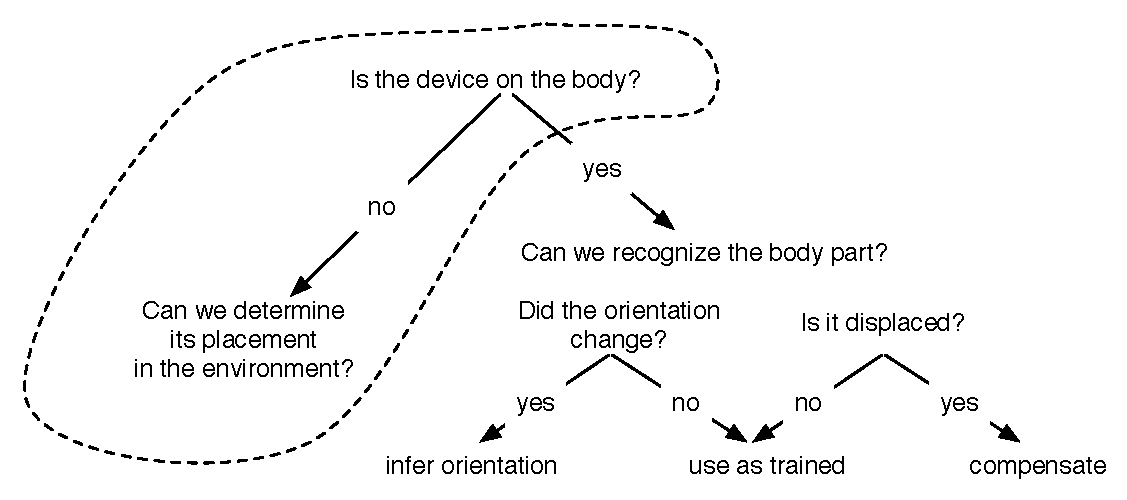
\includegraphics[height=2.4in]{OnOffOverview.pdf}
	\end{center}
\caption[Chapter content in relation to the thesis overview]{Thesis Overview marking the section dealt with in this
 chapter.} \label{fig:OnOffOverview} \end{figure} 
 To detect wether a device is carried on the body or placed in the environment is
 just a special case of recognizing the symbolic location of the
 device (see Figure~\ref{fig:OnOffOverview}). "Symbolic", in this instance, means assigning a label to a
 given device placement, e.g. "on the table", "in a draw". The
 symbolic location of an object can be interesting for a variety of
 reasons. Most obvious is the "where did I put my x" scenario. This
 scenario is highly relevant in so called assisted living
 systems. Such systems use on-body devices for behavioral monitoring
 and assistance for elderly and cognitively impaired persons. An
 important concern is to make sure that the user carries the device
 all the time. This implies checking if the device is on the user's body
 and, if not, using for example the TV, the radio or the phone to
 remind him to pick it up. In particular, for cognitively impaired
 users, it is important to be able to tell the user where the
 device is located, in case it was lost.

Trivially, whether the user carries a device on the body or not is
instrumental to using this device for context recognition. In fact,
knowing if the mobile phone is in a pocket, in the hand, or lying on a
table has been among the first suggested context sensitive
applications~\cite{schmidt1999aic}.
 Generally, we can use the location of smart objects as an indication 
 of user's needs. Thus, if a
device is put in the drawer where it is usually stored, it is
reasonable to assume that it will not be used in the near future and
it can go into power saving mode. Going even further the location of
a set of objects can be an indication of more general user activity
and intentions. Keeping in mind that placement on its own is a
valuable information source for context recognition systems, this
dissertation sees it more as being a low level part of an inference
chain, on which complex systems can be built.


The following assumptions are the basis for the remainder of this
chapter: \begin{enumerate}
\item Detecting wether a device is on the users body or not is a specific
 case of a more general problem inferring the symbolic location of an
 object.
\item Some context sensitive applications prefer symbolic
 classifications -- "on the shelf", "close to the printer" -- to absolute
 position coordinates.
\item The symbolic location classes introduced later are mainly chosen
 to show the merits and limitations of the given sensor modalities
 (acceleration and sound). They are, however, inspired by assisted
 living scenarios and can be used in such.
\end{enumerate}

To better understand how one can detect the symbolic placement, the
next section discusses different, proposed
solutions and related work followed by an exploration of environmental impacts on different sensing
modalities . Finally, we present our approach of active sampling the
environment with a rigorous experimental evaluation.


\section{Technical Possibilities and Related Work}

The simple straight forward way to deal with there environmental placement issues is
to integrate sensors directly into the symbolic location. Thus, there
is no need to recognize their placement as it is known and fixed after
manufacturing. Switches or accelerometers are placed on doors, the
stove etc. Prevalent intelligent home scenarios mostly apply this
option. Of course, this method entails all limitation of
infrastructure-based, fixed sensing.

Determining the symbolic placement of a device can be seen as a
specific case of indoor location estimation. Yet, indoor location is
known to be a hard problem. Hightower et. al. give a detailed overview about indoor localization techniques~\cite{hightower2001lsu}. 
As described above, our work aims at the localization of
simple objects in environments with no, or only minimal augmentation.
This means that many of the more reliable, standard methods are not
applicable. This includes ultrasonic location such as the BAT
 or the MIT cricket systems which
both require extensive instrumentation of the environment with
ultrasonic transceivers~\cite{128759,priyantha2000cls}. In addition ultrasonic system require free
line of sight and will fail to locate objects in closed
compartments. This means that infrastructure free, relative
positioning methods based on ultrasonics are
also unsuitable~\cite{1067190}. Cost and effort also make it infeasible using
complex time of flight based radio frequency (RF) methods such as the
commercial UBISENSE ultra wide band
system~\footnote{www.ubisense.net}. This holds, as well, for radio
frequency identification (RFID), requiring a reader or tag to be put
on every location which needs to be recognized.

\paragraph{Simple Beacon Based Systems}
Much work has been put into localization based on simple RF beacons,
often based on standard communication systems such as Bluetooth,
Zigbee and of course WLAN \cite{placeLab05,radar,krumm03ubicomp}. This includes a wide body of work on
positioning in wireless sensor networks \cite{dopigha01}. In
particular, work based on low power radio systems is clearly relevant
to object localization. This is more a complementary rather than a
competing approach. Such systems are virtually all based on signal
strength, which is inherently unreliable in complex, indoor
environments. As a consequence, they are predominantly used for room
level location (determining which room or large room segment a sensor
node is in). This is not sufficient for the type of symbolic location
targeted by this paper. However knowing approximate physical location
can be used to constrain the search space for our symbolic location
method.

\paragraph{Indirect Localization with Sensor Signatures}
Both sound and acceleration have been previously used in location related
research. Scott et. al. present a technique for performing accurate 3D location sensing using off-the-shelf audio hardware~\cite{scott05audiolocation} . 
Van Kleek et al. show some work in this direction, using sound fingerprints
to detect collocation~\cite{opf}.

The general concept of using acceleration signatures to extract
location related information can be traced to the 'Smart-Its Friends'
paper, \cite{smartits}. Building on this idea, Lester et. al. have
demonstrated how to determine if a set of devices is being carried by
the same person by correlating their acceleration
signatures~\cite{lester2004are}. In Chapter~\ref{chapter:onbody} we
take this concept even further, showing how acceleration signatures
can be used to determine where a user is carrying a device.

The most direct relation to the work presented in this chapter is a
patent by Griffin \cite{grifpatent} titled "User hand detection for
wireless devices". It proposes to use vibration detected by an
acceleration signal to determine if a mobile phone is in the user
hand, in a holster or in a holder.

\section{Environmental Placement Impacts}
It is reasonable to wonder what
impacts a specific placement has on a given sensing modality. We discuss these placement impacts on commonly
used pervasive sensing modalities, namely, motion, sound and radio
waves.

Motion sensors will receive no to little activation when they are
placed in the environment compared to being worn on the body. The
placement itself however can entail characteristic movements, e.g. the
vibrations of a fridge cooling aggregate.

\begin{figure}[t]
  \begin{center}
  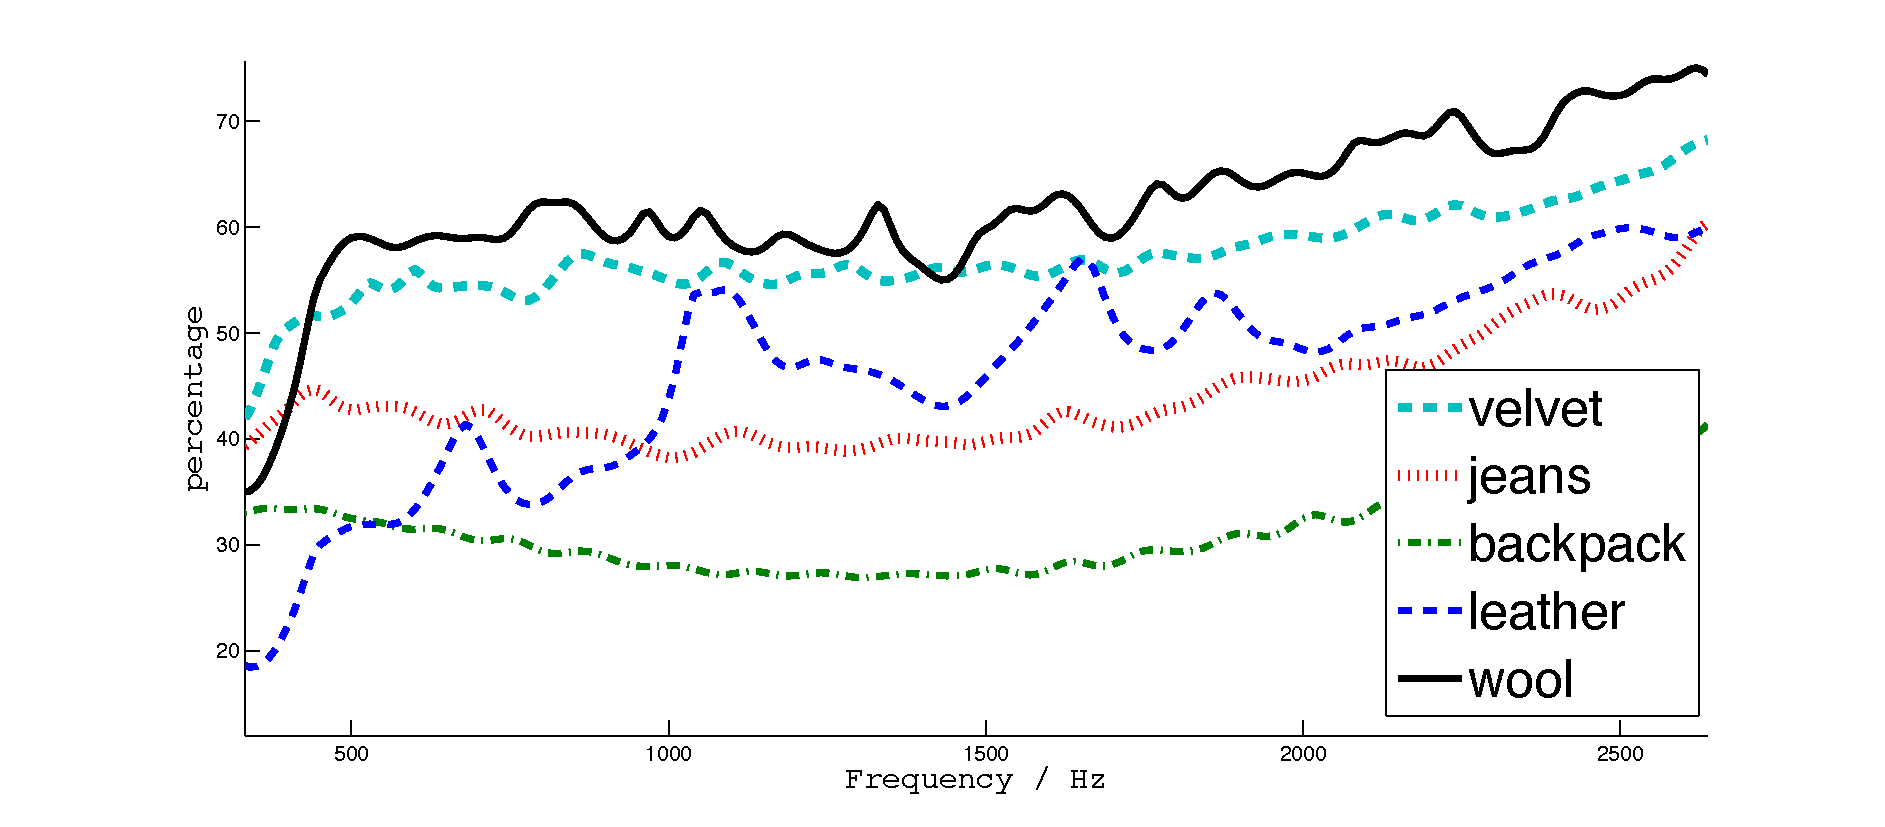
\includegraphics[height=2.5in]{soundplacement.pdf}
	\end{center}
\caption[Fabric dependent sound dampening]{Sound dampening depending on different fabric types. "White
 noise" in the frequency range from 500 to 2500 Hz is played on a
 regular pc speaker and recorded by an iphone 3gs. The iphone speaker
 is covered with the given fabric types. The plot shows the
 percentage difference between the clean recorded signal and the
 recordings obstructed by fabric. Each fabric has a distinct absorption spectrum.}
\label{fig:soundplacement}
\end{figure}

Changes in device placement affect sound to a much higher degree.
Different environments have their distinct sounds. As shown in
Figure~\ref{fig:soundplacement}, when the microphone of a device is
obstructed by specific material, frequency dampening is to be
expected. This is bad, if we try to classify sounds in the
environment. On the other hand, this dampening is distinct for the
given placement, therefore it can be used to determine the
location. This fact is explained in closer detail when we look at the
technical background of our method in section~\ref{onoff:background}.

\begin{figure}[t]
  \begin{center}
  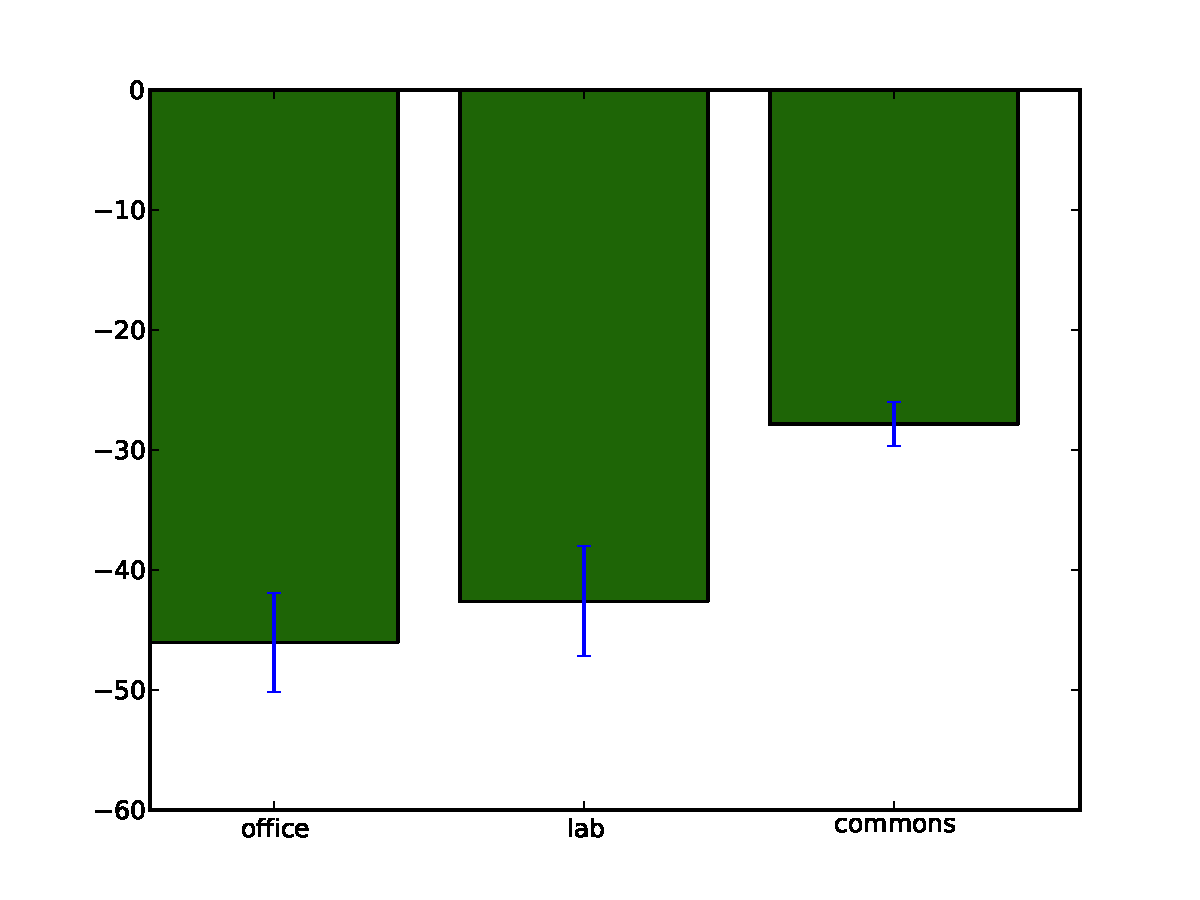
\includegraphics[height=2.5in]{sigstrengthRoom.pdf}
	\end{center}
\caption[Wifi signal strength for different rooms]{Wifi signal strength recorded by a mobile phone in
 different rooms of the same building. The phone is put on a desk
 for 5 minutes stationary in several rooms. The experiment is
 repeated 15 times. We show the mean average signal strength in dBm
  for three rooms: office, lab and commons. The difference in strength between rooms is statistically
 significant.}
\label{fig:sigstrength1}
\end{figure}

The environmental impact on radio waves is well known and
applied. There are several commercial efforts and an extensive
research body using these impacts, for example, for indoor location
technologies~\cite{hightower2001lsu, 1067190}. Radio waves, however,
are not only influenced by the environmental placement, but also by
their immediate surroundings; radio waves in the 2 GHz range, for
example, are obstructed by large amounts of water (e.g. the human body). As seen in
Figure~\ref{fig:sigstrength1}, the signal strength from several wifi
access points is distinct in different locations. However, the signal
strength also highly depends on the on-body placement of the device
recording it. 

As these examples illustrate, environmental placement affects sensor
signals in a complex way. There are specific locations that can be
distinguished using just passive sensor data, yet this method is very
limited regarding general placement inference. Thus, the approach to
actively sample the environment (i.e. the device itself emits a given stimulus and analyses the
response of the environment) seems to be far more promising.


\section{Theoretical Background}
\label{onoff:background}
Our method is derived from the observation that a ringing mobile phone
sounds differently depending on where it is located. Whereas a phone
in a jacket pocket sounds 'dampened', a phone on a metal cabinet can
make the entire cabinet resonate. This is true for a ringing phone as
well as for a merely vibrating phone. We, thus, propose to use sound from
a built-in speaker and vibration from a built-in vibro-motor to create
a mechanical "excitation" of the environment and analyze the response
with an accelerometer and a microphone.

%a microphone. In an extensive experimental 
%study (47 locations with total of 1200 data points) 
%we demonstrate that two types of information can be derived from this analysis. 
%First, the system can be trained to recognize
%specific locations such as the 'kitchen table', or the 'dining room
%table'. Second, it can recognize more abstract locations based on
%materials such as a 'wood table', 'a closed metal cabinet', or a 
%'jacket pocket'. While this leads to less specific positioning, it has
%the advantage that the system does not need to be trained for each
%single location. Instead, after being trained on, for example, 
%several wood tables, it will recognize others it has not seen before.

%Clearly understanding how object location can be used in different
%applications is a complex topic that needs further research. 
%Nonetheless, the type of considerations sketched
%above indicates that object location is 
%a useful piece of information.
%% and finding ways to obtain it with 
%%simple, easily deployable setup a relevant research topic. 
%From this motivation we
%present and systematically evaluate a novel method for 
%object localization. The method provides so called symbolic (sometimes
%also called semantic) location (e.g. \cite{1045120})
%rather then absolute coordinates. Thus the output of the system is of
%the type 'on the couch' or 'in the drawer'. 
%The key contribution of our work is to present a
%method that requires no infrastructure, relies on simple, cheap
%sensors and still produces useful results.

In abstract terms, the above method is about analyzing the response
of the environment to a mechanical "excitation" with different frequencies. 
By vibrating the device we provide a low frequency (a few Hz) and relatively high intensity (as
compared to sound) source of excitation. By emitting fixed frequency
"beeps" we generate different, low intensity high frequency stimuli.  
The accelerometer detects the low frequency response (in our case up
to 15Hz due to a device sampling frequency limit of 30Hz),
the microphone the high frequency part. 

The response to the above stimuli falls into several categories. 
First, we receive a low frequency response. 
It is directly mechanically coupled to the vibrating object and can be detected
by the accelerometer. This response can range from a more or less
complete absorption of the vibration energy (e.g. when the object is
lying on pillow) to a resonant response where the 
surface on which the device is lying, joins in the vibration.
This fact contains information on two placement properties. For one, it can reveal if, and how
the device is fixed (in the hand, in a tight pocket, lying freely). In
addition, it reveals the hardness and elasticity of the surface on which the
device is placed. This information can be expected to reliably distinguish
between soft surfaces (e.g. a sofa) and hard ones like a
table. Distinction between several similarly hard surfaces (e.g. metal
and stone) is difficult.

Second, we get a high frequency response from the vibration, 
which is essentially sound from the device hitting the
surface. Assuming the placement of the device does lead to this kind
of response (it will not, if the device is in a soft pocket or say hanging),
it is quite location specific. The sound depends not only on the
surface material but also on the overall structure. 
Thus a small, solid cube will produce a different sound
than a large thin surface, even if both are made of the same
material. Finally, objects light and close enough to the device to
be influenced by the vibration (e.g. a key chain) might also
contribute to the sound. In general, this is a source of noise rather
then usable information. 


 Third, we get a high frequency response from the beeps which
is given by the absorption spectrum of the environment.~\footnote{Note that the absorption also influences the sound caused by the device vibration.}
Clearly this response is only useful if it comes from the immediate
vicinity of the device. This can either be the surface on which the
device is lying or, if the symbolic location is a closed compartment, the
walls of this compartment (see sections 2.4 and 2.7 for a discussion of
microphone placement issues). 

\begin{table}[ht]
\caption[Frequencies and material absorption spectrum]{Frequencies and their absorption by the selected material, given as a fraction of perfect absorption\cite{olson1967mpa}.}
\centering
\scalebox{0.95}{
\begin{tabularx}{40pt+\textwidth}{l c c c c c c }
\toprule
frequency & 128 Hz &	256 Hz &	512 Hz &	1,024 Hz &
2,048 Hz & 	4,096 Hz \\
\midrule
concrete unpainted & 0.010&	0.012&	0.016&	0.019&	0.023&0.035 \\
brick wall painted & 0.012&	0.013&	0.017&	0.020&	0.023&0.025 \\
carpet on concrete & 0.09 &	0.08 &	0.21 &	0.26 &	0.27 &0.37 \\
\bottomrule 
\end{tabularx}}
\label{table:freq} 
\end{table}
 
It is well known that the acoustic absorption spectrum is a distinct
material property. The topic has been extensively studied in the
context of musical instruments and sound isolation in
construction~\cite{olson1967mpa}. Typically, the absorption is given at discrete
frequencies as a fraction of the perfect absorption of an open window
(lack of any reflecting surface) of equal area.
As an example, we consider the coefficients in Table~\ref{table:freq}.
This clearly demonstrates that, in principle, even seemingly similar materials
can be separated with a small number of discrete frequencies. 

\section{Approach}
\label{sec:approach}
\paragraph{Procedure Description}
The proposed method consists of two parts. Each part can be used
individually or in combination with the other.

The first part is based on vibrating the device using a 
vibration-motor of the type commonly found in mobile phones. During
the vibration, which last a couple of seconds, motion data is recorded with
an accelerometer and sound with a microphone. The motion and sound
signals are used separately for an initial location
classification using standard feature extraction and pattern 
recognition methods. The final classification is obtained
through fusion of the two classification results. 

The second part is based on sound sampling. The device emits a series
of beeps, each in a different, narrow frequency spectrum. The
microphone is usually positioned is such a way that it receives only little energy
directly from the speaker. Instead a significant part of the energy
comes from reflections from the immediate environment (see bellow 
for a more detailed discussion). For location
recognition the sound received from the different beeps is compared. 

When the two parts are used together, the corresponding results are
fused using an classifier fusion method. 

\paragraph{Applying the Procedure: Specific Locations vs. Location Classes}
 Our method provides information on
abstract properties such as surface material as well as information
on properties characteristic of a single specific location (e.g. a
solid cube vs. large surface with several legs). As a consequence this
chapter investigates two different usage modes of our method:
\begin{enumerate}
\item "Specific Location Mode". In this mode, we train the system on
 concrete locations such as a specific table or a specific chair. The advantage of this approach is that the user
 is provided with exact location information. The main disadvantage is the
 effort involved in training each individual location. In addition,
 there is the question of being able to distinguish a large enough number of
 locations to satisfy relevant applications. 
\item "Abstract Location Class". In this mode, we group locations into
 abstract classes. The two main criteria are the surface material and
 being open (e.g. tabletop) or closed (e.g. inside a cupboard). In
 this mode the system is trained on several instances of each
 class. It is then able to recognize other arbitrary instances of
 this class. Thus the training problem is avoided, as the system can
 pre-trained at 'production time' and given to users without the need
 for further training. The disadvantage lies in the less exact
 location information, which has to be further interpreted and/or
 combined with additional information to find out where the object is
 actually located.
\end{enumerate} 

\subsection{Issues to Consider}
\label{sec:issues}
\paragraph{Microphone and Speaker Placement}
As described above, for the analysis of the absorption spectrum we must
ensure that the sound emitted by the loudspeaker is reflected from the
surface on which the device is lying and/or, in case of the symbolic
location being a closed compartment, from the compartment walls. The
second part is trivial. The first implies an appropriate placement of
the microphone and the speaker. 
Optimally the speaker and the
microphone should be located close to each other
on the side of the device, preferably (but not necessarily) 
facing downwards with a sound proof
barrier blocking the direct sound path between them. The main problem
in implementing this type of setup is the definition of "on the side"
and "downwards". In the worst case, we could be dealing with a cubic
or round object with no preferred "down" or "side". For such an object,
two speakers located at a 90 degree angle 
need to be used to ensure that there is always a sidewards
facing one. Our experiments (see section \ref{sec:experimental})
indicate that the position of the microphone is less critical and we
achieved good results despite the microphone facing upwards, so that
one microphone might suffice. 

%It is interesting to note, that the results of our experiments indicate
%that optimal placement is not critical. The NOKIA mobile phone
%used in the experiments indeed has a loudspeaker on the side (upper
%side see figure \ref{fig:nokia}) facing towards the back side. If
%placed in the usual position (back side down) this means that the
%loudspeaker is facing downwards towards the surface. 
%However the microphone is on the
%front side (which is then the upper side) on the lower end of the
%phone. This is a quite typical layout for modern mobile phones which
%ensures that the 'hands-free' speaker will not be accidentally put to
%the ear when on.
 
\paragraph{Variations within Symbolic Locations}
Many symbolic locations such as "table" or "desk" 
have considerable physical dimensions. This means that the response to
the mechanical stimuli may be subject to spatial
variations. For example, the low frequency 
response to vibration (acceleration data) may be different over the
leg of a table than in its middle. Similarly, on a table adjacent to the
wall, the response to the "beep" will vary depending on how close to
the wall the device has been placed.
As a consequence, for both, training and testing, a sufficient number
of random physical locations must be sampled for each symbolic
location (as has been done in experiments described in section \ref{sec:experimental}).

\paragraph{Number of Relevant Locations}
Clearly there are limits to how many locations can be reliably
recognized. In common environments
such as home or office, there are many 
places where objects can be put. The question is, whether the
number of locations that can be distinguished is sufficient to be
useful in relevant applications. An authoritative answer to this
question can only be found through an analysis of specific 
applications. Subsequently, we make no claim for such an answer,
we focus on the technology merits instead, demonstrating the
following:
\begin{enumerate} 
\item Our system shows reasonable recognition performance even using
 the combined data set of 35 locations. In our experiments these are
 collected from 3 rooms. It seems unlikely that this would not
 be sufficient covering all relevant symbolic locations in a 
 single room. At the same time, room level location of RF enabled sensor nodes is a manageable problem. 
\item Provided that an adequate number of sufficiently abstract
 classes is chosen, the issue of the number of locations is avoided by the
 "abstract location classes" usage mode. In the experiments, we
 demonstrate near perfect recognition for 7 and reasonable results
 for 12 classes. The type of classes used in the experiments ("open
 wood surface", "closed wood cabinet" etc.) is clearly abstract
 enough to describe a large number of locations. 
\end{enumerate} 

\paragraph{Sensor Requirements}
In the introduction we have stated our aim of developing a method
suitable for smart objects. Accelerometers and a microphones are
among the most widely used components in small sensor nodes. Small
loudspeakers capable of emitting beeps are also commonly integrated in those
nodes. As will be described in section \ref{sec:recognition} 
we work with frequencies between 500 and 4000 Hz, which can be handled
by small, cheap speakers and microphones. Finally, although 
vibration motors have so far not been used in sensor nodes, they are
available in sizes around 1cm and smaller (see figure \ref{fig:vibmot})
at reasonable costs. 

In summary it can be said that the proposed sensor configuration is 
compatible with the target domain of small, cheap smart objects. 

\paragraph{Complexity}
Any method that is to be deployed on low end sensor nodes and smart
objects needs to be resource conscious.
However, when considering the method proposed in this paper it is important to
remember that it is not meant for continuous tracking of a
moving device. Instead we assume that the method runs once
after the acceleration sensor has detected that the device has been
moved and is left to rest. Therefore, speed and power efficiency of the algorithm
are not so essential. We just need to
show that with typical resources available in such nodes
it is feasible to either perform the required computation or transmit
the data to a remote server for processing.
For the sake of simplicity, we restrict ourselves to the
communication requirements of the raw data.
With 16 bit resolution and the sampling rates
given in section \ref{sec:recognition} we require a data rate of about
130 Kbps for the sound and a about 5 Kbps for the acceleration. These rates
have to be sustained for a total of 13 seconds.

With respect to online execution, we merely point to related work by
our group in which we have studied implementations of sound and
acceleration based activity recognition\cite{1033880}. With sampling rates, features
and classifiers similar to the ones proposed in this paper we were able
to demonstrate power efficient execution on nodes using the TI MSP 430
microcontroller with less then 100K of RAM. 
Therefore, a sensor node should be able to execute the proposed method
--or at least computing most of the features (in particular the FFT)--
to avoid transmitting the raw sound data.

%\subsection{Usage Modes and Limitations}
%As stated in the introduction 
\section{Recognition Method}
\label{sec:recognition}
As described in section~\ref{sec:approach}, our approach can be divided into two distinct methods, mechanical vibration and sound sampling. 

\begin{table}[ht]
\caption{Features used for frame-by-frame classifications}
\begin{center}
\begin{tabularx}{\textwidth}{XX}
%{p{1.95in}p{2.95in}}
\toprule
Feature Name& Description\\
\midrule 
Standard features& Zero Crossing Rate, median, variance, 75\% percentile, inter quartile range\\
\midrule 
Frequency Range Power& computes the power of the discrete FFT components for a given frequency band. \\
\midrule 
Sums Power Wavelet Determinant Coefficient 
& describes the power of the detail signals at given levels that are derived from the discrete wavelet transformation of the windowed time-domain signal. This feature has successfully been used by \cite{sekine2000}. \\
\midrule 
Root Mean Square (RMS)&$\sqrt{\frac{1}{N}*\sum_i{x_i^2}}$, with $N$
the number of samples in a sliding window, and $x_i$ the i'th sample of the window.\\
\midrule 
Number of Peaks& The number of peaks in the window with different thresholds, low medium and high.\\
\midrule 
Median Peak Hight& The median of the peak hight. \\
\bottomrule
\end{tabularx}
 \label{table:features}
\end{center}
\end{table}

\subsection{Vibration}
During the vibration phase, the device itself records the sound and the
acceleration. Figure~\ref{fig:soundVib} and Figure~\ref{fig:accelVib} show some signal examples for
sound and acceleration recorded in different symbolic locations. Classification is performed separately on
each signal and the information of the two
modalities is combined on classifier level (see Section~\ref{sec:fusion}).


\begin{figure}[t]
  \begin{center}
  \subfloat[]{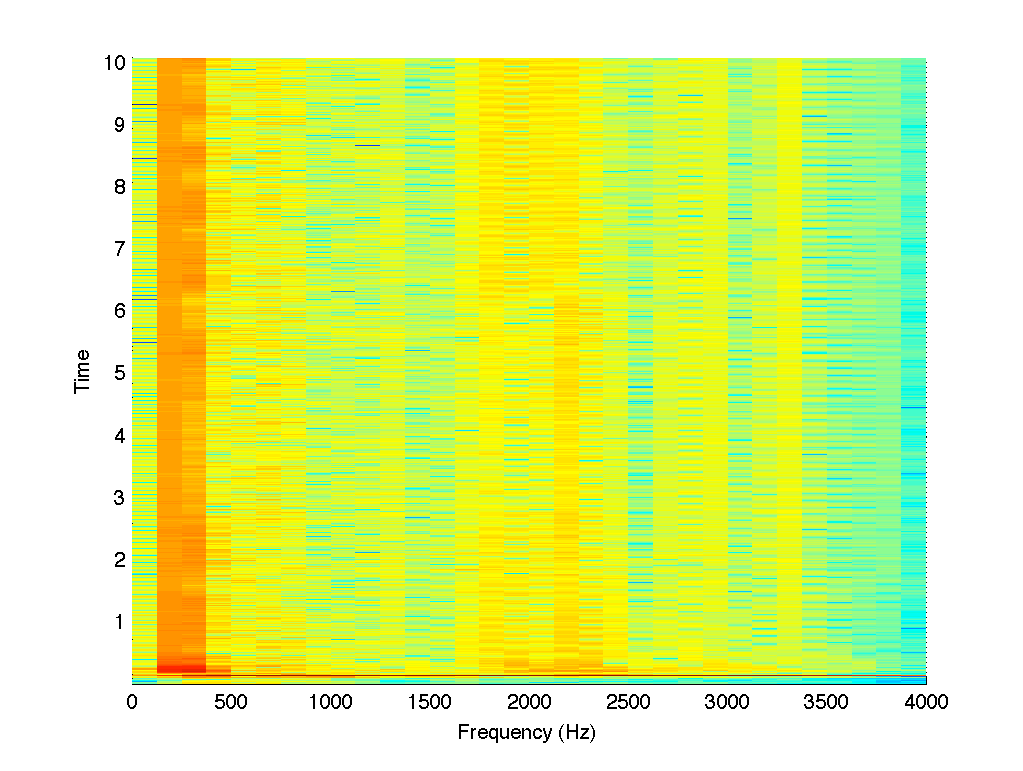
\includegraphics[trim=10 0 10 0,clip,height=1.7in]{carpetfloor-vib.pdf}
  	\label{fig:carpetVib}}
  \subfloat[]{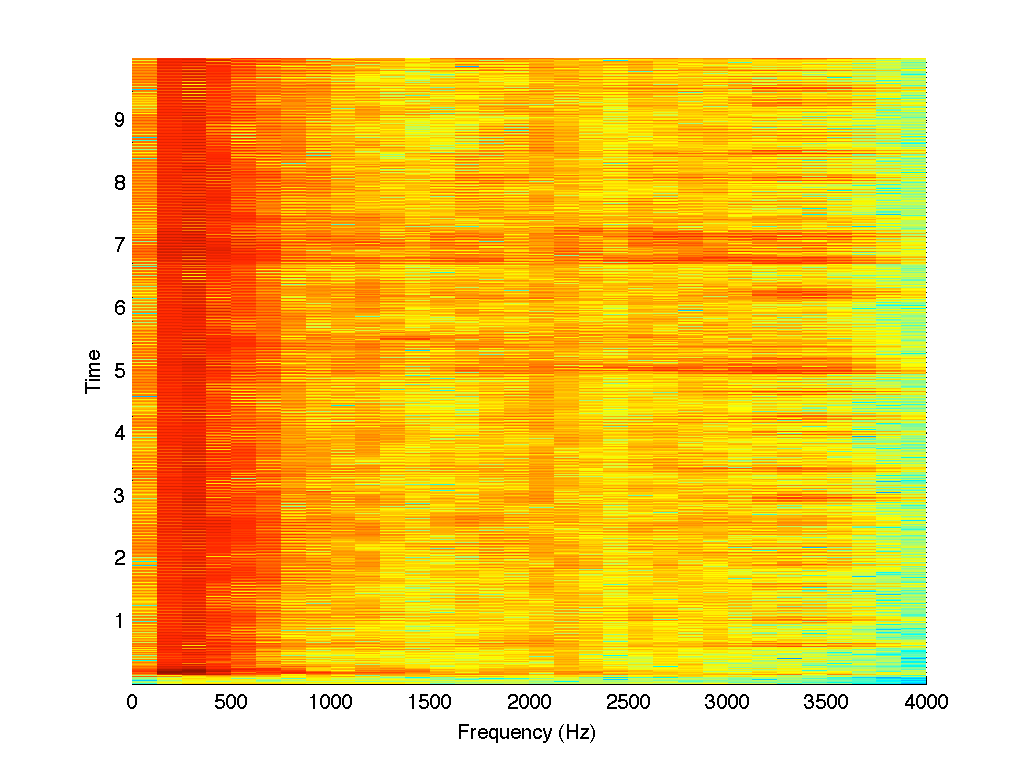
\includegraphics[height=1.35in,height=1.7in]{desk-vib.pdf}
  	\label{fig:deskVib}}
   \end{center}
\vspace{-10pt}
\caption[Sample vibration sound spectrum]{
The vibration sound spectrum recorded for a carpet, on the left, and a desk, on the right.}
\label{fig:soundVib}
\vspace{-10pt}
\end{figure} 

\paragraph{Vibration Sound Processing}
About 30 individual features are calculated
over a 500 msec. sliding window (250 msec. overlap). We
pick 5 based on initial tests: the zero
crossing rate, the frequency range power, 75\%Percentile, sums power
wavelet determinant coefficient and the median (see Table~\ref{table:features}). We
trained common machine learning algorithms using these features, e.g. K-NN, Naive Bayes, C
4.5. As all machine learning algorithms provid comparable results and we need a ranking mechanism for the different
classes, we use the Naive Bayes classifier in the following. 
The frame-by-frame output provided by the Naive Bayes classifier is
smoothed using a majority decision over the entire length of a single
vibration phase. We also perform experiments using Hidden
Markov Models either on the features calculated in the 500ms windows
or on the classifier output of the frame by frame classifier. Since
none of the above produced significant improvement, we use
the less computationally intensive majority decision.


\begin{figure}[t]
  \begin{center}
  \subfloat[]{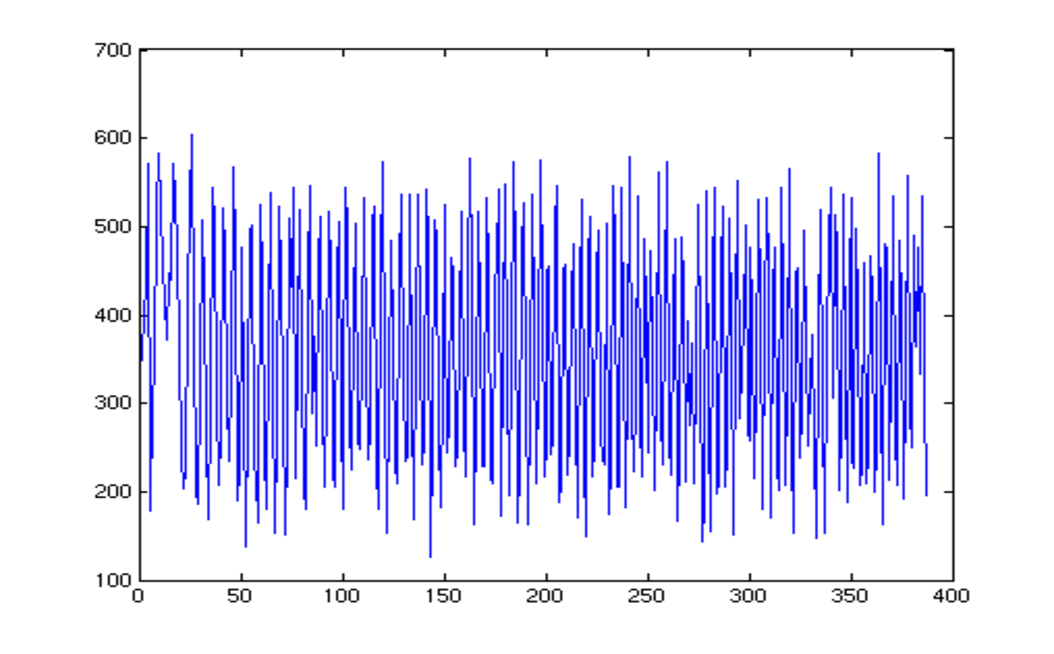
\includegraphics[height=1.7in]{bed.pdf}
  	\label{fig:bed}}
  \subfloat[]{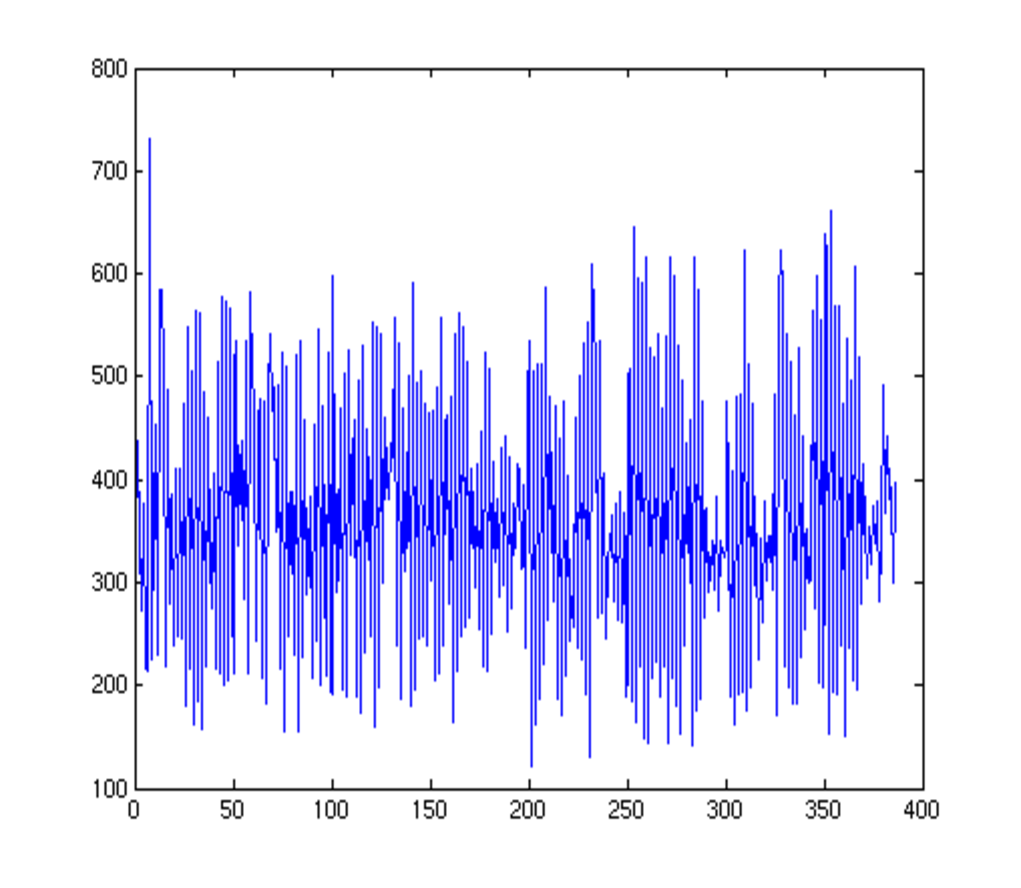
\includegraphics[height=1.7in]{stereo.pdf}
  	\label{fig:stereo}}
   \end{center}
\vspace{-10pt}
\caption[Acceleration norm examples]{
The acceleration norm from 
bed~\subref{fig:bed} and the stereo~\subref{fig:stereo}. On the x-axis are the samples (30 per second) and on the y-axis the magnitude. The accelerometer on the Nokia 5500 Sport discretizes the values between +/- 600, 250 being 1 g.}
\label{fig:accelVib}
\vspace{-10pt}
\end{figure} 


\paragraph{Vibration Acceleration}
The process described above for the vibration sound is essentially
repeated for the acceleration. The only differences are the length of
the window  (1 sec with 0.5 sec. overlapping) and the final feature
set (variance, the RMS, number of peaks, median peak height, the
75\%Percentile, inter quartile range). 

\subsection{Sound Sampling}

\begin{figure}[t]
\centering  
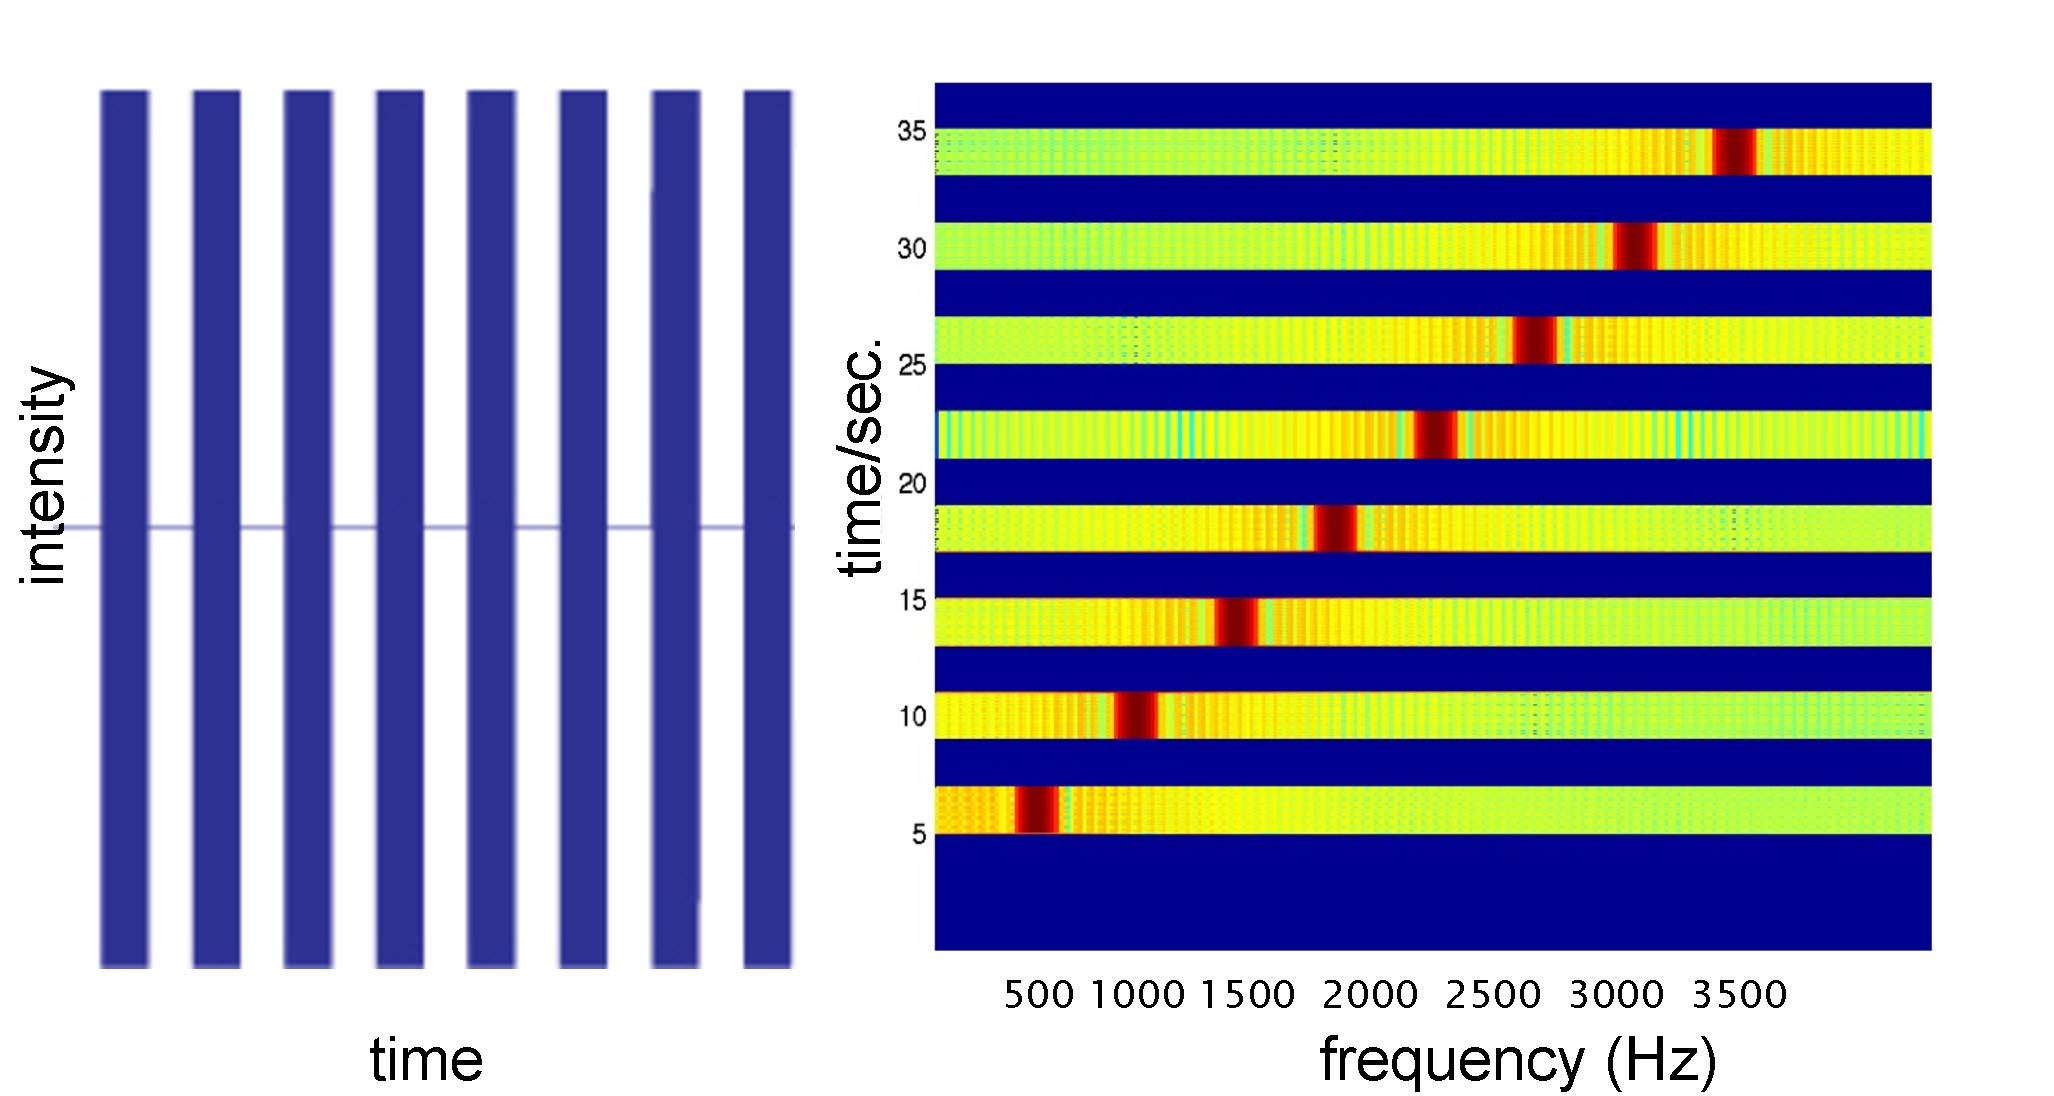
\includegraphics[scale=0.36]{beeps.pdf}
\caption[Audio fingerprint sample]{The played fingerprint audio, with the distinct frequencies, on the left in the time domain, on 
the right in the frequency domain.}
\label{fig:beeps}
\end{figure}

\begin{figure}[t]
  \begin{center}
  \subfloat[]{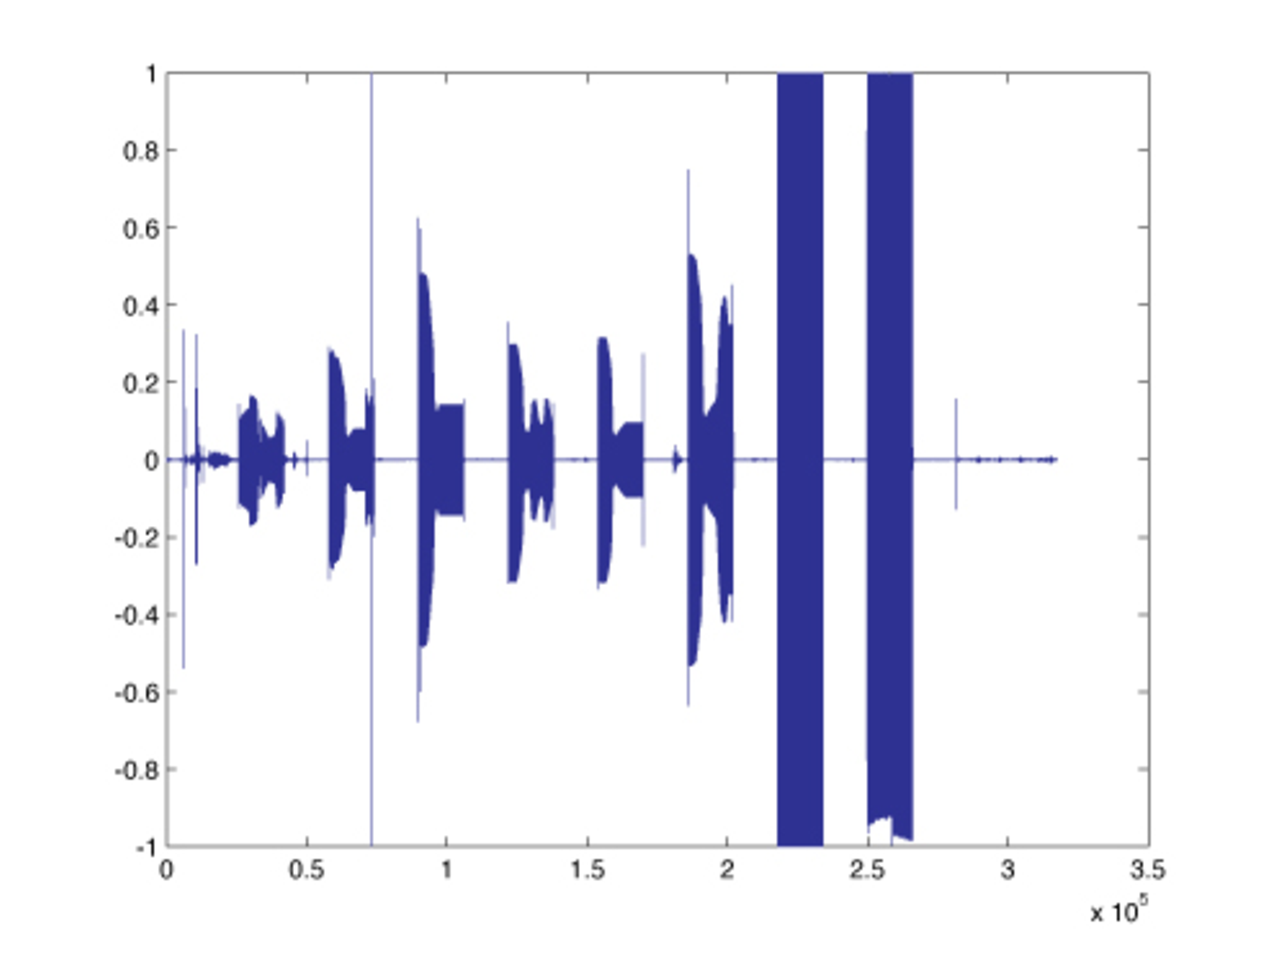
\includegraphics[height=1.7in]{drawer.pdf}
  	\label{fig:drawer}}
  \subfloat[]{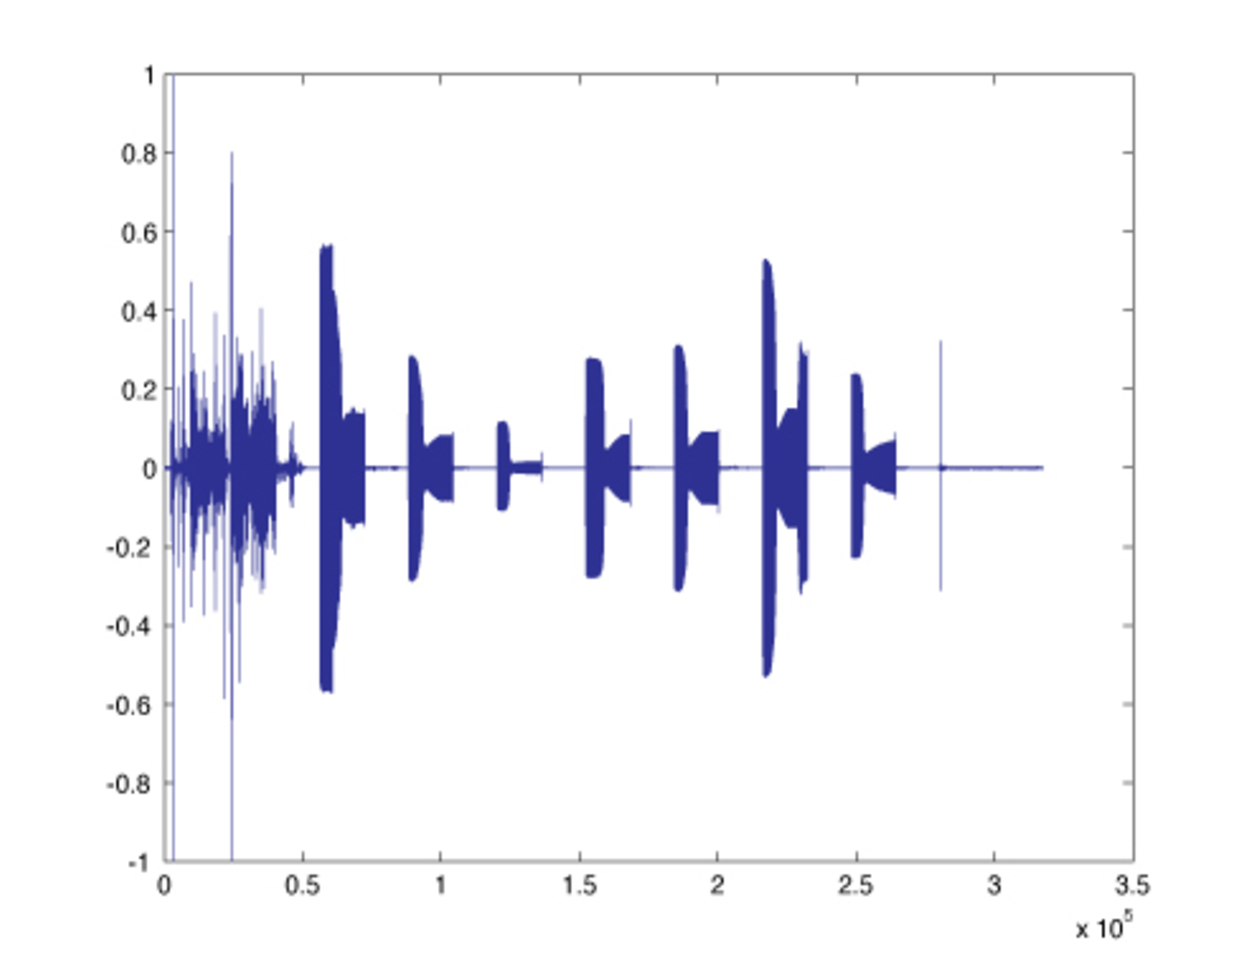
\includegraphics[height=1.7in]{backpack.pdf}
  	\label{fig:back}}
   \end{center}
\vspace{-10pt}
\caption[Time domain audio fingerprint examples]{
The audio fingerprints for drawer and backpack in the time domain}
\label{fig:soundfing}
\vspace{-10pt}
\end{figure} 


\begin{figure}[t]
  \begin{center}
  \subfloat[]{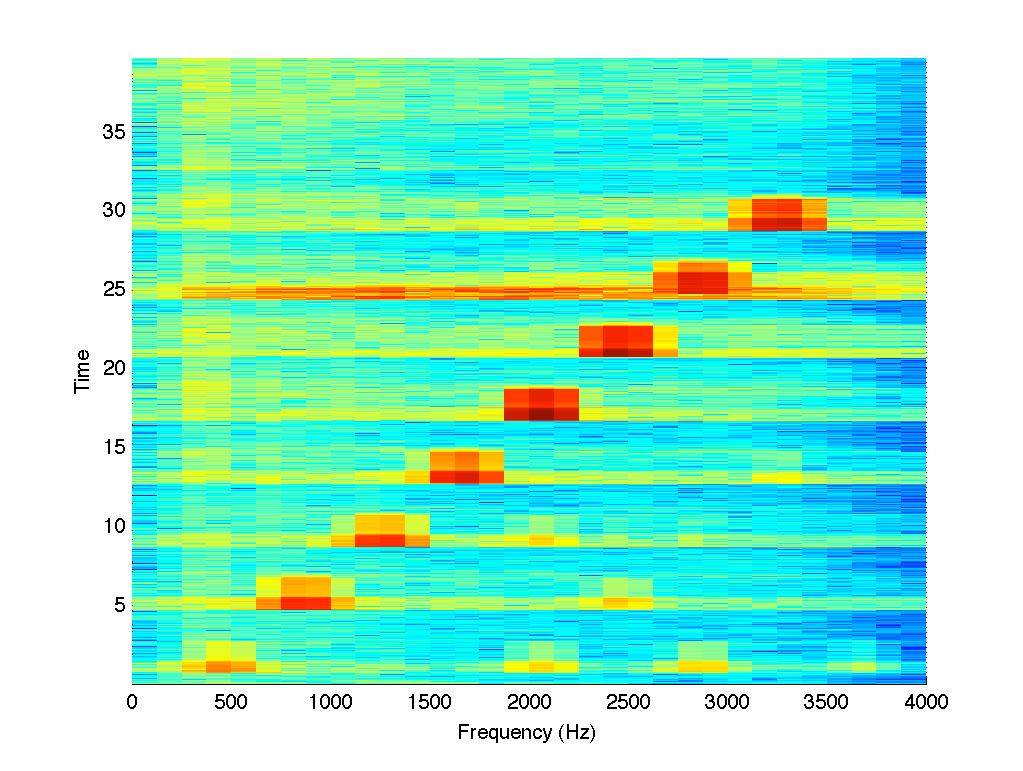
\includegraphics[height=1.7in]{shelffingerprint.pdf}
  	\label{fig:backf}}
  \subfloat[]{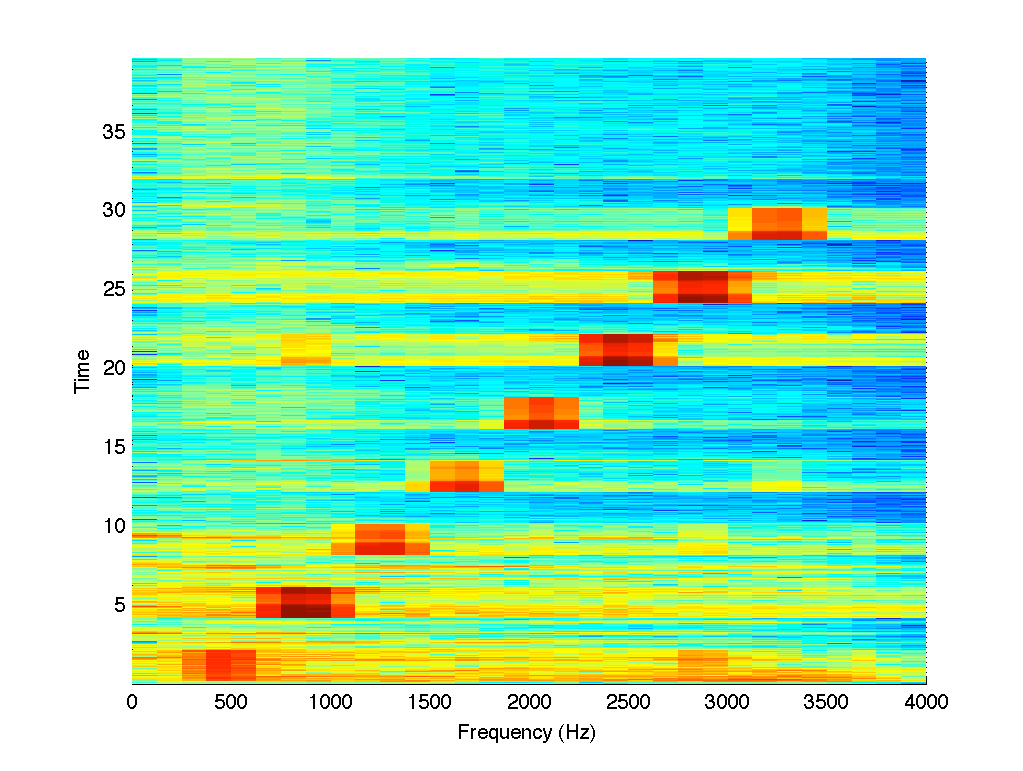
\includegraphics[height=1.7in]{backpackfingerprint.pdf}
  	\label{fig:drawerf}}
     \end{center}
\vspace{-10pt}
\caption[Frequency domain audio fingerprint examples]{
The audio fingerprints for drawer and backpack in the frequency domain}
\label{fig:soundfingt}
\vspace{-10pt}
\end{figure} 

The active sound sampling procedure differs from 
the vibration method in several 
ways. We know from literature (see section \ref{sec:approach}) that
few discrete frequencies between a few hundred and a few thousand Hz are enough to separate a large range of
materials in terms of their absorption coefficients. Therefore, we 
select 8 discrete, equidistant frequencies 
between 500 and 4000. Figure~\ref{fig:beeps} shows the signal emitted by the speaker in time and frequency domains. 
The frequency range choice is dictated
by the specification of small, cheap speakers (not capable of very low
frequency tones) and available sampling rates -the used mobile phone is just capable of sampling
with 8000 Hz. Some sample recordings for different symbolic placements can be seen in
Figure~\ref{fig:soundfing} (in the time domain) and in Figure~\ref{fig:soundfingt} (in the frequency domain). 
From the recorded beeps we first isolate 8 frequency fingerprints
using a variable intensity threshold. As features we empirically select
RMS, frequency range power and the sums power wavelet determinant
coefficient using the mutual information metric. These features 
are determined out of 30 features calculated using a 200
msec. sliding window with 150 msec. overlap.

The features of all 8 frequency prints are combined into one feature set.
This means that a feature instance contains the calculated RMS etc. of each 
frequency band. The rest of the procedure is identical with the 
vibration recognition (frame by frame classification using C 4.5 and
majority decision). 

%Machine learning algorithms are trained on the feature set, here again we picke
%d the C.4.5 as final classifier. On top of the frame-by-frame classification a 
%majority
%voting is employed for the complete duration of the recorded sound sample.

\subsection{Fusion}
\label{sec:fusion}

\begin{figure}[t]
\centering  
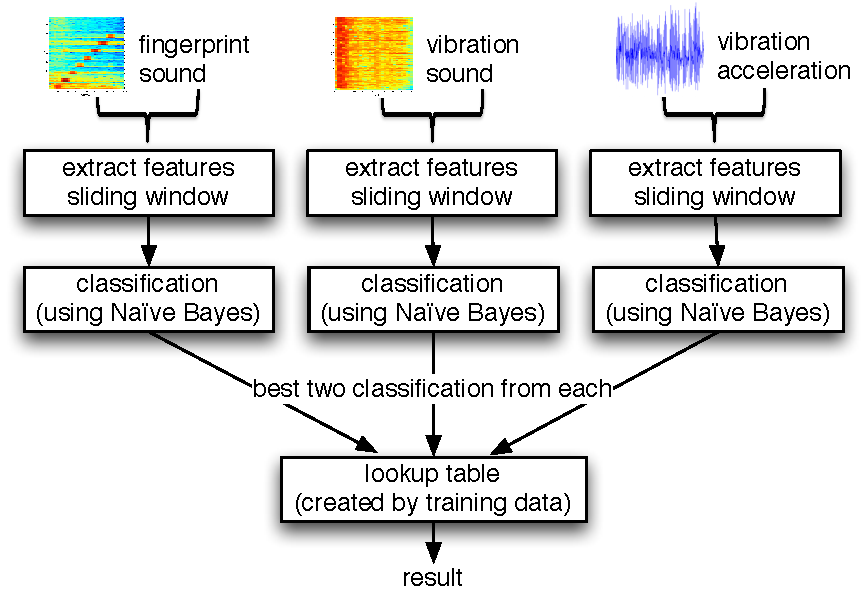
\includegraphics[scale=0.66]{recognition2.pdf}
\caption{The fusion recognition method as overview.}
\label{fig:recognition}
\end{figure}
The two main approaches to fusion are signal/feature level and
classifier level fusion. Feature level fusion works best for features
that are computed at the same sampling rate (sliding window size).
This is not the case for the three recognition modalities described
above. As the different window sizes are determined heuristically to
produce best results for each modality, dropping them for the sake of
fusion makes little sense. As a consequence, no direct feature level
fusion is investigated. We, however, investigate a fusion
approach based on the results of the 
frame by frame classification (see Figure~\ref{fig:recognition}). This can be viewed as a kind 
of feature level fusion, since its result is
input to the majority decision. Thus, we compute
the majority decision for an event over the frame by frame results
from all three modalities put together, instead of computing it for
each modality separately.

In terms of classifier fusion we opt for a Bayesian Belief
Integration method (see \cite{ruta-overview} for an overview of
classifier fusion methods). This method uses the confusion matrix
obtained from testing the classifiers on the training data set to
determine class probabilities for different combinations of
classifier outputs. This allows the system to take into
account the peculiarities of each classifier. 
With just 3 classifiers and a constrained number of classes 
it is also computationally tractable. If the number of classes 
is increased the method could be replaced by e.g. logistic regression.

\begin{figure}[t]
  \begin{center}
  \subfloat[]{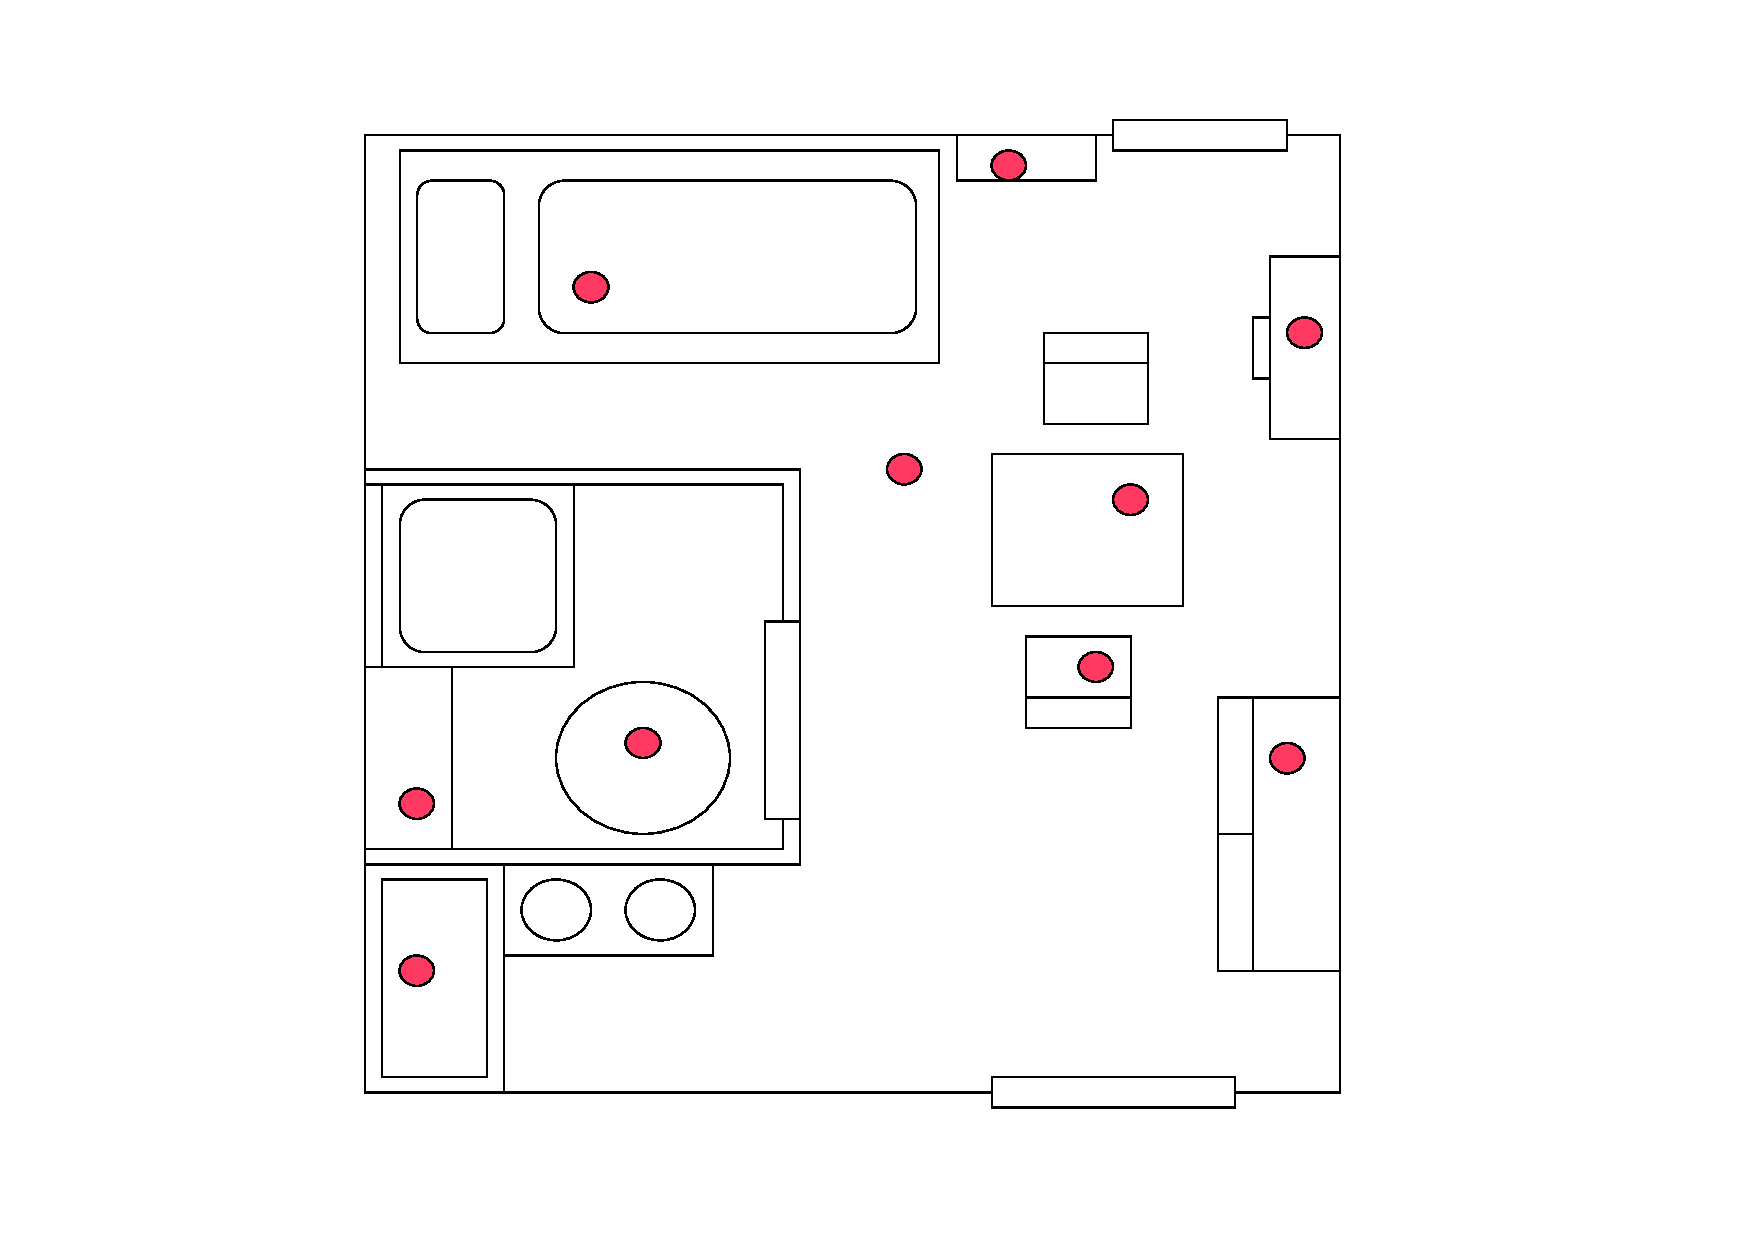
\includegraphics[trim=10 0 10 0,clip,height=1.7in]{appartment.pdf}
  	}
  \subfloat[]{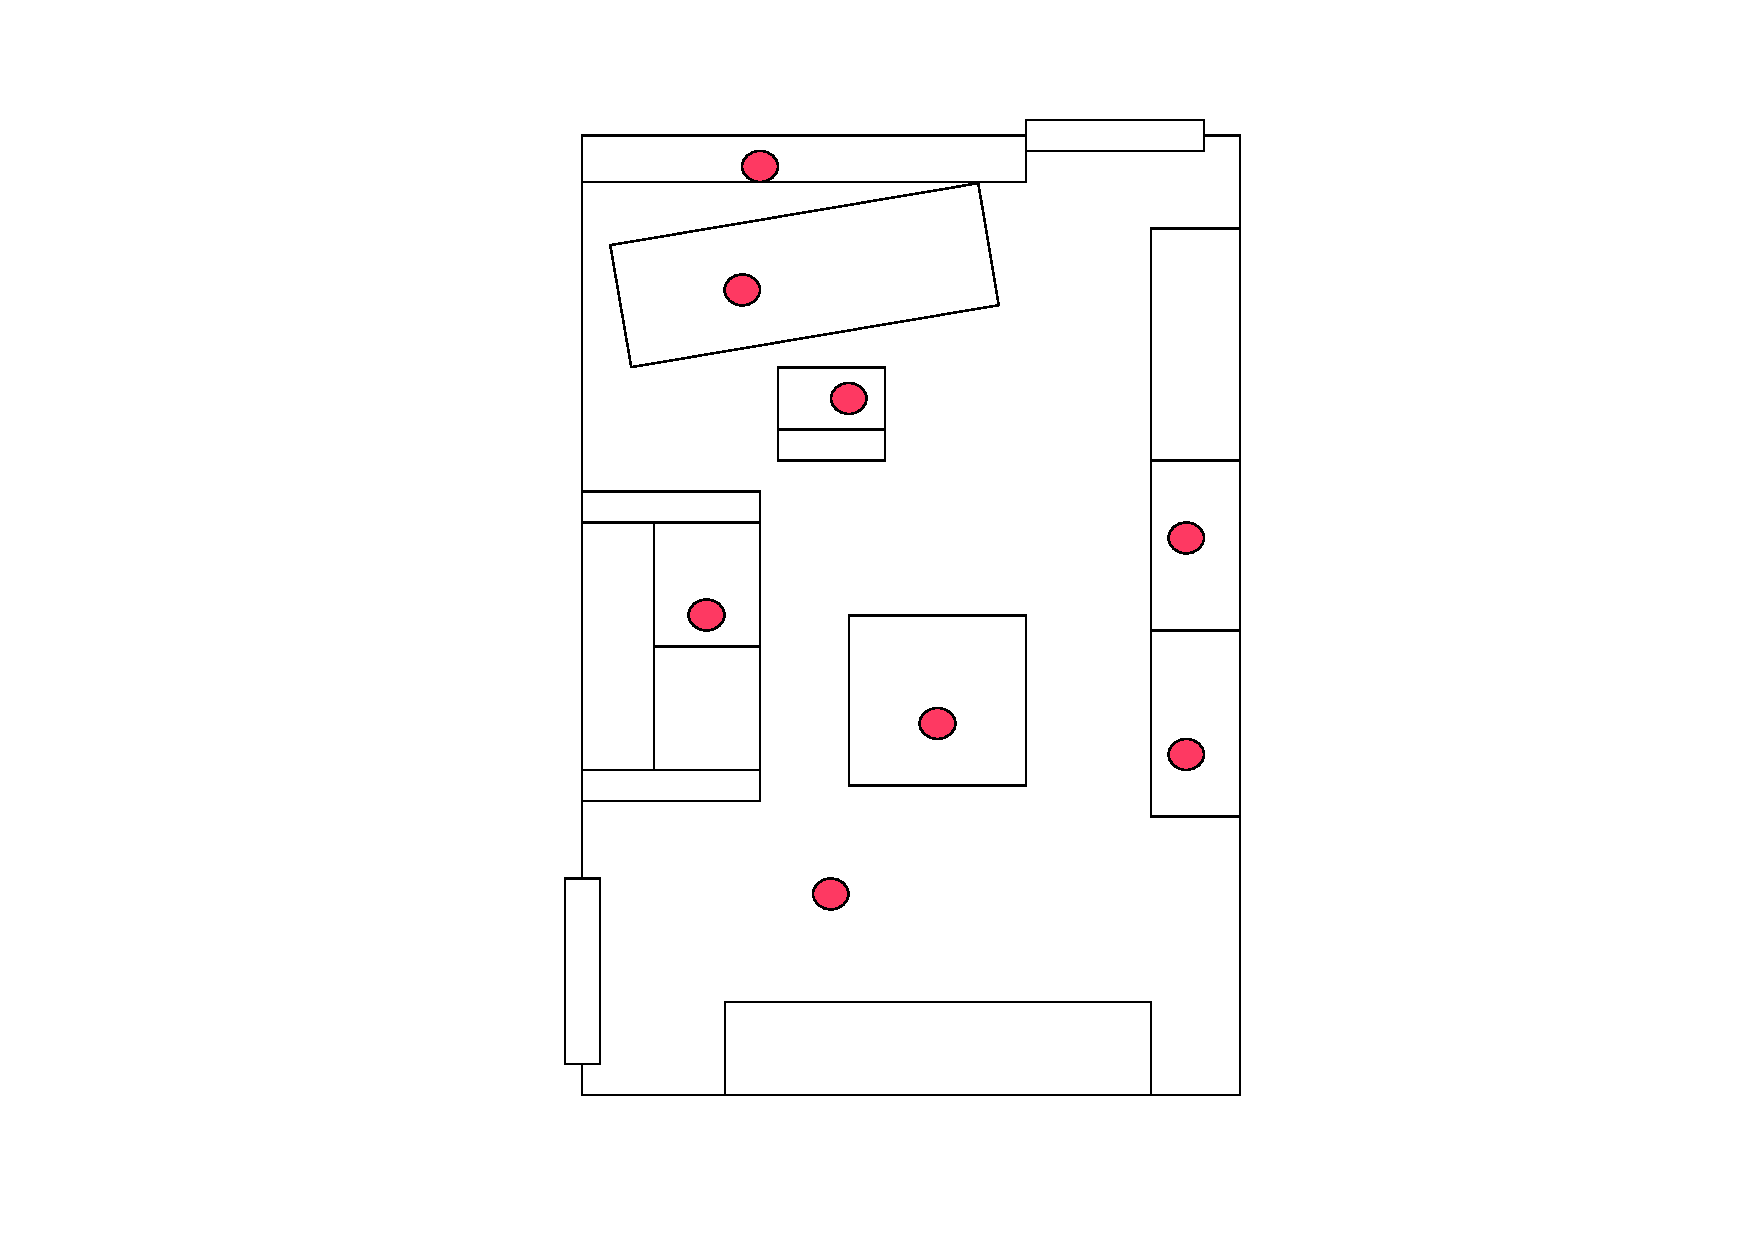
\includegraphics[height=1.35in,height=1.7in]{livingroom.pdf}
  	}
 \subfloat[]{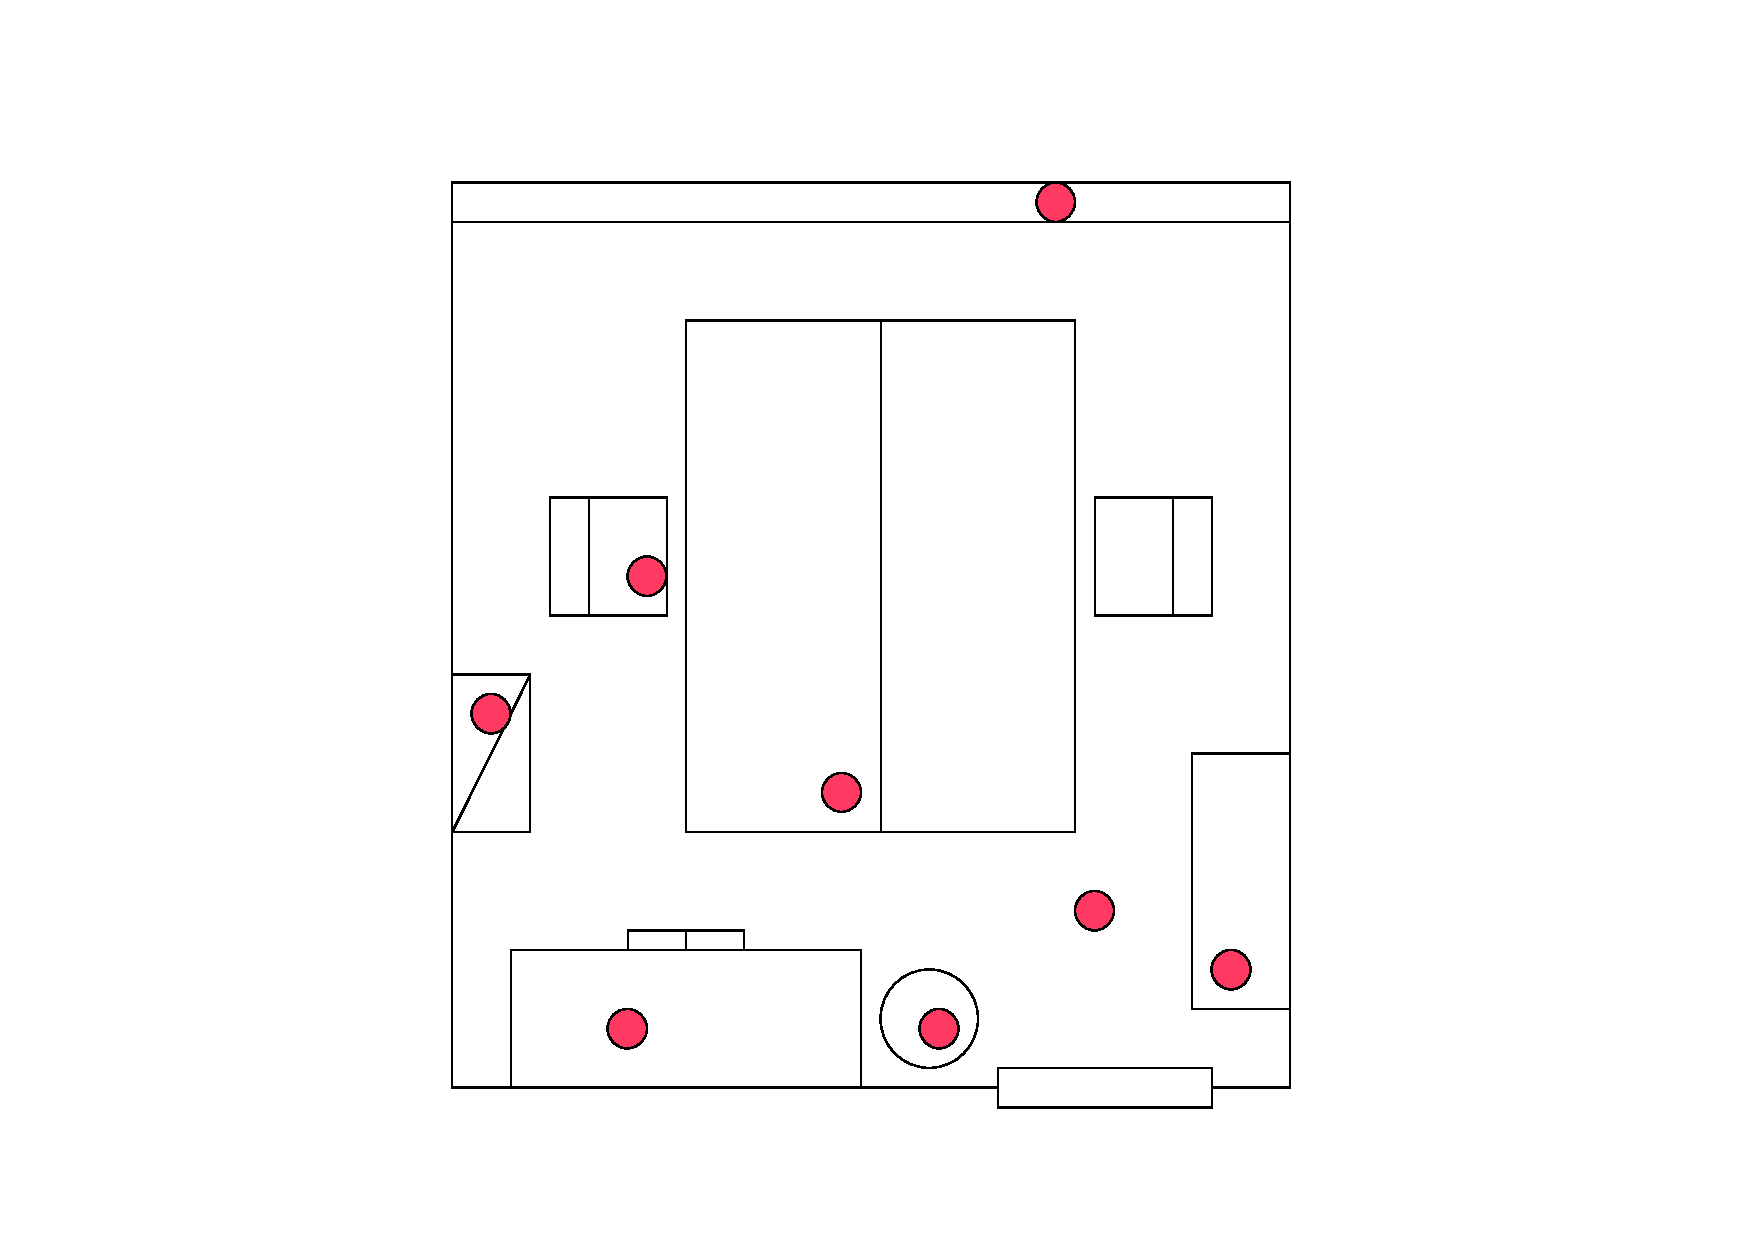
\includegraphics[height=1.35in,height=1.7in]{office.pdf}
  	}
	\\
\subfloat[]{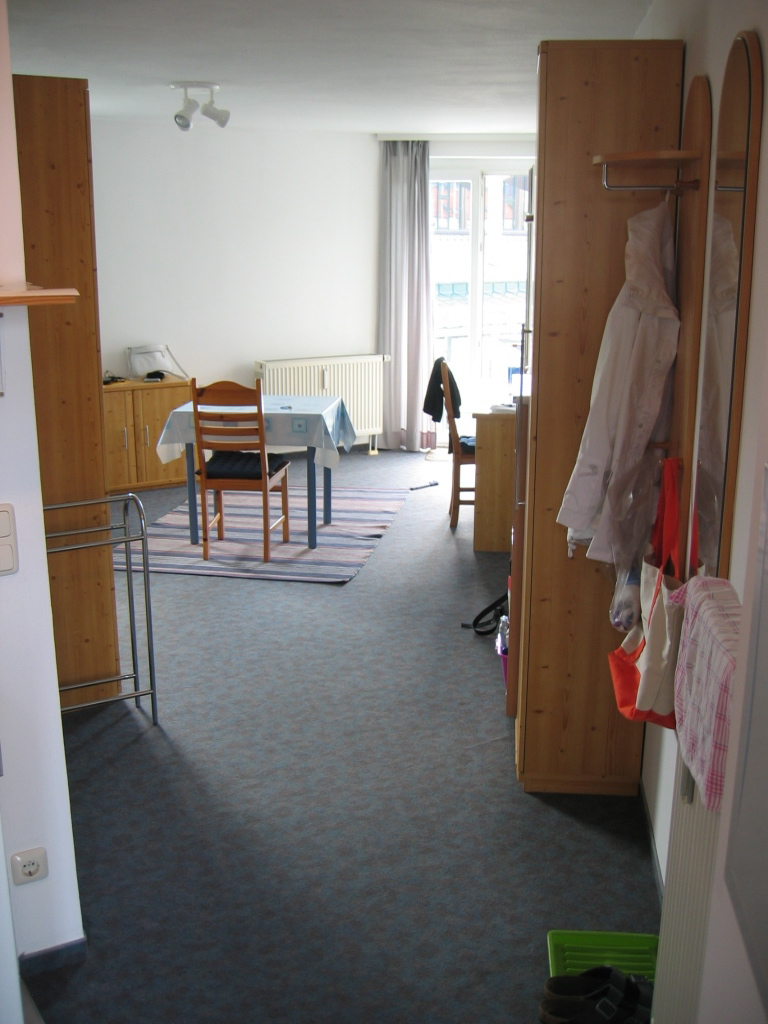
\includegraphics[height=1.35in,height=1.7in]{room.jpg}
  	\label{fig:room}}
\subfloat[]{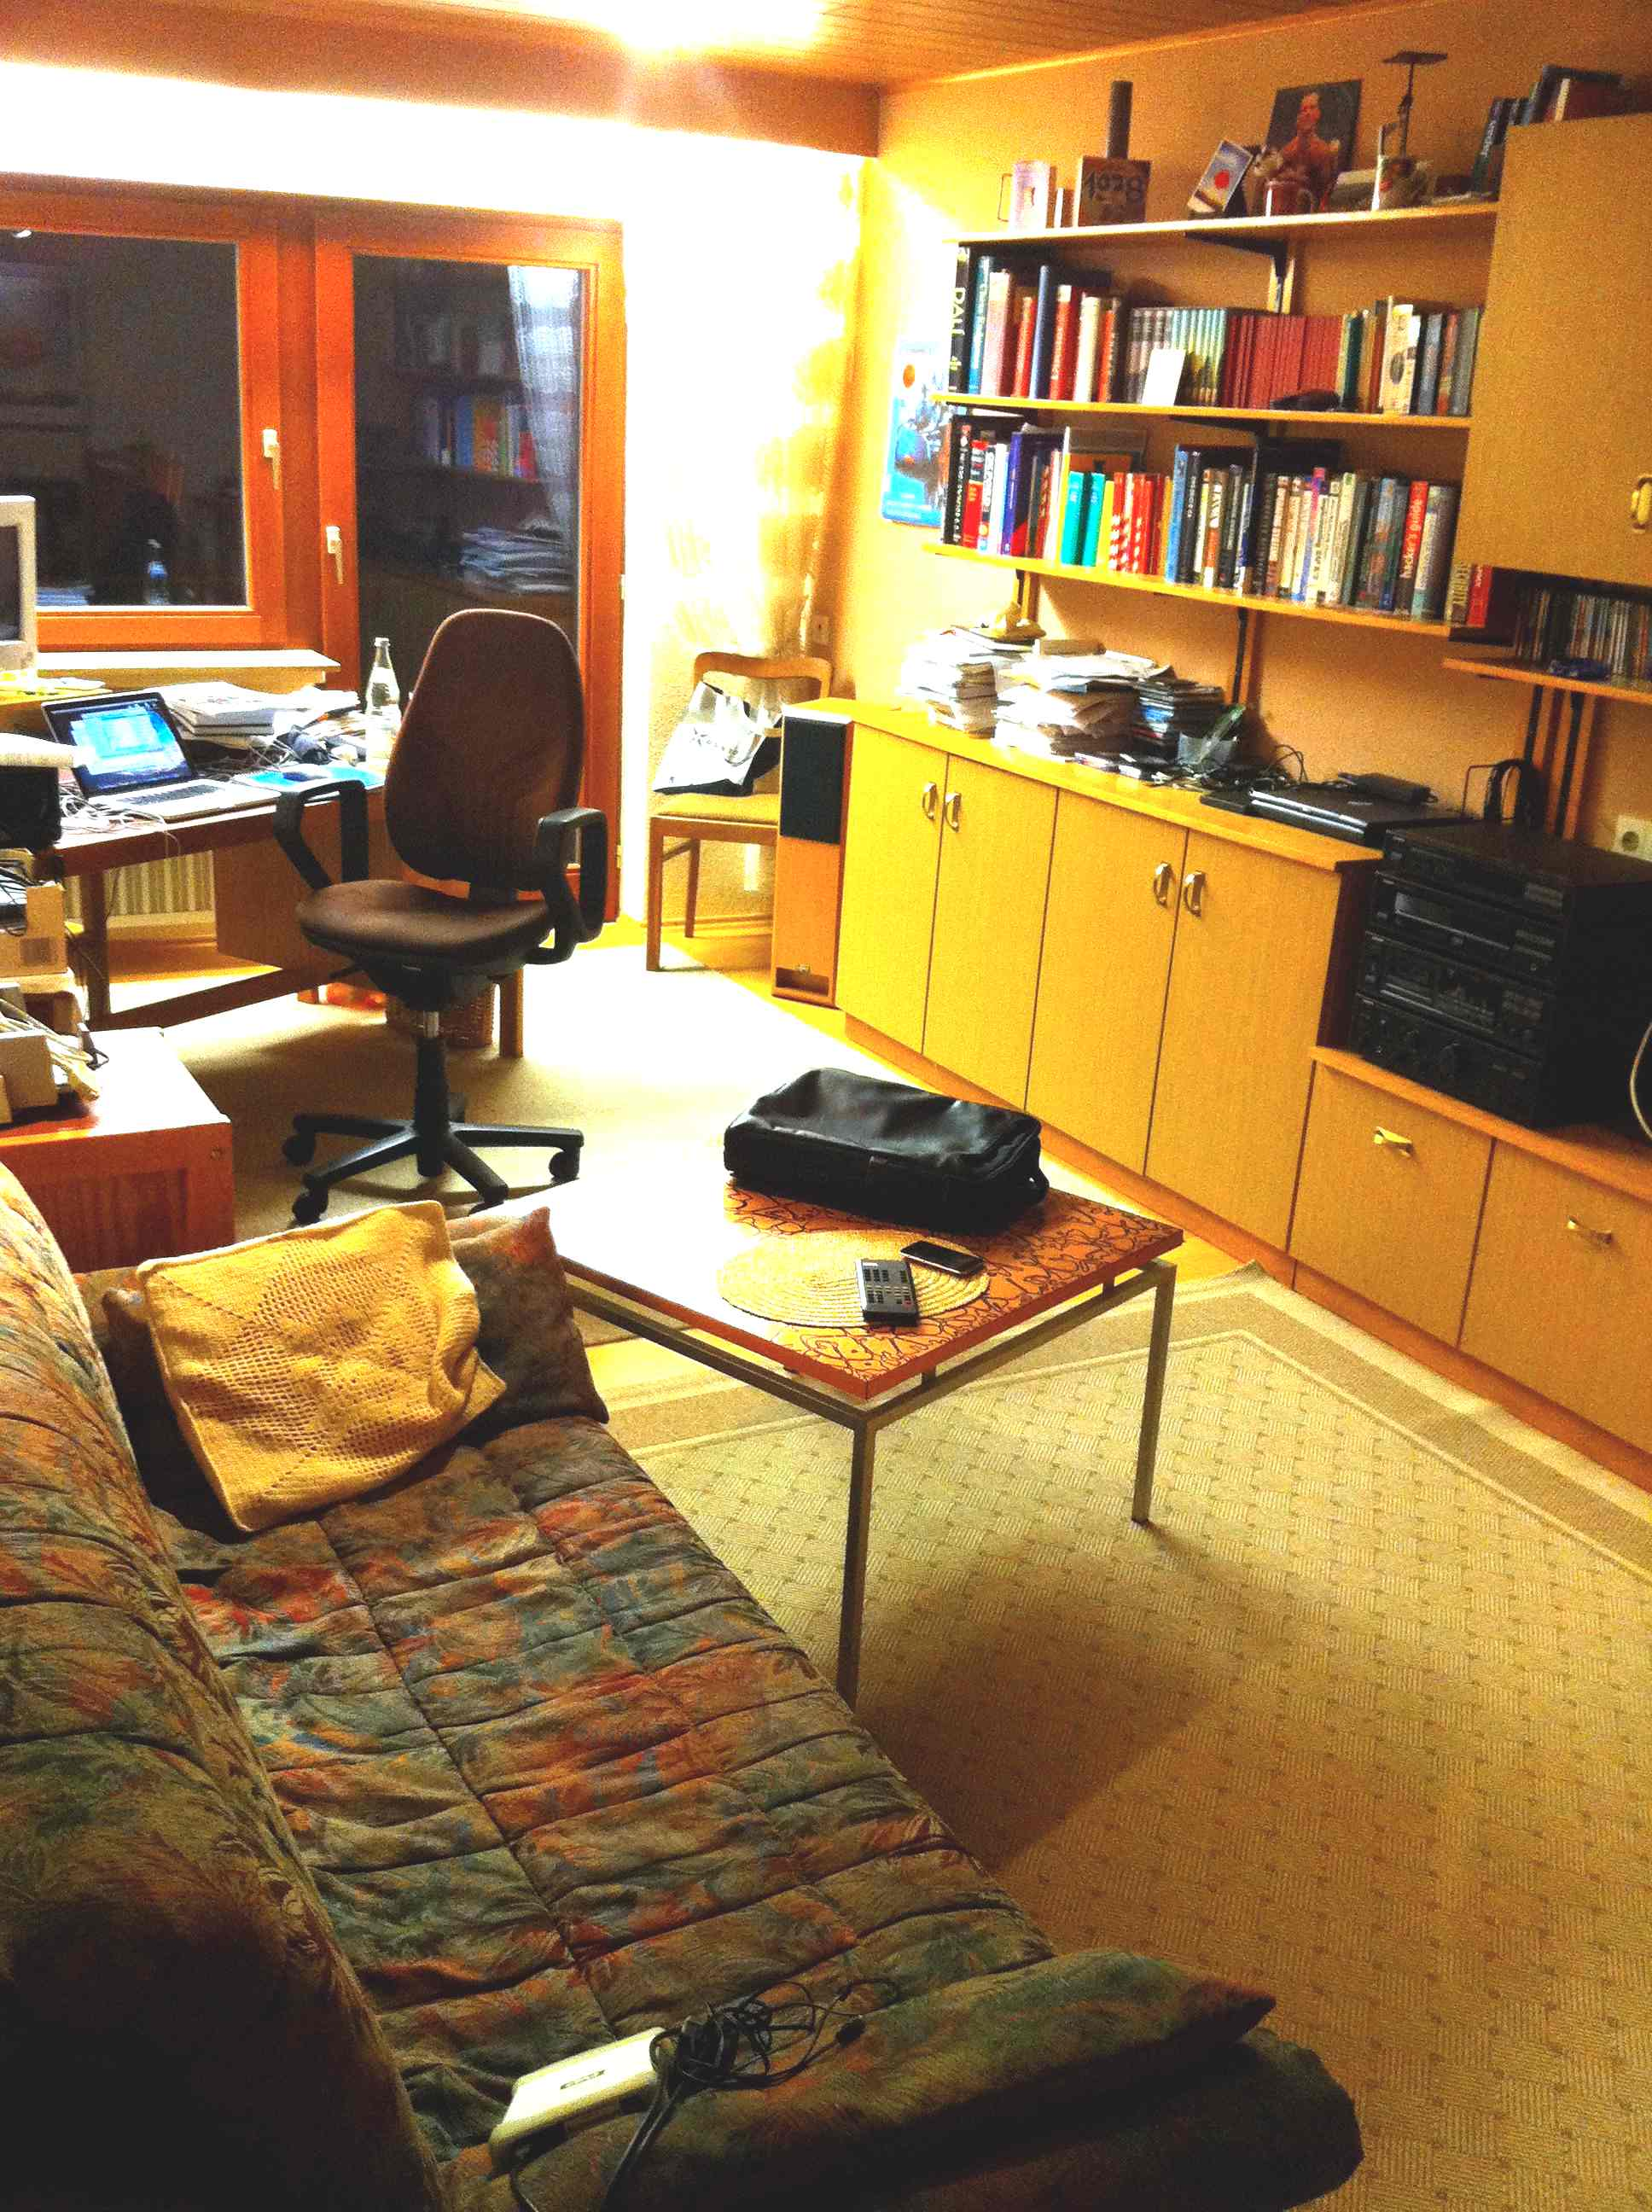
\includegraphics[height=1.35in,height=1.7in]{home.jpg}
  	\label{fig:home}}
\subfloat[]{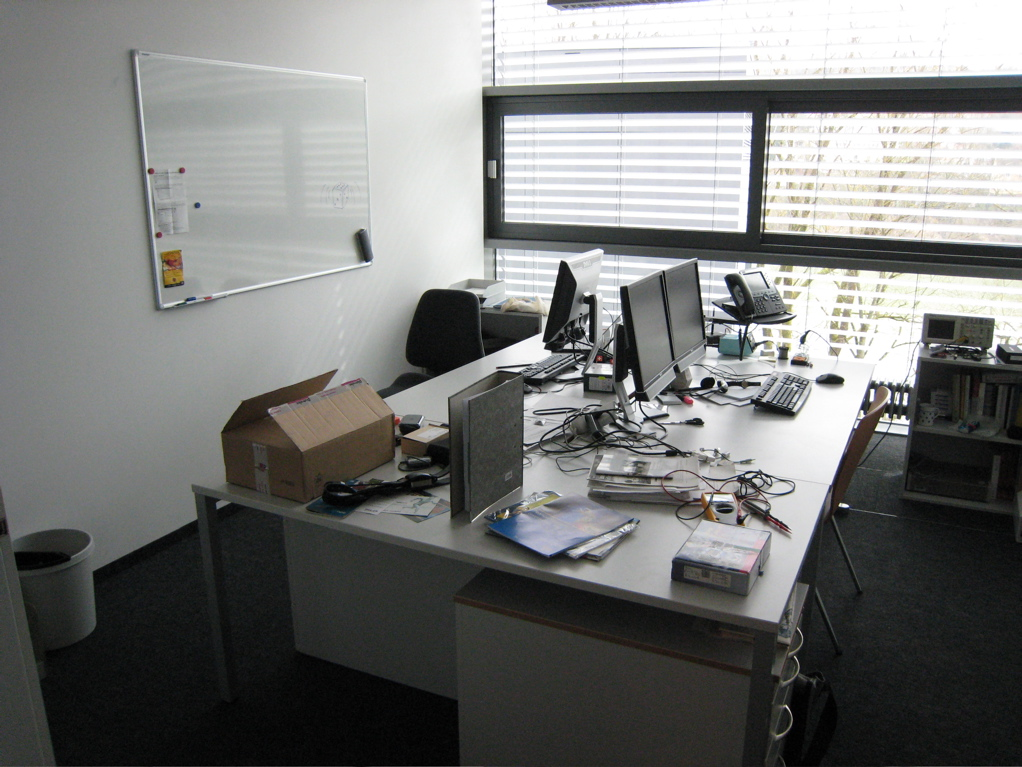
\includegraphics[height=1.35in,height=1.7in]{office.jpg}
  	\label{fig:office}}
   \end{center}
\vspace{-10pt}
\caption[Experiment environment]{The top figures show schematics of the rooms used for the experiments. 
The symbolic locations we try to detect are marked in red for the apartment living room and office. 
Below the schematics there are actual photos from the locations.}
\label{fig:experiment}
\end{figure} 


\section{Experimental Validation}
\label{sec:experimental}
During the evaluation, we design and conduct experiments for both modes of our method,
specific and abstract location. We always introduce the details to the specific location mode first,
going into details about the scenario and procedure.

%An important concern in the design of the experiments was to work with
%realisti scenarios and not only demonstrate where our method works,
%but also show where are the limits.

\subsection{Validation Scenarios}
\subsubsection{Specific Location Mode}
As basis for our study, we pick three scenarios: 
an office, a living room, and a
one room student apartment. In each scenario a set of obvious locations
for placing objects are selected. These include the
furniture present in the room (both open such as table or sofa and
closed such as cupboards), the floor, the window ledges and additional
objects such as the stereo. In the
office scenario we also include three pockets (two different
pockets of a jacket and a jeans pocket), the inside of a backpack
and a suitcase as well as a trashcan. 
A full listing of the investigated location is given in
Table~\ref{table:location} and illustrated in
Figure~\ref{fig:experiment}. There are 16 locations in the
office, 9 in the living room and 10 in the apartment (total of 35).


We record 30 experimental runs on each specific location (a total of
over 1000 events), each time randomly varying the exact position of the recording. 
The object is placed according to positions drawn randomly from a uniform distribution.
Of the 30 runs, 10 are randomly picked to train the classifiers, the remaining 20 are
used as test set. Evaluation is performed
first on each individual scenario (assuming that room level
location could be obtained by other means). We also perform an evaluation on a data set containing all
locations from the three scenarios, to see how our method
behaves when the number of locations increases.

\begin{table}[ht]
 \caption[Symbolic locations picked for the experiments]{Chosen symbolic locations and abstract location classes. 
The letter in front is the identification
 for the individual confusion matrix plots presented later in the paper. The letter in brackets behind the class description, is the
 identifier for the confusion matrix plot over all 35 locations. In j. , o. j. and tr. pocket stand for inside jacket, outside jacket and trousers pocket. }
\scalebox{0.82}{
\begin{tabularx}{75pt+\textwidth}{lllll}
\toprule
Office& &Living room&Apartment&Surfaces\\
\midrule
a. backpack(a)&k. in j. pocket(C) & a. desk(h)& a. bath carpet(f)& a. polster open\\
b. cupboard(z)&l. tr. pocket (e)& b. floor(u)  & b. bed(p)&b. glass open\\
c. suitcase(w)&m. cartbox (F) & c. sofa(n)& c. chair(b)& c. iron open\\
d. drawer(t)& n. ledge (H) &d. table(A)& d. desk (wood) (l)& d. stone closed\\
e. desk(D)& o. chair (v) & e. chair(c)&e. radiator(d)& e. wood closed\\
f. top drawer(E)&f. drawer (m)& f. ledge(k)& f. glass closed\\
g. cabinet (x)& p. shelf (i) &g. ledge (G)& g. carpet floor(B)& g. iron closed\\
h. o j. pocket(j) & & h. stereo (s)& h. cupboard(g)& h. metal open\\
i. trashcan(I)& & i. tv (j)& i. drawer(q)& i. polster closed\\
j. carpetfloor(r)& & & j. wardrobe (o)& j. stone open\\
\bottomrule 
\end{tabularx}}
\label{table:location}
\end{table}

\subsubsection{Abstract Location Type Mode}
The abstract location types are defined according to the surface
material and the location being open (e.g. a table) or closed (e.g a
cabinet or a drawer). As shown in Table \ref{table:location} this
lead us to 9 classes including most typical surfaces (wood, glass
metal, stone, cushion). To get a sufficient number of different instances
for each class we record the data in a furniture store. For
every abstract class we pick 6 different pieces of furniture. Two
recordings are conducted on each specific piece of furniture leading to 9
data points per abstract class and a total of 144 events. For the
evaluation two pieces from each class (four events per
class) are picked for training and 4 (8 events per class) are
retained for testing. This is consistent with the envisioned
application use case in which the user would be given a device "factory 
pre-trained" for each class and use it to recognize instances of the
class not seen by the system before. 

\subsection{Experimental Procedure}

\subsubsection{Setup}


\begin{figure}[t]
\centering  
 \subfloat[]{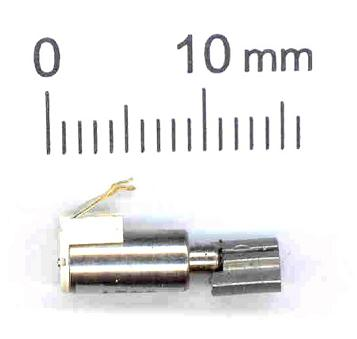
\includegraphics[trim=10 0 10 0,clip,height=1.9in]{vibmot.jpg}
  	\label{fig:vibmot}}
  \subfloat[]{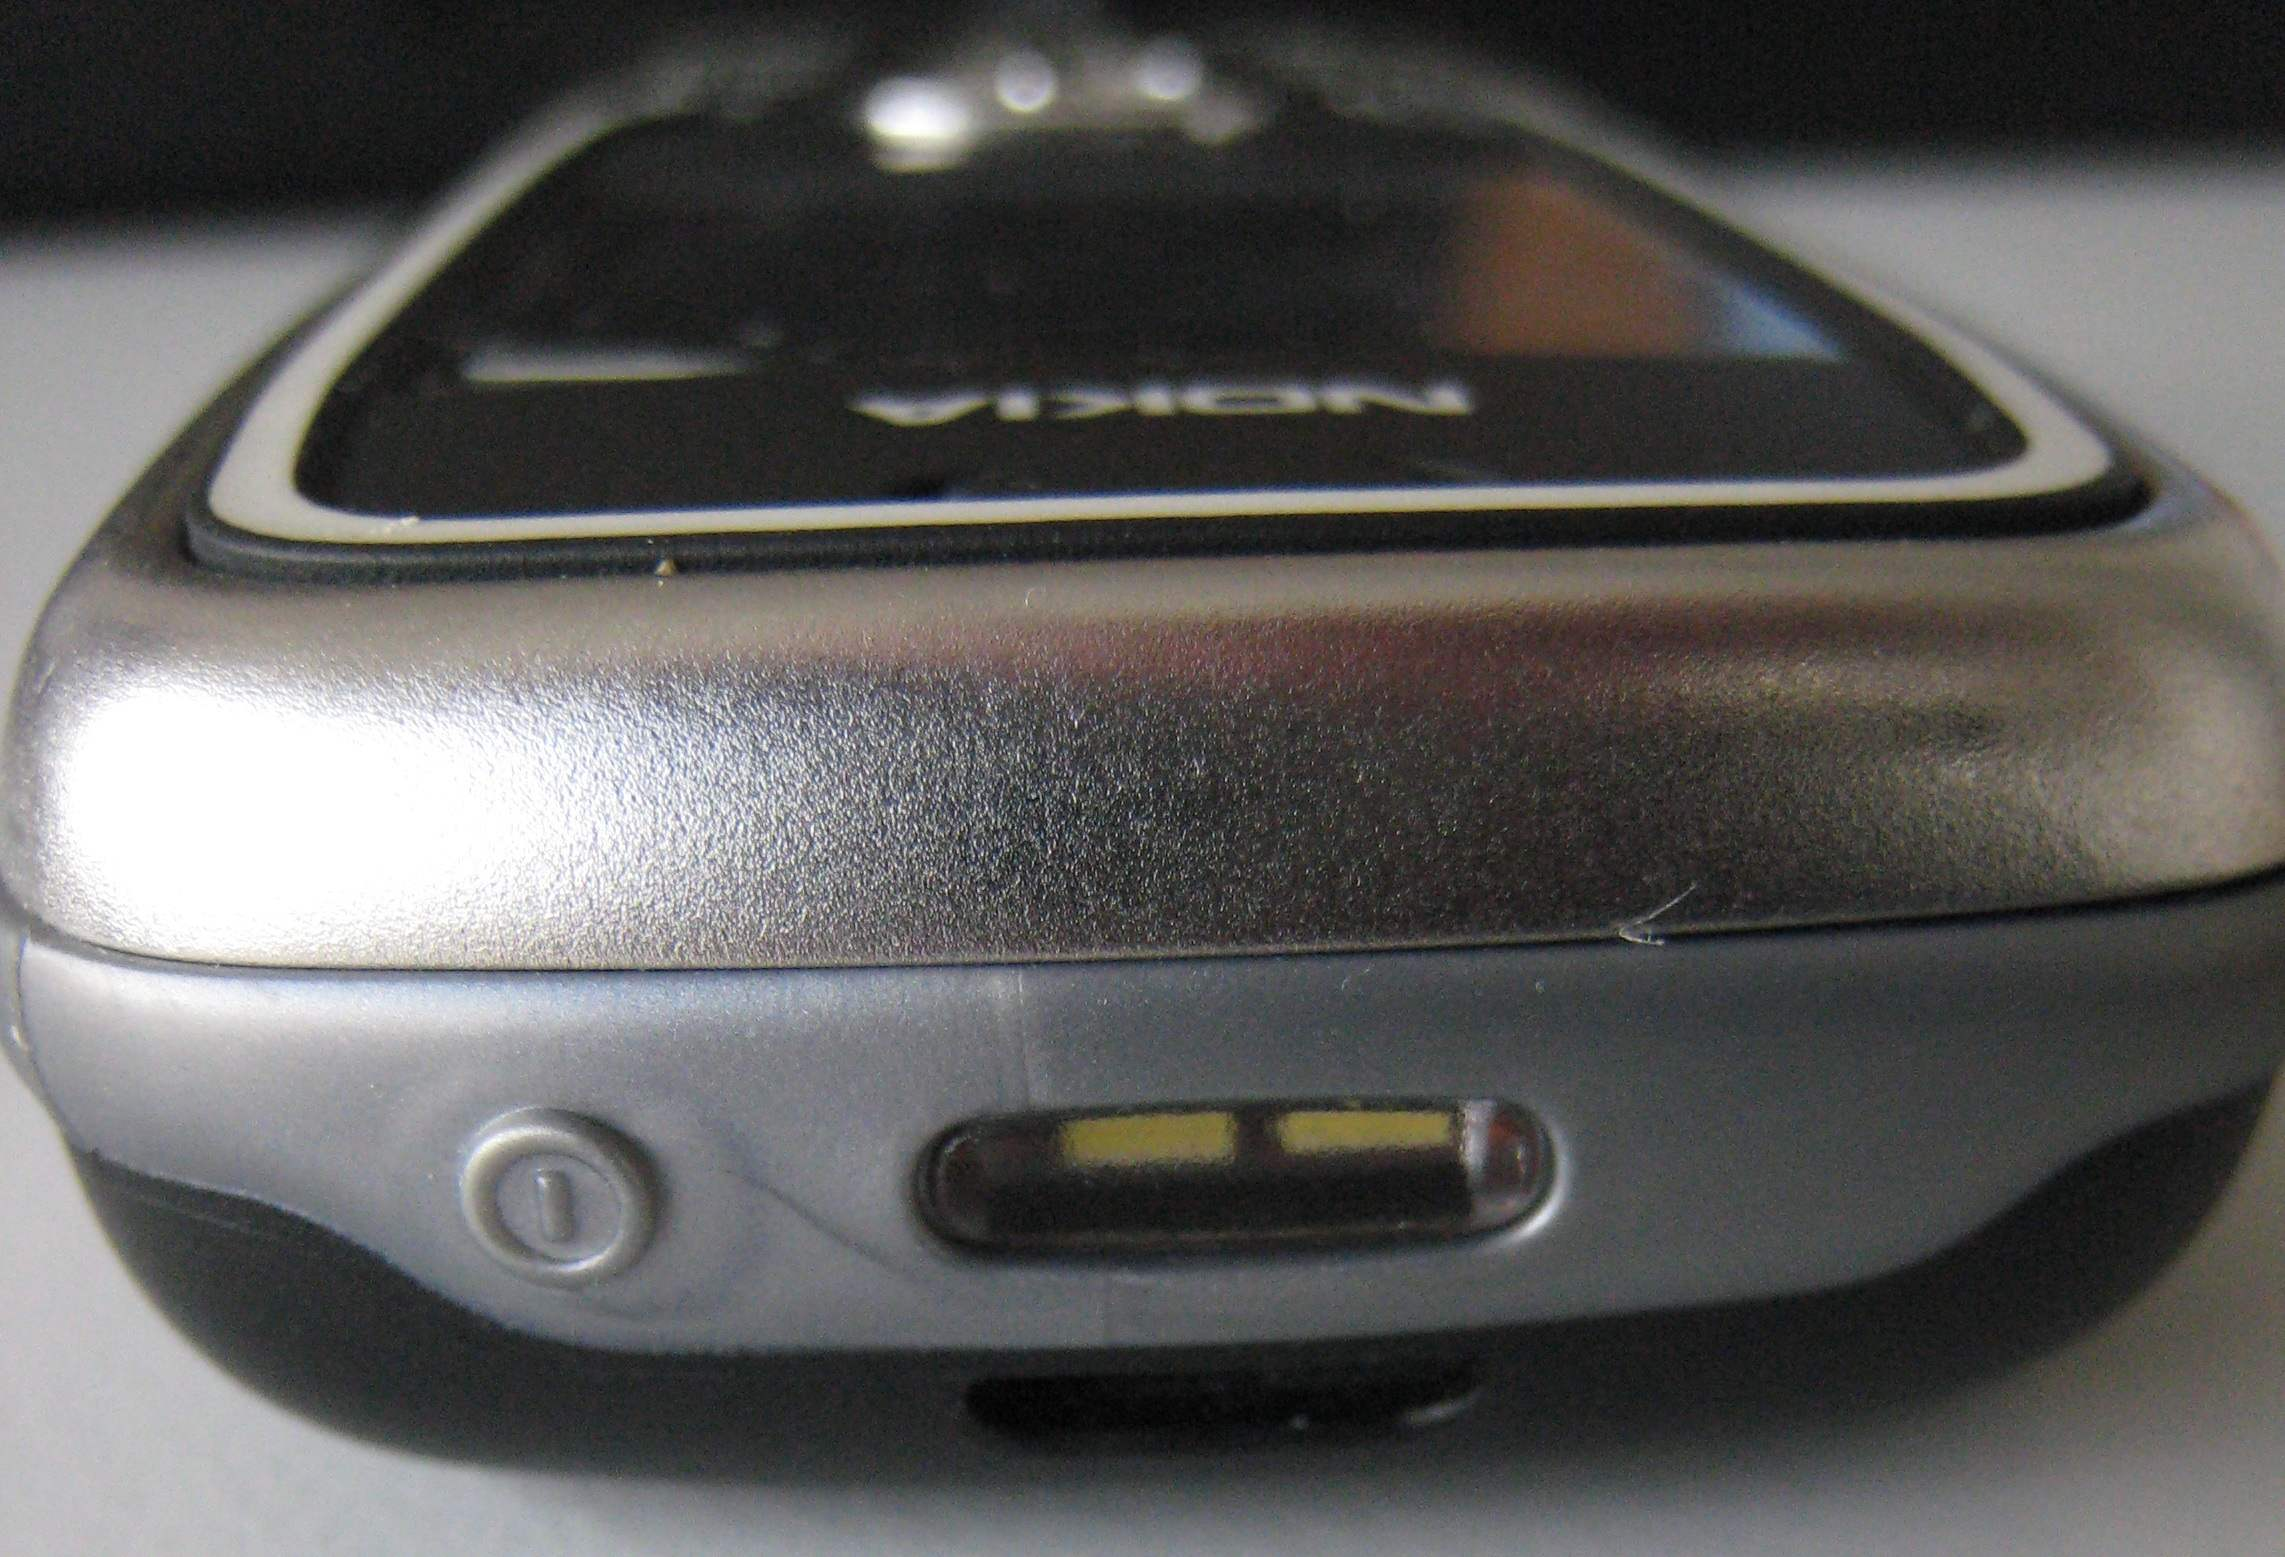
\includegraphics[height=1.35in,height=1.9in]{speaker.jpg}
  	\label{fig:speaker}}
\caption[Vibration motor and phone loudspeaker]{A picture of a common vibration motor and the extra loudspeaker on the Nokia 5500 Sport.}
\label{fig:hardware}
\end{figure}
For the experiments, we use the Nokia 5500 Sport, see Figure~\ref{fig:hardware}. It is a mobile phone of Nokia's third S60 series, equipped with an accelerometer and an extra loudspeaker. The mobile is able to run C++, Java and python code. We record data using python.
The evaluation is done in batch processing using a mixture of Python, Matlab scripts and Java code, mainly consisting of the Weka machine learning package.

\begin{figure}[t]
  \begin{center}
  \subfloat[]{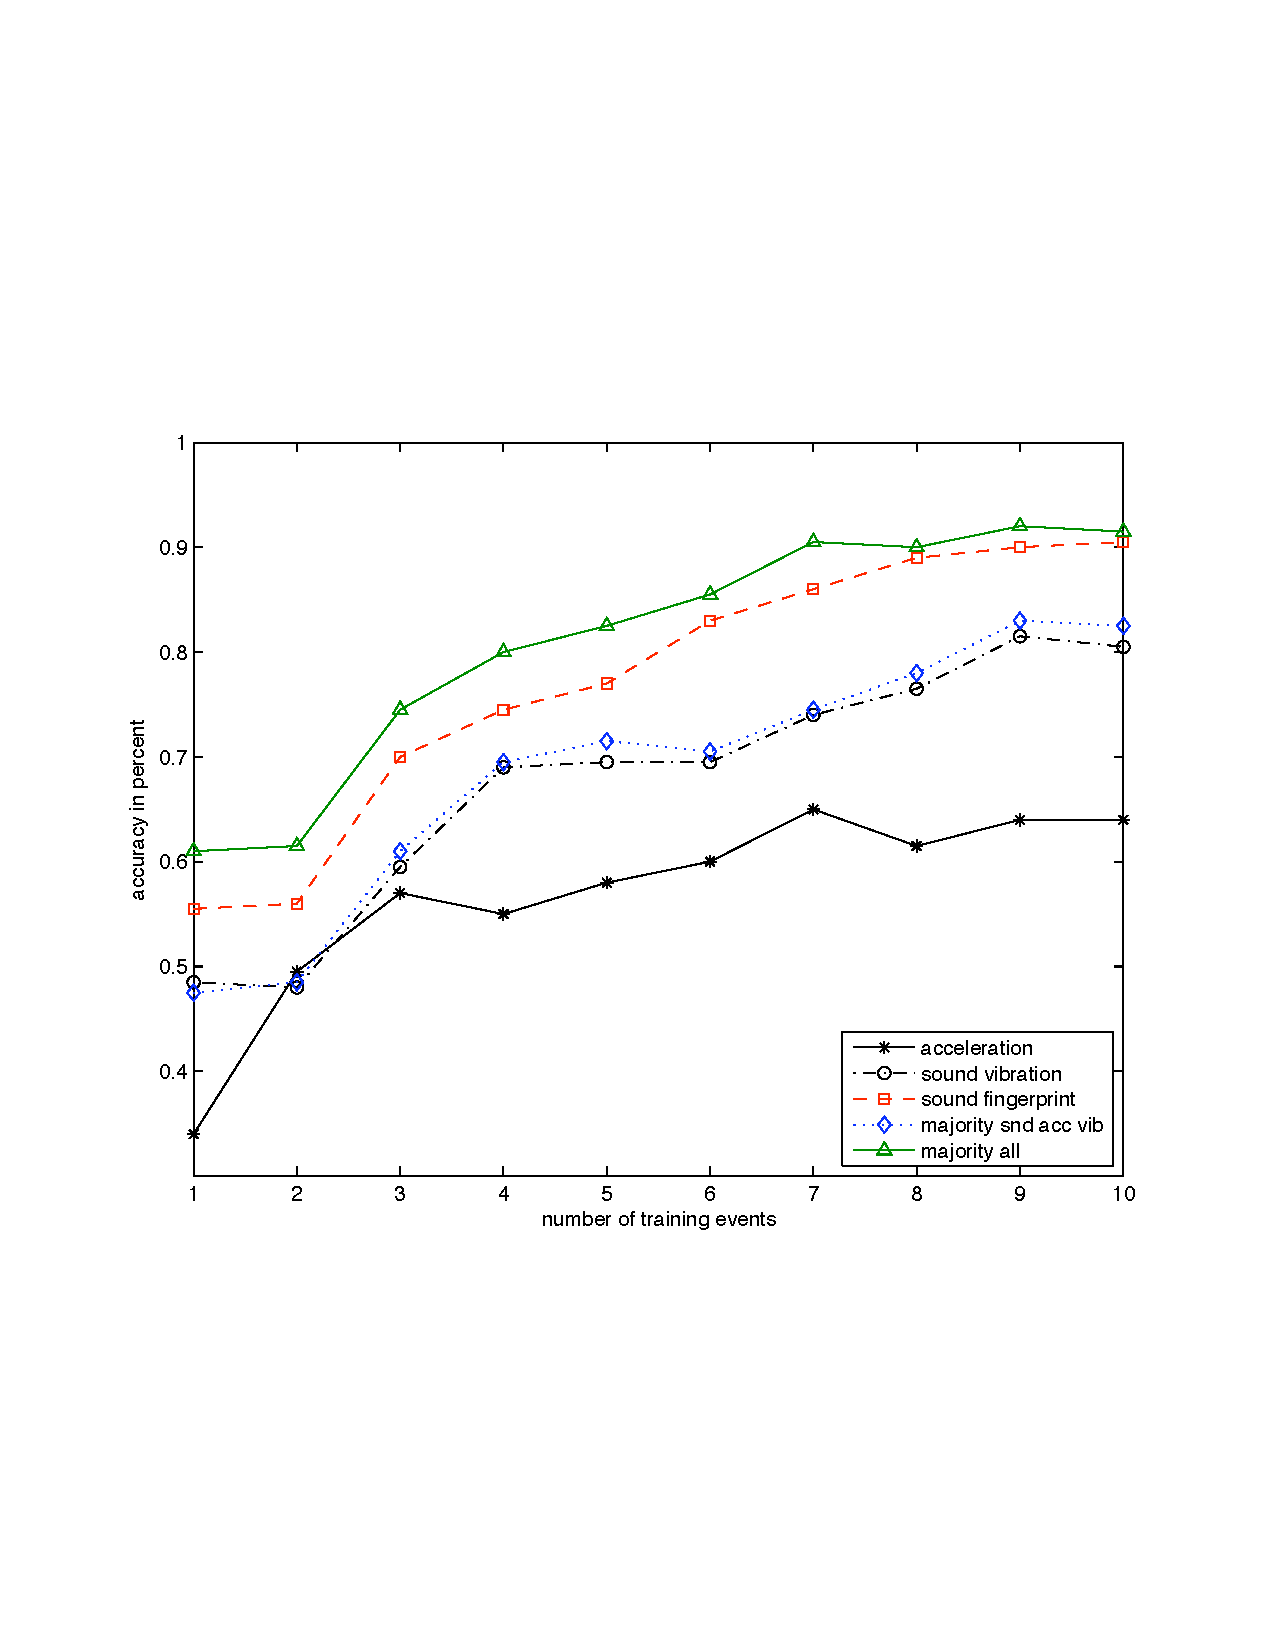
\includegraphics[trim=10 0 10 0,clip,height=2in]{appartmenttraining.pdf}
  	\label{fig:apptraining}}
\subfloat[]{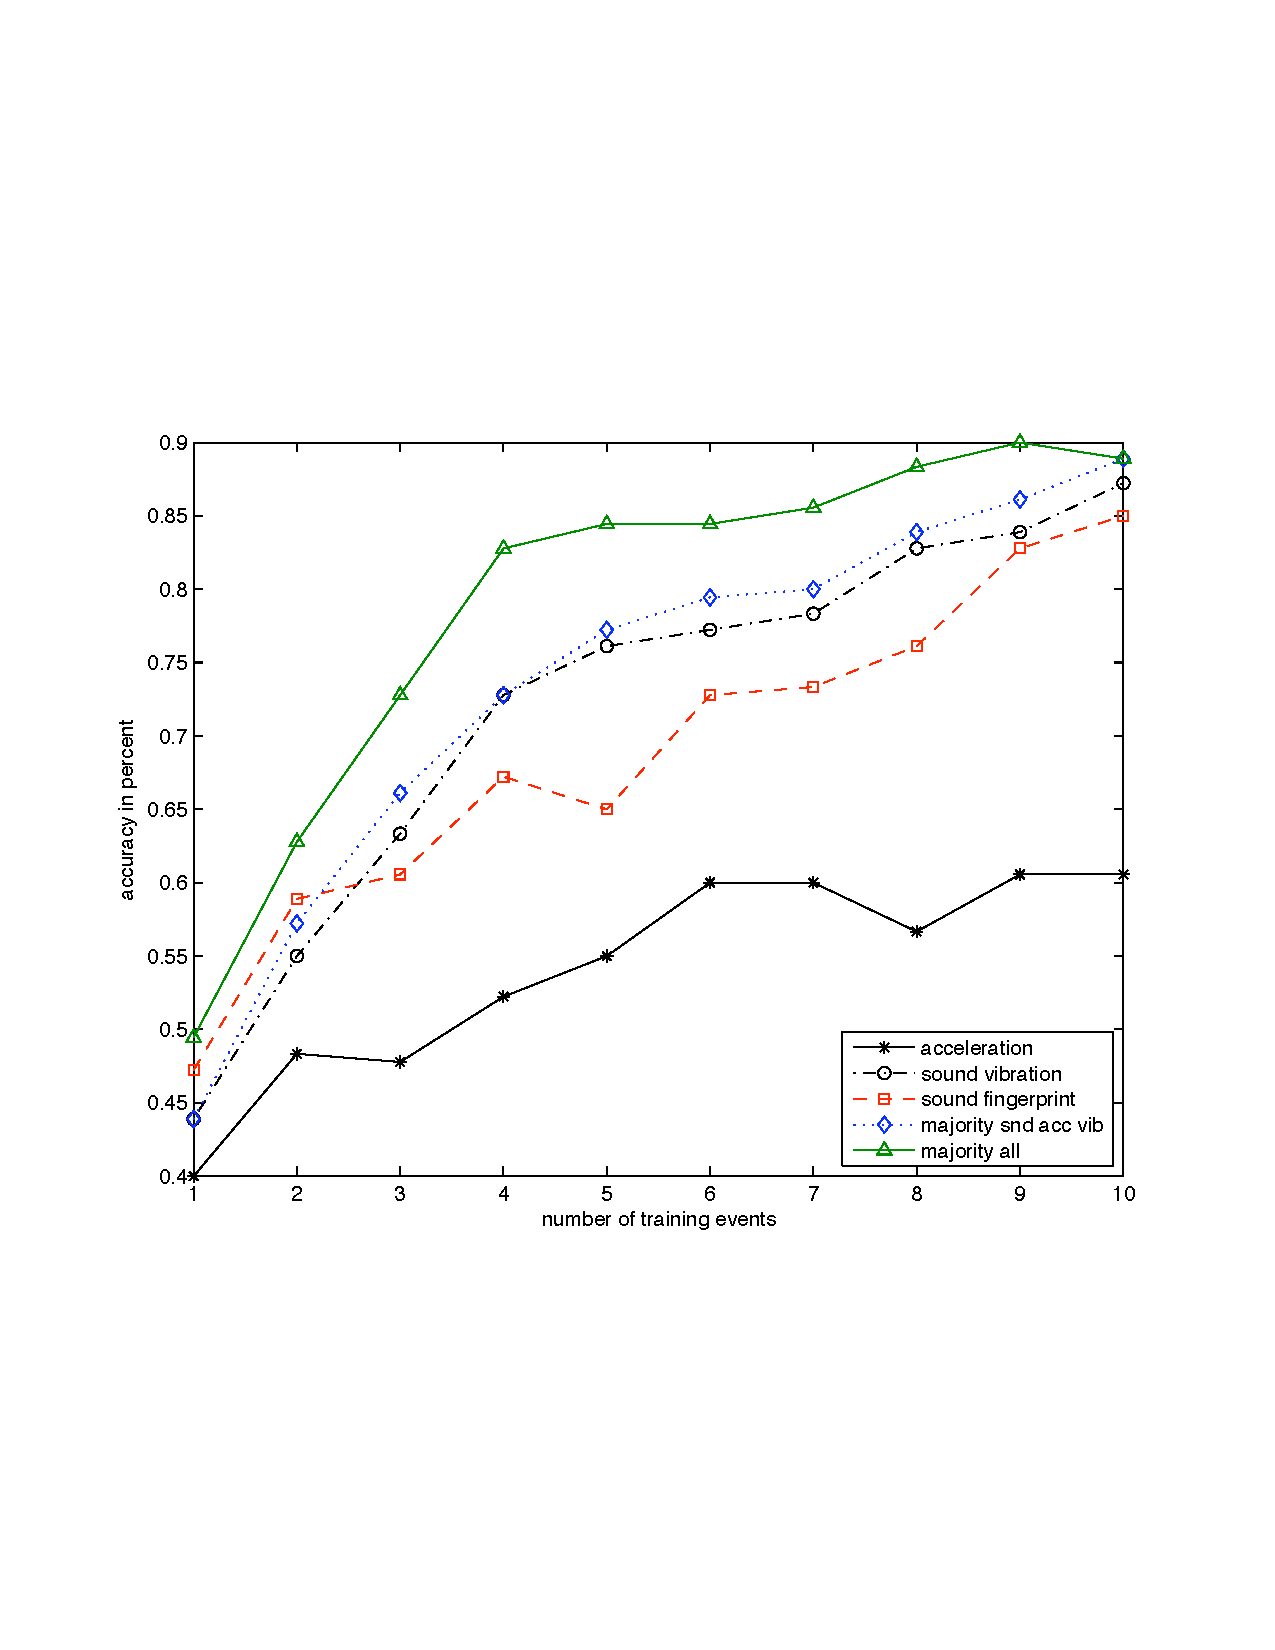
\includegraphics[trim=10 0 10 0,clip,height=2in]{livingroomtraining.pdf}
  	\label{fig:livingtraining}}
	
	
  \subfloat[]{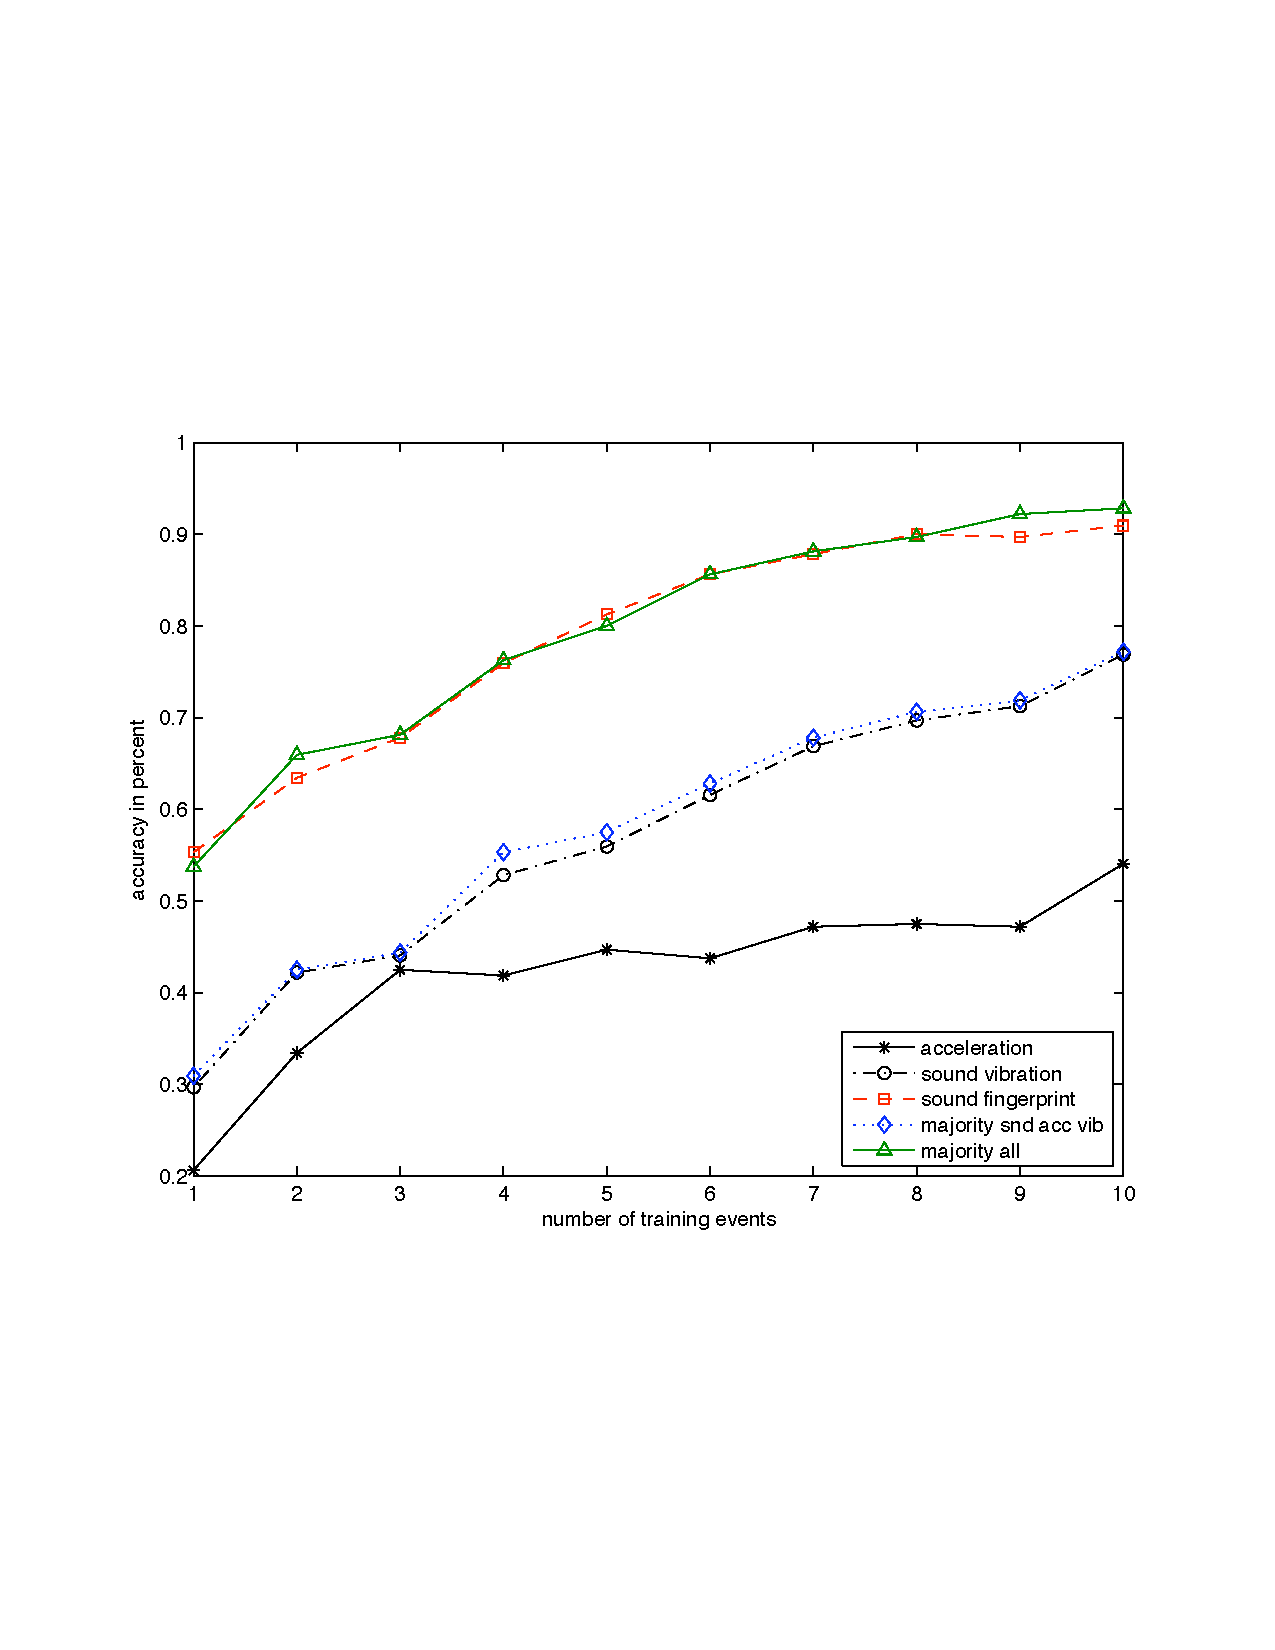
\includegraphics[height=1.35in,height=2in]{officetraining.pdf}
  	\label{fig:officetraining}}
   \end{center}
\caption[Accuracy versus training samples]{ The classification accuracy depending on the number of training events and different sensing modalities for the appartment \subref{fig:apptraining}, 
living room \subref{fig:livingtraining}, and office scenario \subref{fig:officetraining}.}
\label{fig:training}
\end{figure} 


\subsubsection{Data Acquisition}
An experimental run consists of the following steps. First the phone
is placed on a random spot on a particular location. Using a uniform
distribution, the actual spot is determined randomly. Then the
measurement is started. While the mobile vibrates for 5 sec. lying
face up on the surface, the sound from the phone
vibrating is sampled by the on-board microphone with 8
kHz and the acceleration with 30 Hz. After the vibration measurement
is done the mobile plays the sound sample consisting of 8 beeps in
distinct frequencies from 500 to 4000 Hz in 500 Hz steps (as seen in Figure~\ref{fig:soundfing}). Each tune is
1 sec. long. While the mobile plays this using the extra loudspeaker,
the python script records the sound with 8000 Hz over the built-in
mobile microphone. The loudspeaker faces the surface, as depicted in
Figure~\ref{fig:hardware}. We get around a problem of accessing
full-duplex mode in python on the Nokia phone by using the music
player and the extra speaker.


\begin{figure}[t]
  \begin{center}
  \subfloat[]{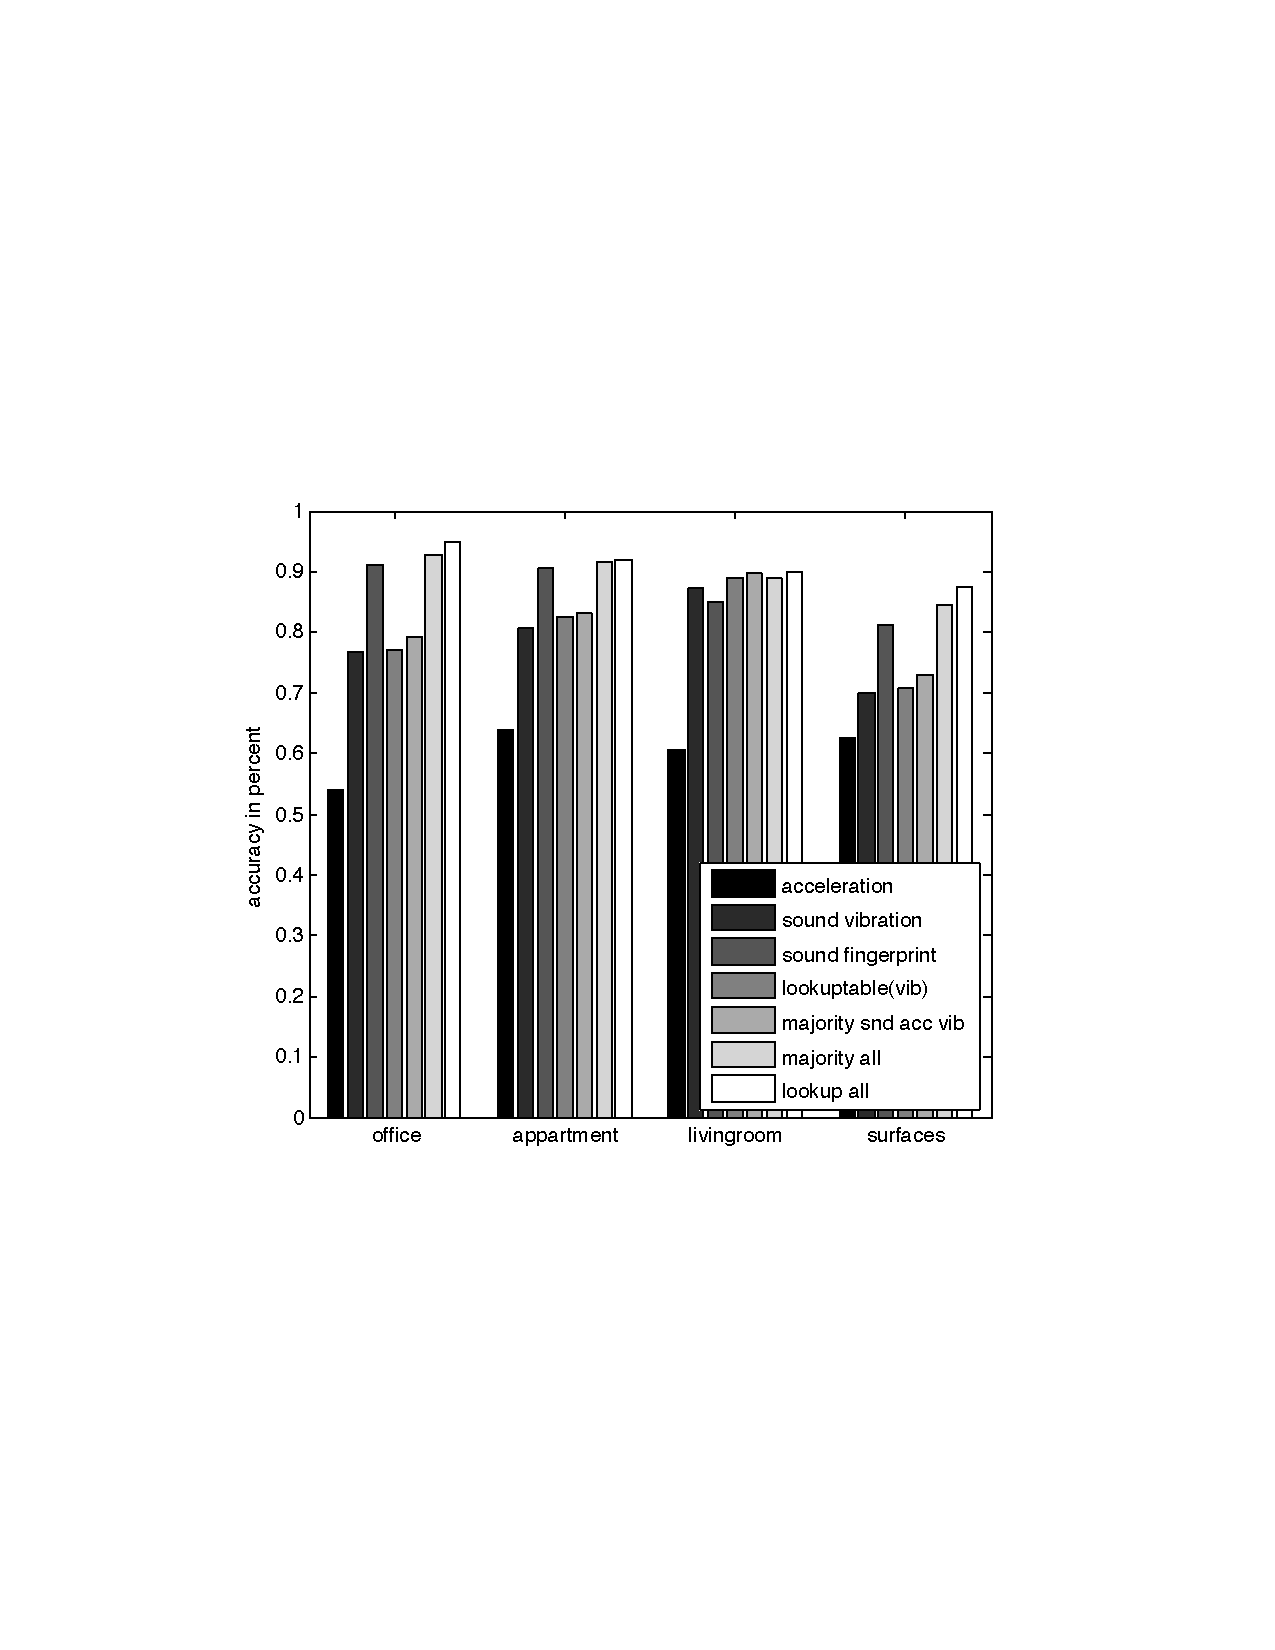
\includegraphics[trim=10 0 10 0,clip,height=1.8in]{barchart1st.pdf}
  	\label{fig:barchart1}}
  \subfloat[]{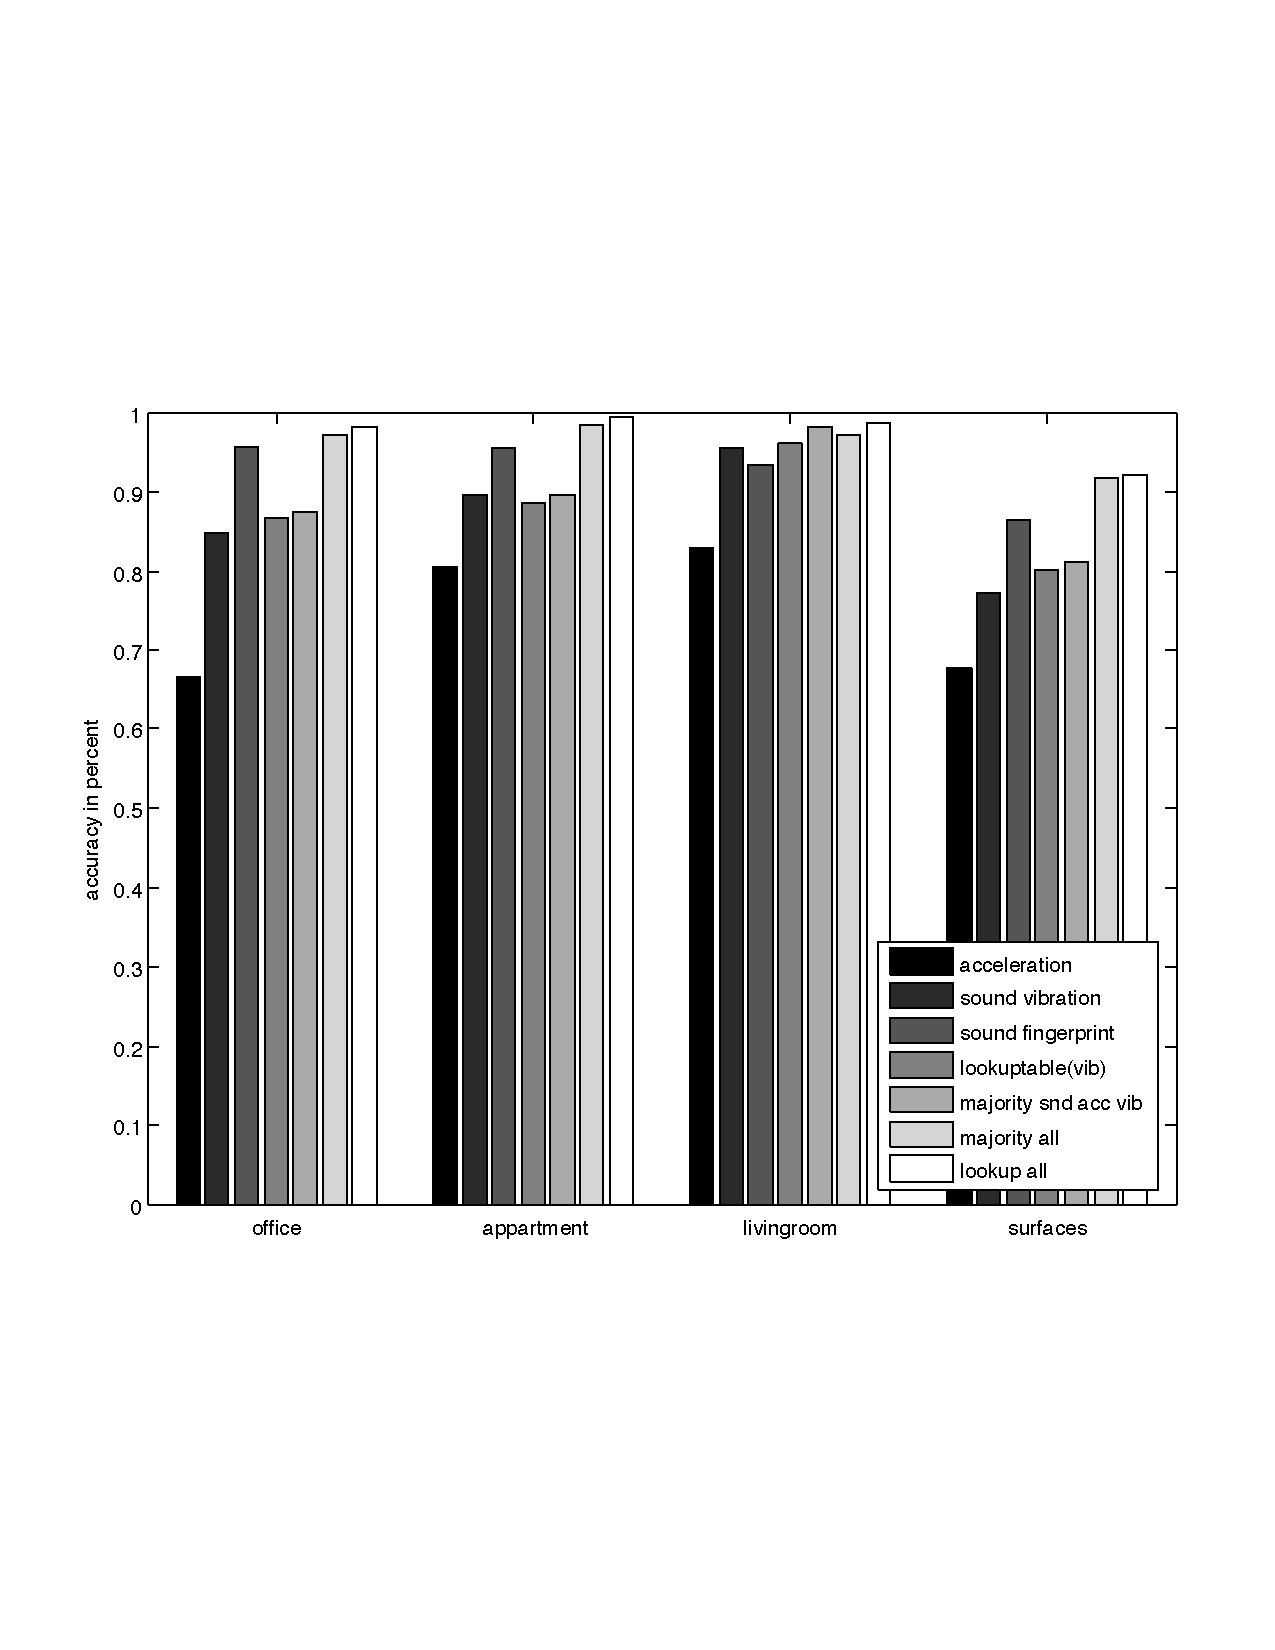
\includegraphics[height=1.35in,height=1.8in]{barchart2nd.pdf}
  	\label{fig:barchart2}}
   \end{center}
\caption[Classification performance per scenario]{ Barcharts for living room, office, apartment, and abstract
 classes using just the first result of the
 classification~\subref{fig:barchart1} and allowing the 2nd best
 vote~\subref{fig:barchart2}}

\label{fig:barcharts}
\end{figure} 



\begin{figure}[t]
\centering  
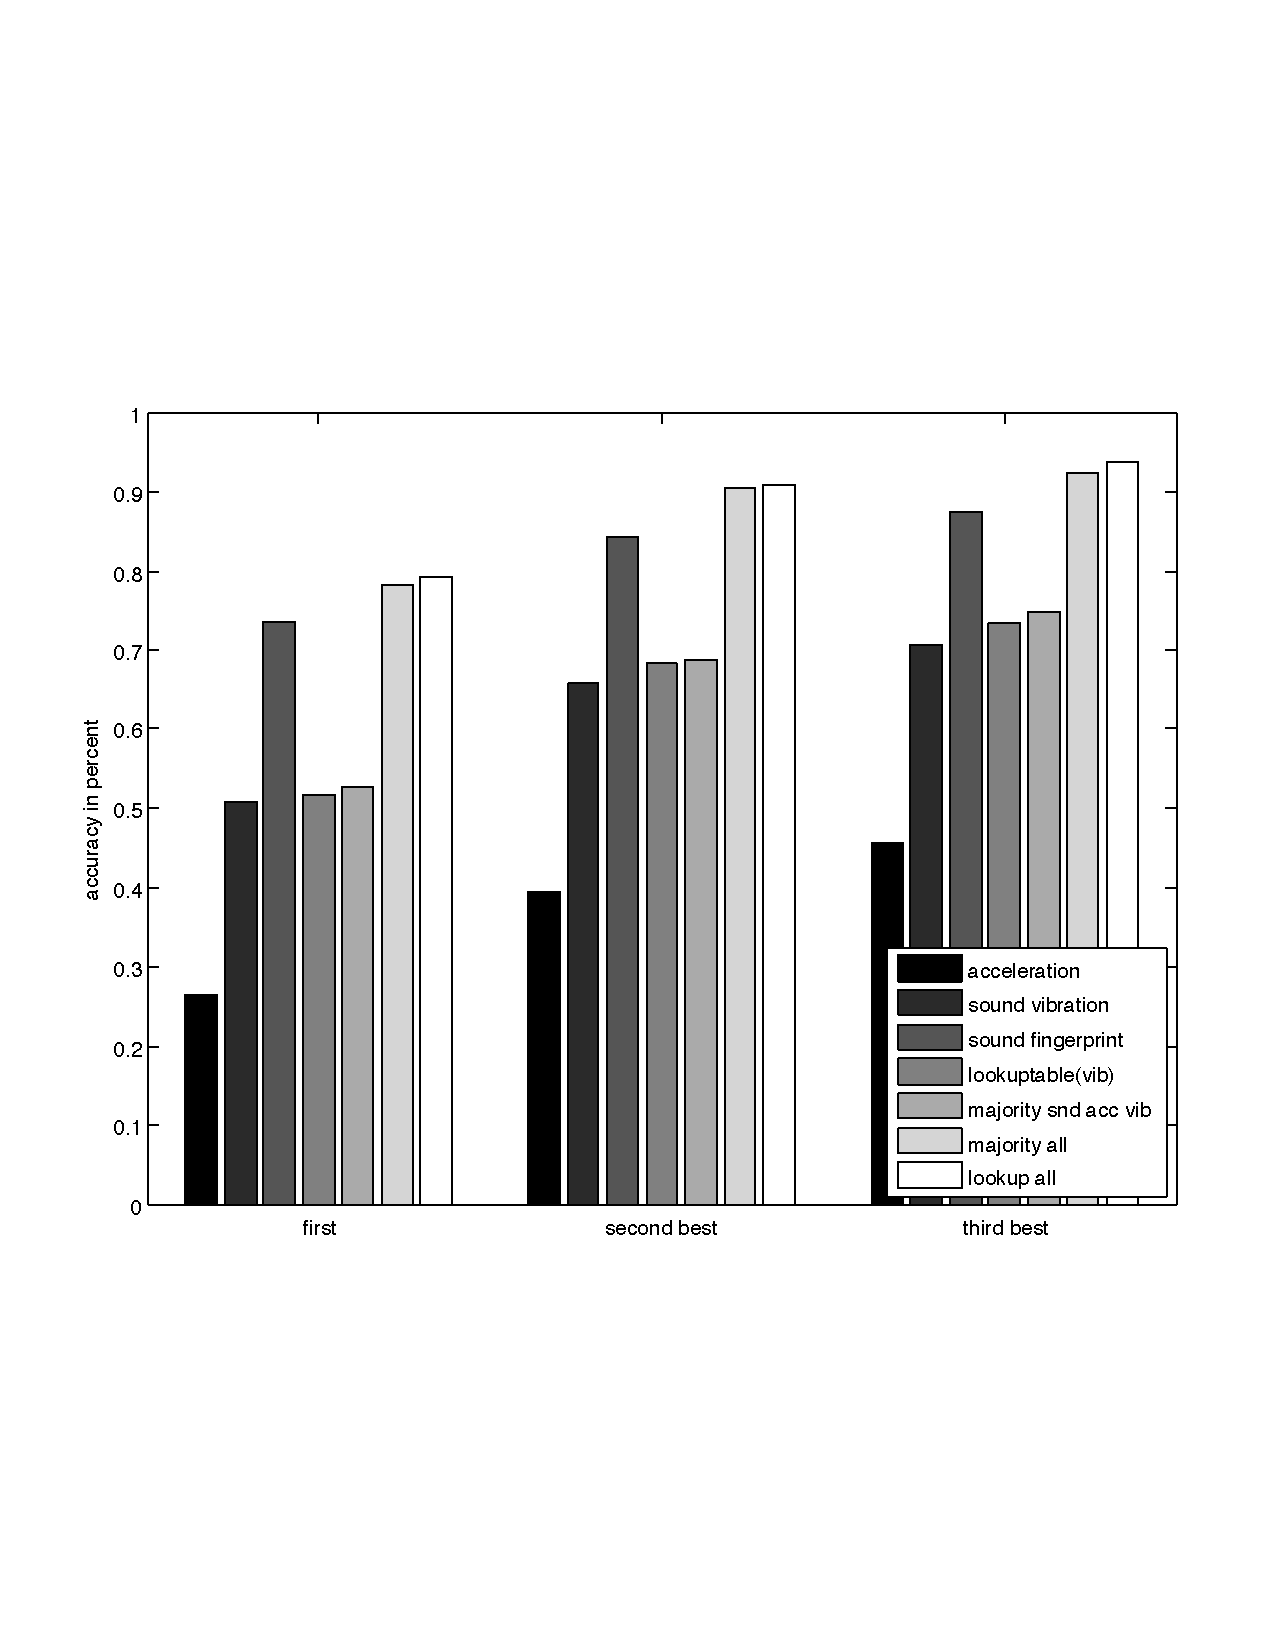
\includegraphics[scale=0.36]{barchartall.pdf}
\caption[Classification performance over all]{Barchart for office living room, apartment and all combined
 including 1st 2nd 3rd best} \label{fig:barchart3} \end{figure} 



\subsection{Experimental Results} \label{sec:results}

The recognition performance for different scenarios, experiments and 
recognition modalities are summarized in
Figure \ref{fig:barchart1} for the three individual scenarios of
the specific location mode and the abstract location class and
in Figure \ref{fig:barchart2}, combining all 3 locations and second/third best voting.
Additionally, examples of confusion matrices are visualized for the
office scenario, the combination of all three specific location mode
scenarios and the abstract location type mode in Figures
\ref{fig:conf1}, \ref{fig:all} and \ref{fig:confmasurf} respectively.
The dependency of the classification accuracy on the number of training events can be seen 
in Figure~\ref{fig:training} for the different scenarios.

In the more detailed discussion of the results given below and the
some of the figures we at times discuss "2nd best evaluation" or "3rd
best evaluation". This refers to cases where the correct class
is among the 2 or 3 first picks of the classification system. 



\paragraph{Office}
In the office scenario, 14 of the 16 locations can be classified with
near perfect accuracy. The single biggest confusion is between the
pocket on the inside of the jacket and the one on the outside. This
is plausible and to be expected. An unexpected result is the poor
recognition of the metal window ledge. It is confused with the
cart-box, the top shelf and the chair. 

The classification accuracy is 54\% using the event-based acceleration
classifier, 77\% for vibration sound, 91\% for the sound sampling,
77\% and 79\% for the vibration fusion cases. We reach up to 93-94\%
for the majority decision and lookup-table fusion using all
modalities. The sound sampling is the best non-fusion method with
91\%. The "2nd best evaluation" pushes the correct classified up to
96\%.

\begin{figure}[t]
  \begin{center}
  \subfloat[]{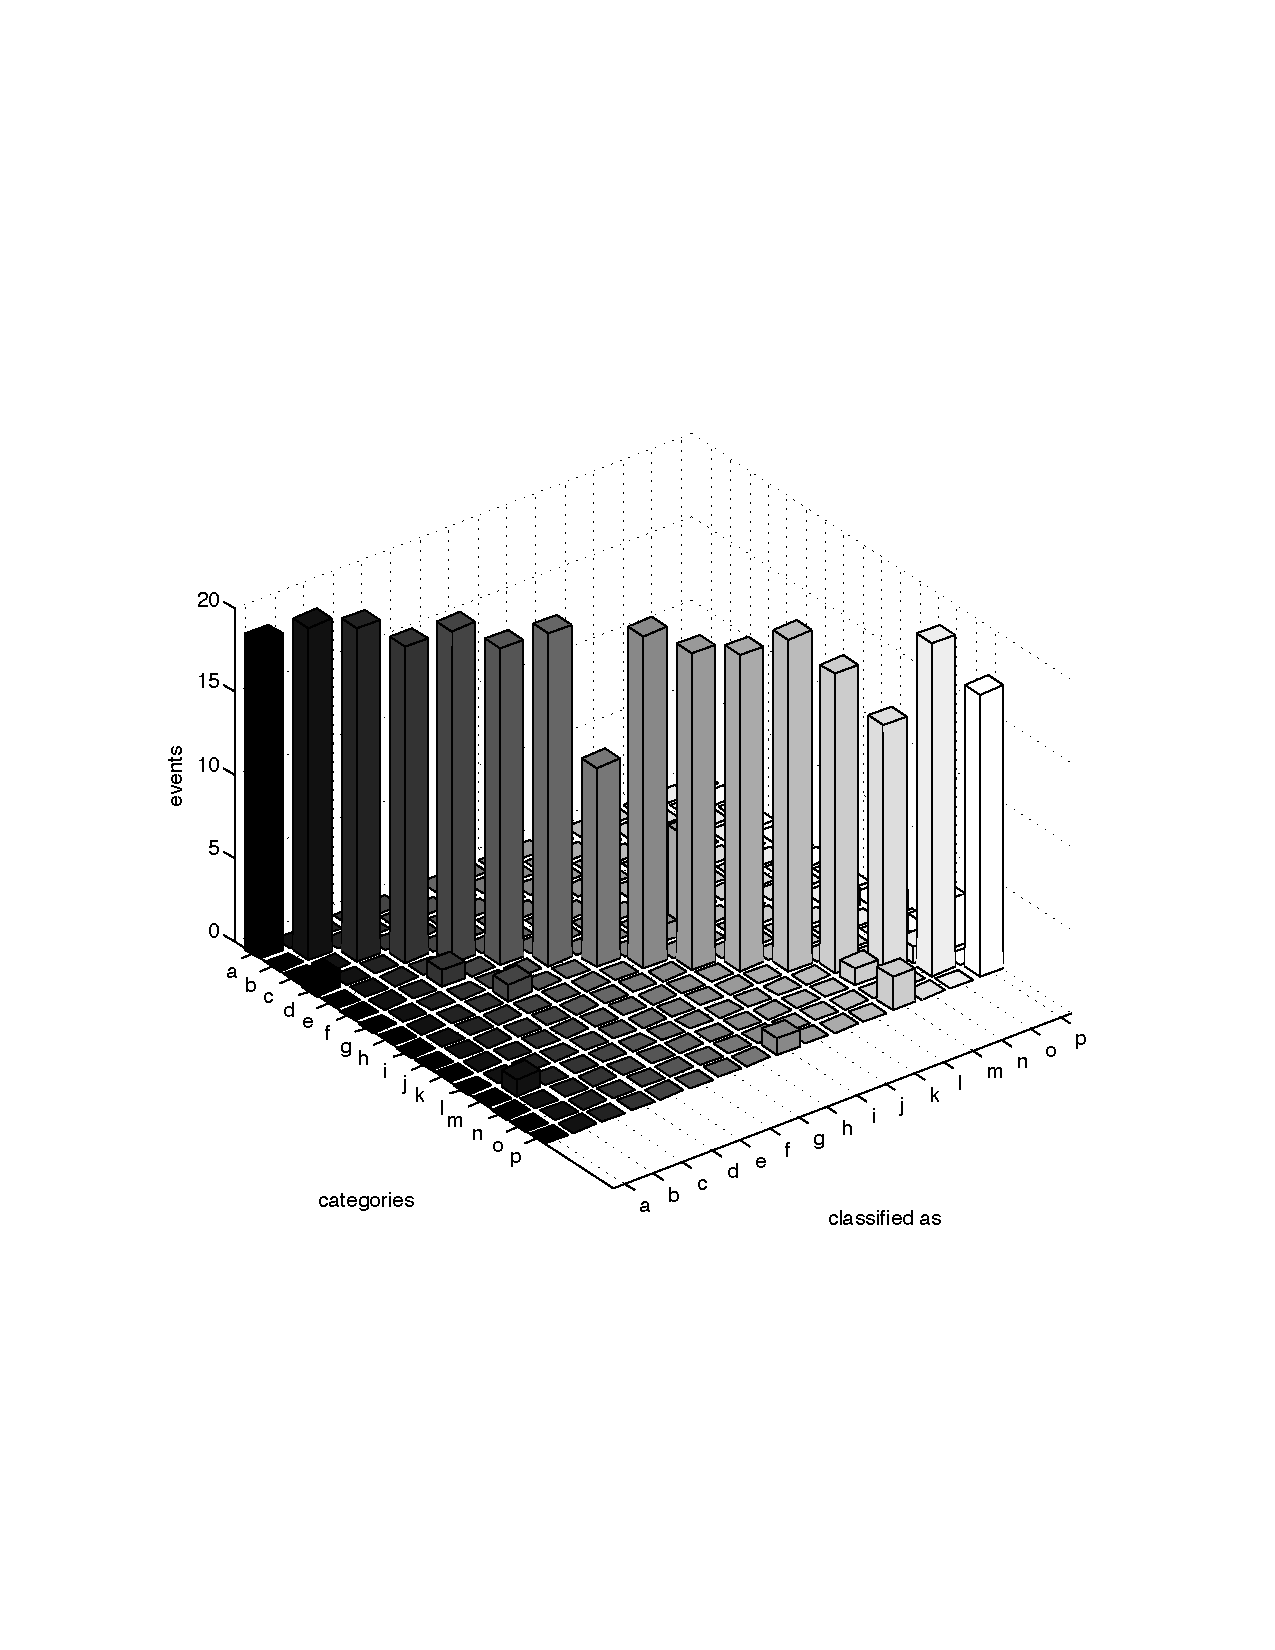
\includegraphics[trim=10 0 10 0,clip,height=1.9in]{93perOffice.pdf}
  	\label{fig:conf1}}
  \subfloat[]{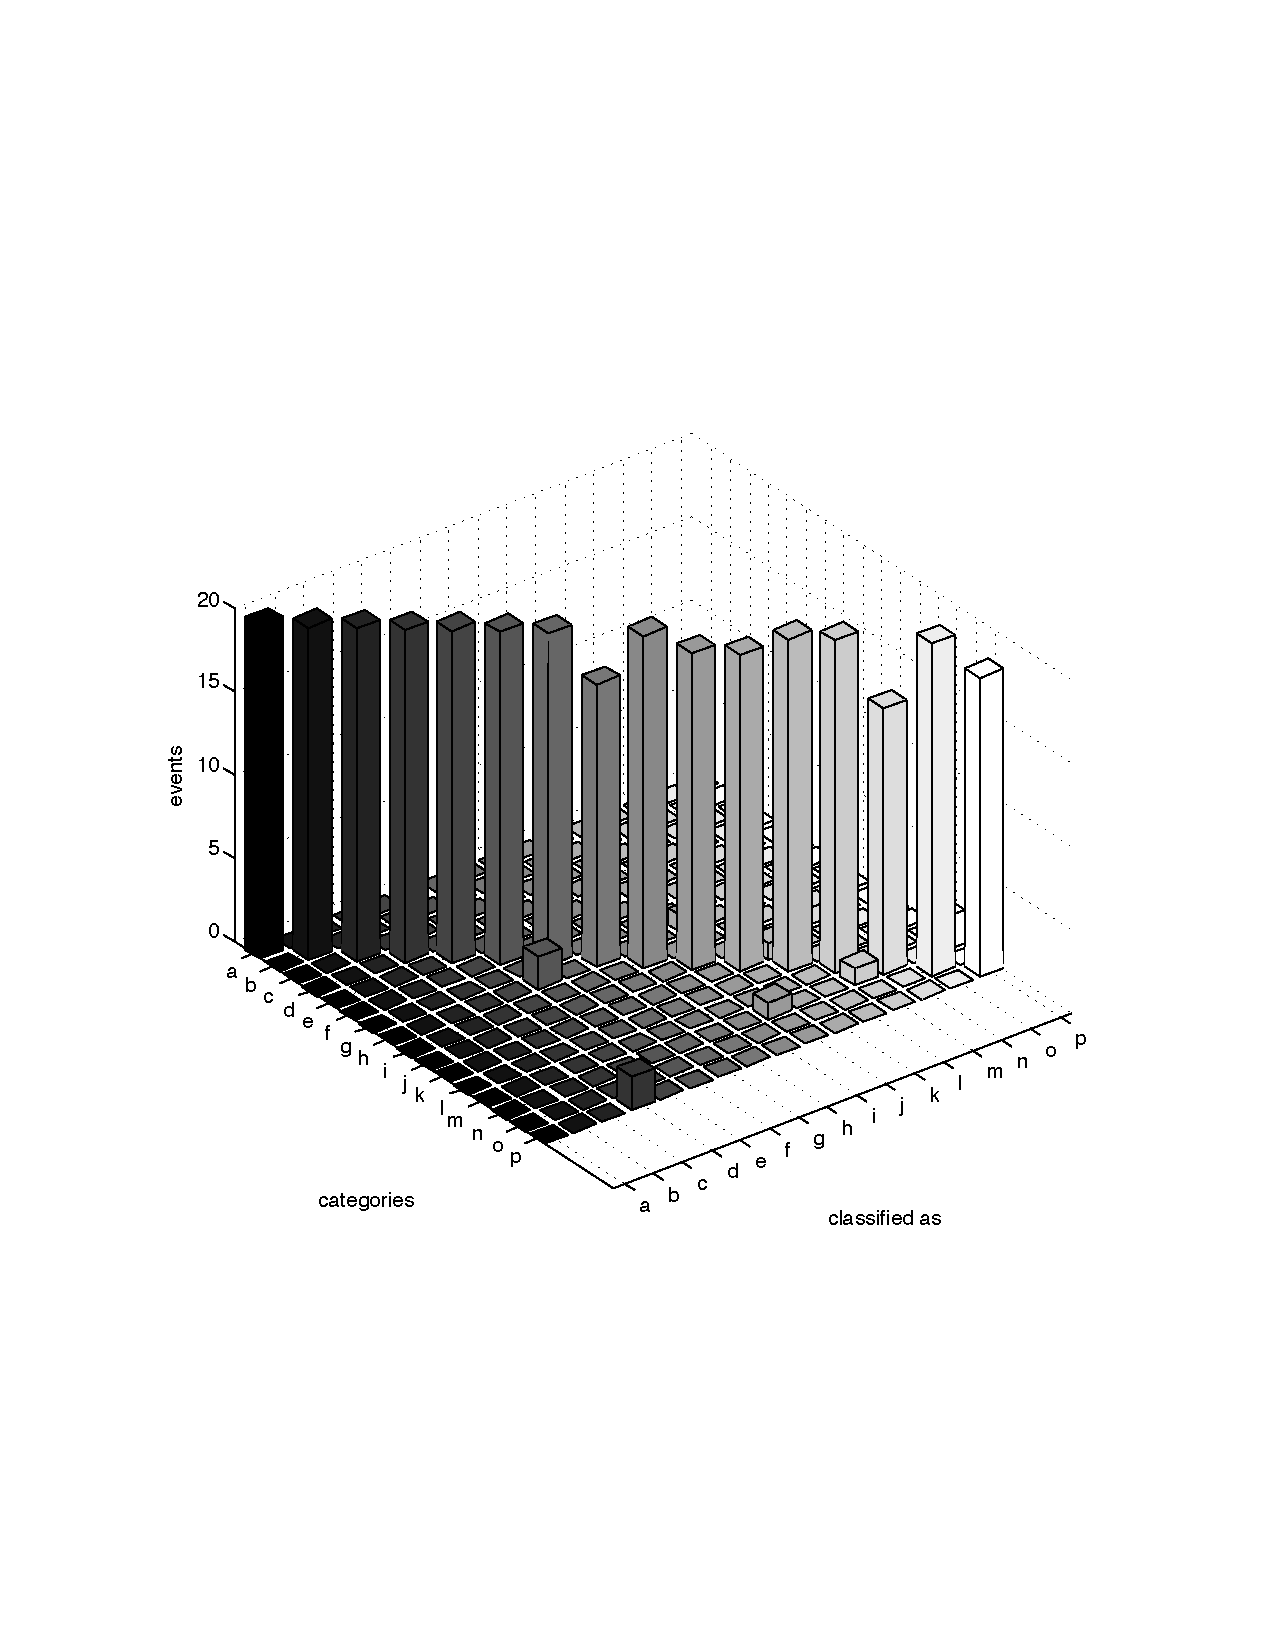
\includegraphics[height=1.35in,height=1.9in]{96perOffice.pdf}
  	\label{fig:office2nd}}
	\\
  \subfloat[]{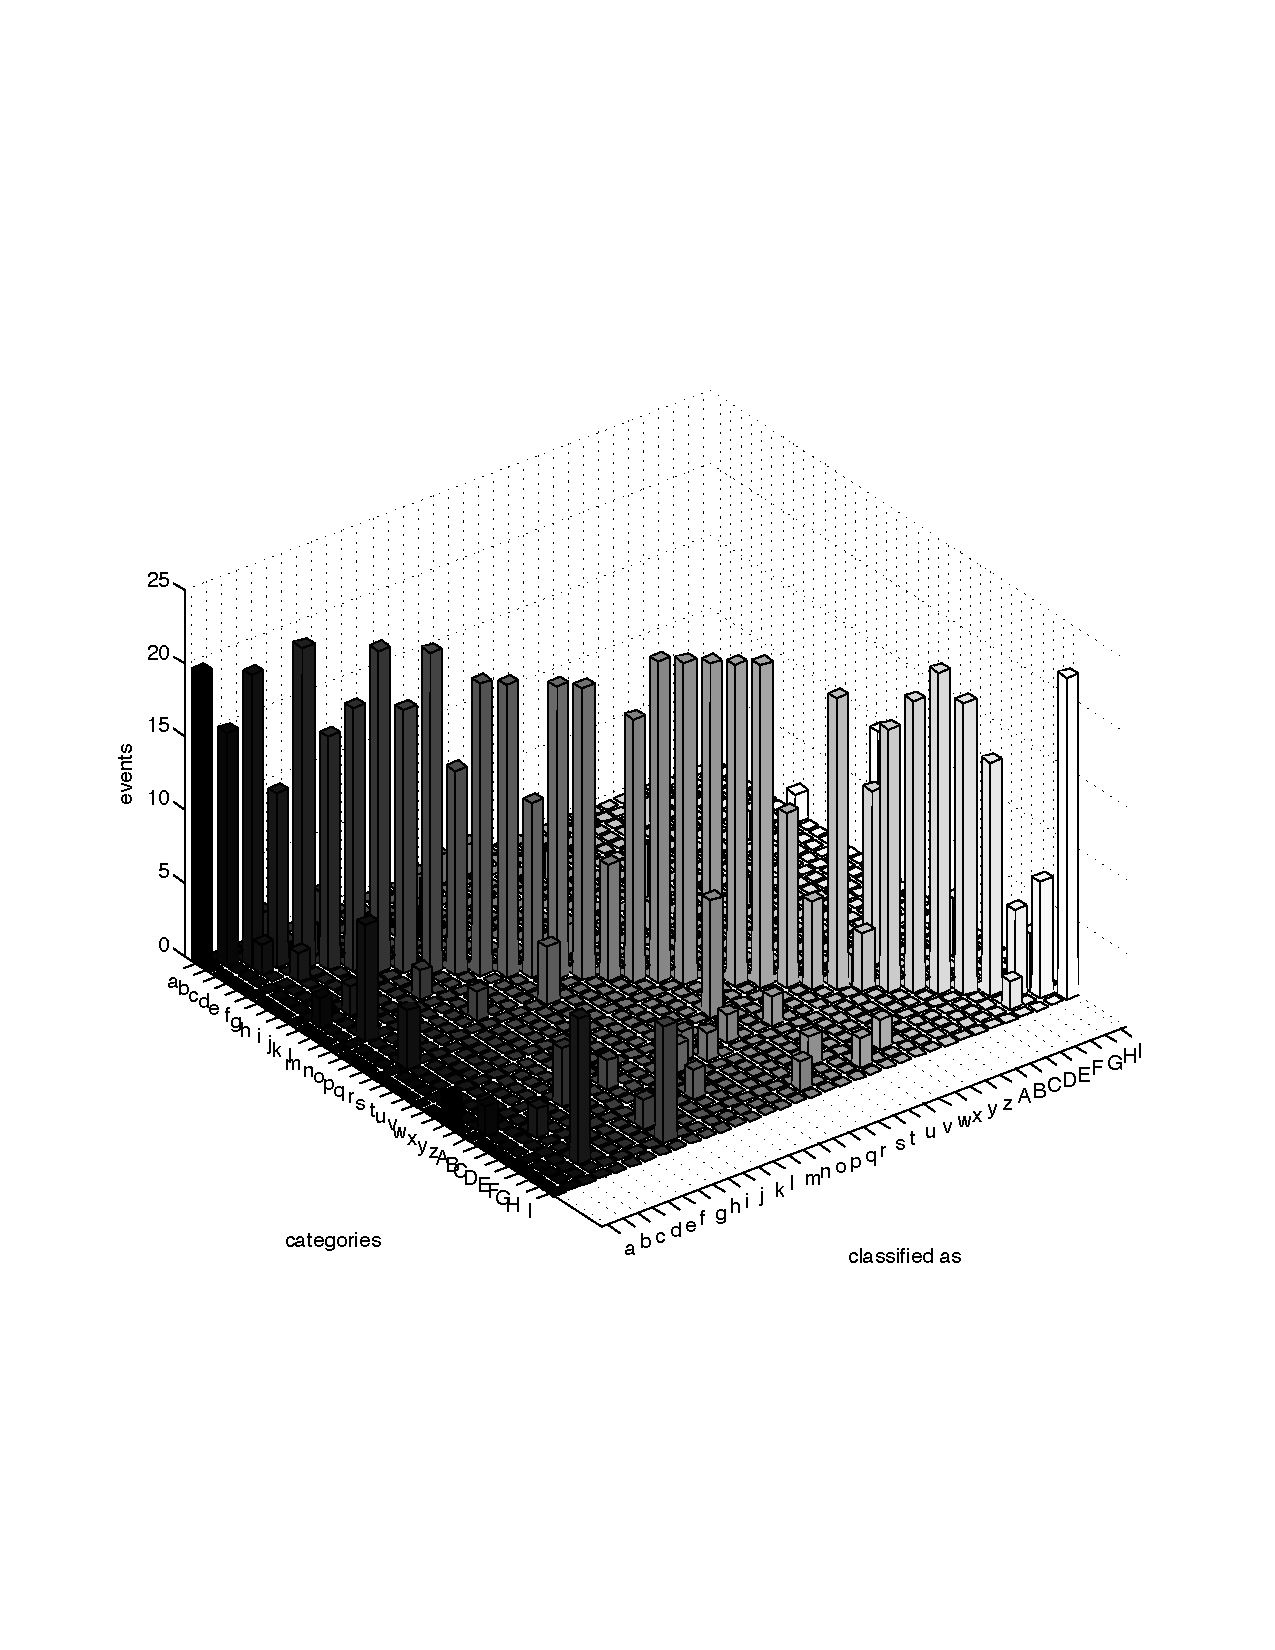
\includegraphics[trim=10 0 10 0,clip,height=1.9in]{80perAll.pdf}
  	\label{fig:all}}
  \subfloat[]{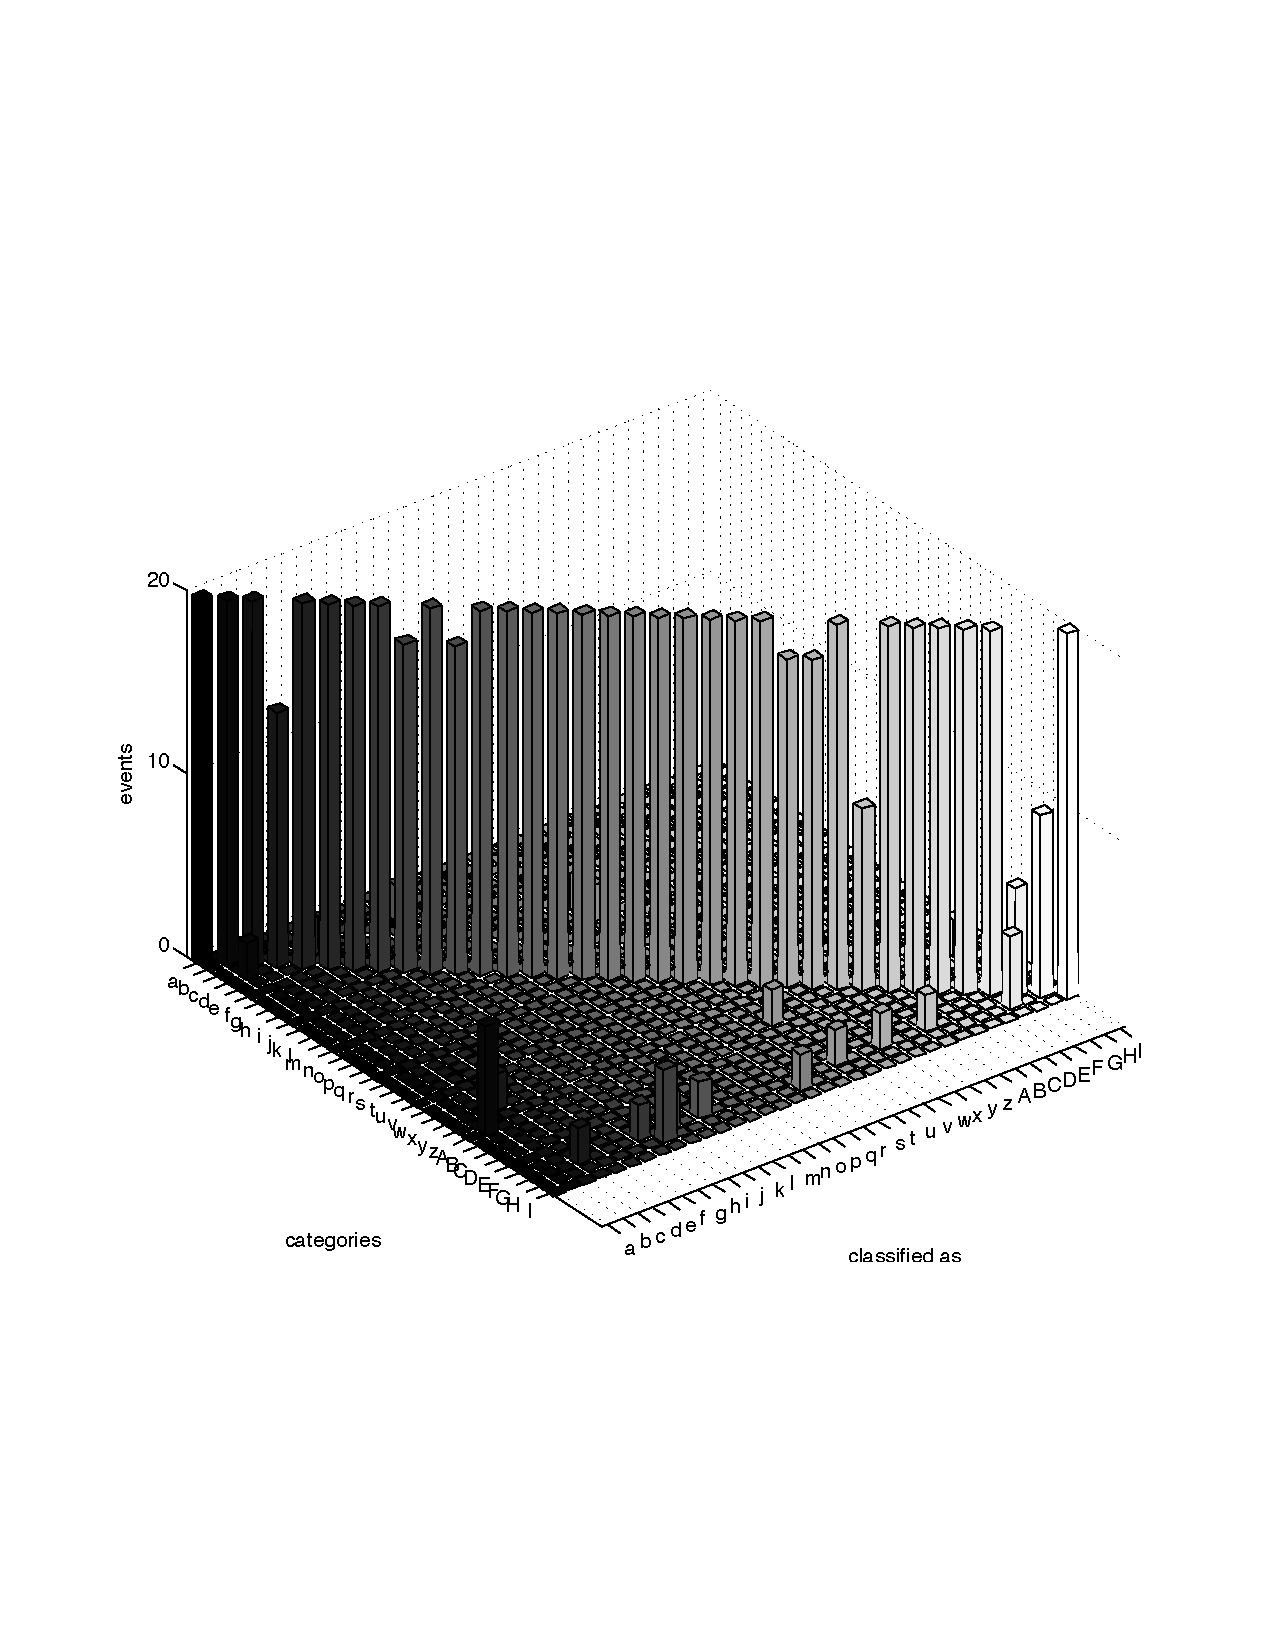
\includegraphics[height=1.35in,height=1.9in]{94perAll.pdf}
  	\label{fig:all3rd}}
  \end{center}
\caption[Confusion matrices for the distinct classes]{ The confusion matrix~\subref{fig:conf1} of the office
 using the lookup-table fusion compared with the confusion matrix
 in~\subref{fig:office2nd} using the second best locations in
 addition to the lookup-table. The same is depicted, below only for
 all the 35 different semantic locations. Figure~\subref{fig:all}
 shows the classification of the lookup-table fusion, whereas
 Figure~\subref{fig:all3rd} shows the lookup-table fusion considering
 up to the 3rd best.}
\label{fig:confma}

\end{figure}

\paragraph{Living room}
In the living room scenario, most of the samples from 7 of the 9
locations can be classified correctly. A lot of the sofa instances are
confused with the chair, as the chair is also padded. This is the
worst confusion occurring. Again the classifiers perform poorly for
window ledge category. The living room classification accuracy starts
with 60\% for acceleration alone, and goes up to 87\% for the
vibration sound. In this scenario, the sound sampling is worse than
the vibration methods at 85\%. This explains also why the fusion
methods on top of the vibration work so well and are nearly as good as
the fusion over all methods, at 88 and 89\% respectively. The fusion
over all methods is just 0.5\% better, namely 89.5\%. Only a very
small number of events (one to two) are corrected by this fusion. In
the "2nd best evaluation" the accuracy ranges from 66\% for
acceleration alone, up to 97\% for the lookup-table fusion over all
methods. Here also, the acceleration and sound vibration fusion do
extremely well with 93\% and 96\%.

\paragraph{Apartment}
In the apartment case, the worst miss-classification happens in the
cupboard class, which is confused with the desk. Both are made out
of the same wood. The radiator class is also confused with several
other classes. Here the acceleration accuracy is at 65\%, the
vibration sound at 81\%, sound sampling at 90\%. The fusion using just
the vibration method is at 82\% and 84\% respectively. As with all the
fusion examples the lookup-table performs slightly better. Finally, the
fusion techniques on all 3 modalities are all over 90\%. Taking a
look at the "2nd best evaluation", there the accuracy ranges from 80
\% for acceleration to up to 99\% for the look-up table over all three
classifiers.

\paragraph{Combined over all rooms (35 classes)}
As expected, more classes signify a worse classification rate. The ledge classes perform
poorly, even in the 2nd and 3rd best evaluation. Also, one of the
table classes does badly and is confused with several other classes.
The classification accuracy over all 35 semantic locations is
expectably lower than those of the single scenarios, ranging from 26\%
for acceleration, 51\% for vibration sound, 74\% for sound sampling,
over 52\% for the vibration fusion, up to 78\% for the fusion of all
methods. The 2nd and 3rd best evaluations look considerably
better. Second best is up to 90\%. Third best reaches 94\%. 

\paragraph{Abstract Location Classes}
For the abstract classes, the iron and wood classes are easily
confused, as are the stone and glass. Acceleration classification
alone performs reasonably well, at 63\% compared to the other
scenarios. Sound vibration is better at 69\%. As nearly always, sound
sampling performs better than the vibration method, at 81\% accuracy.
Regarding the fusion techniques, there is also nothing surprising. The
vibration fusion majority decision is at 70\%, the vibration
lookup-table around 71\% accuracy. The two fusions based on all
methods are at 83\% for the simple majority decision case and 86\% for
the lookup-table. Allowing the second best classification method, one
can stem up the performance to 92\% for the lookup-table fusion
method.

\begin{figure}[t]
  \begin{center}
  \subfloat[]{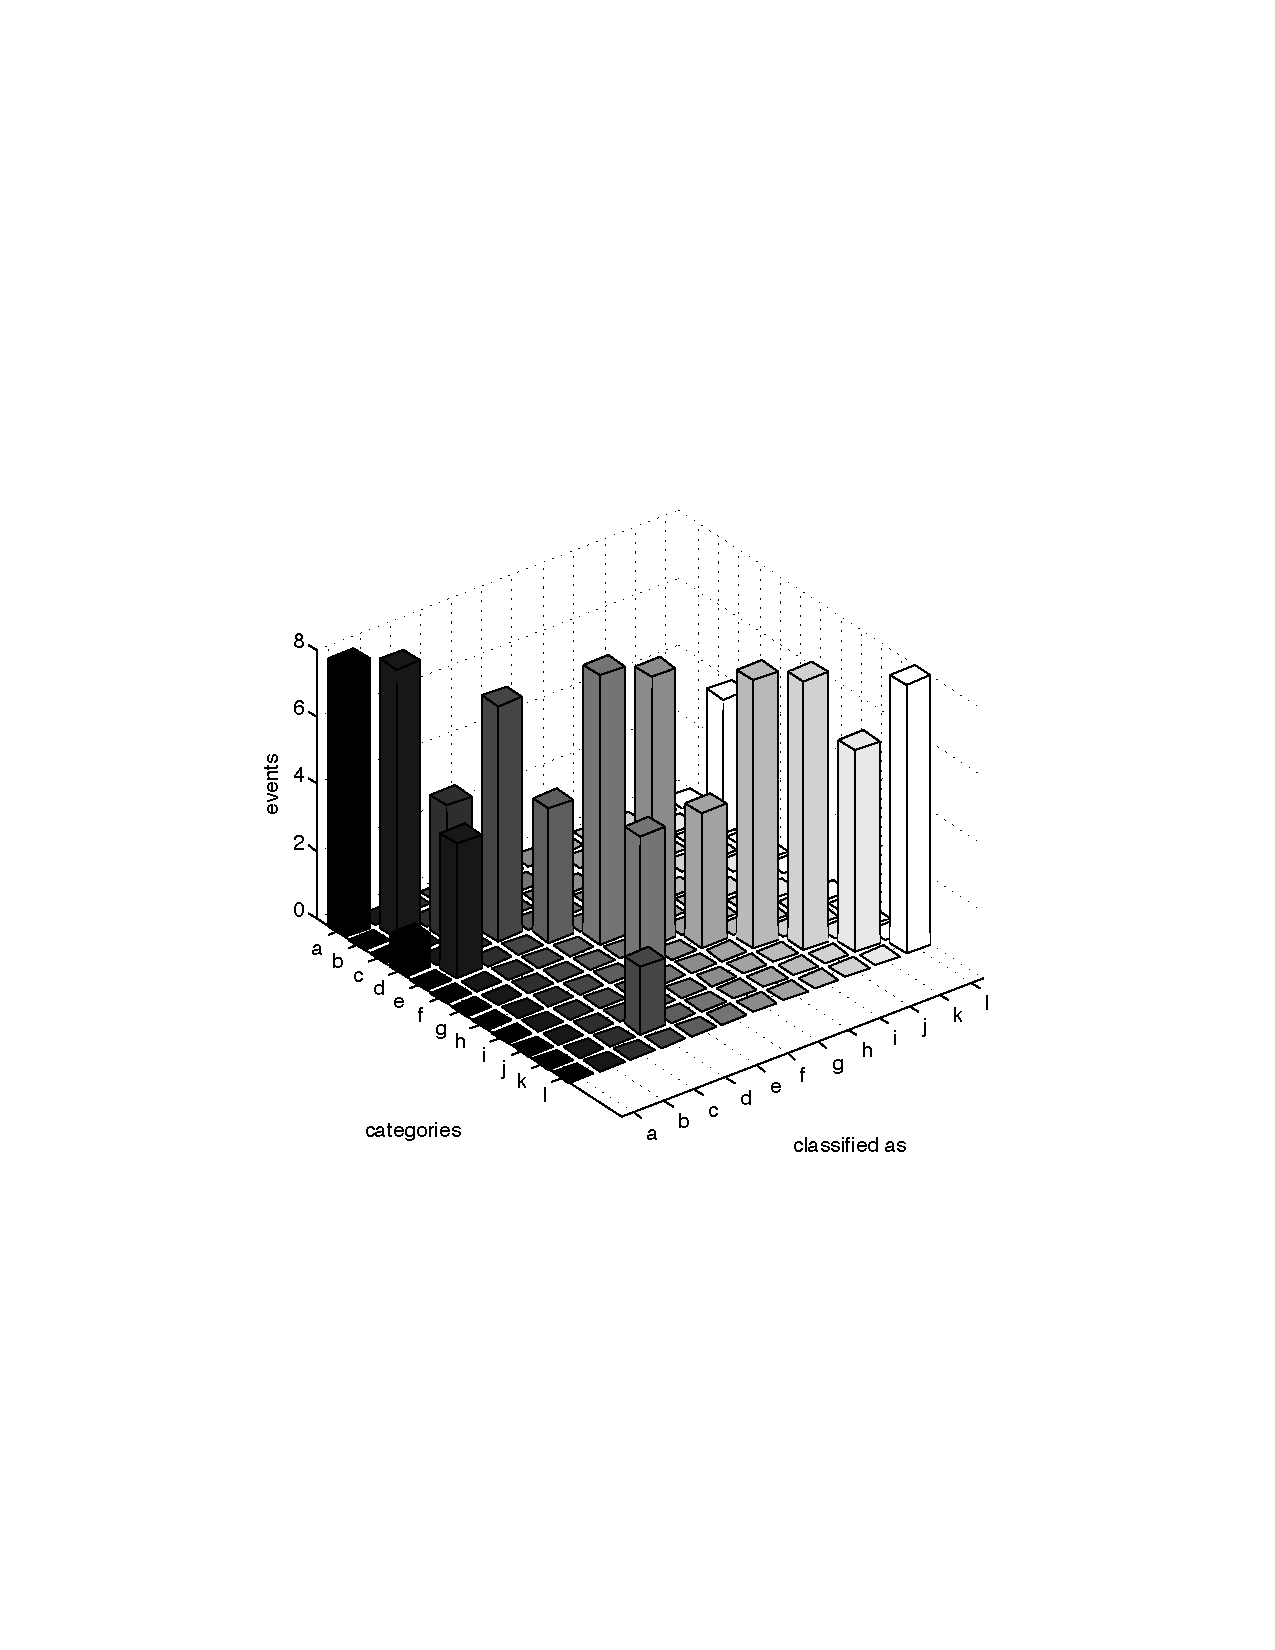
\includegraphics[trim=10 0 10 0,clip,height=2.0in]{surf.pdf}
  	\label{fig:surf}}
  \subfloat[]{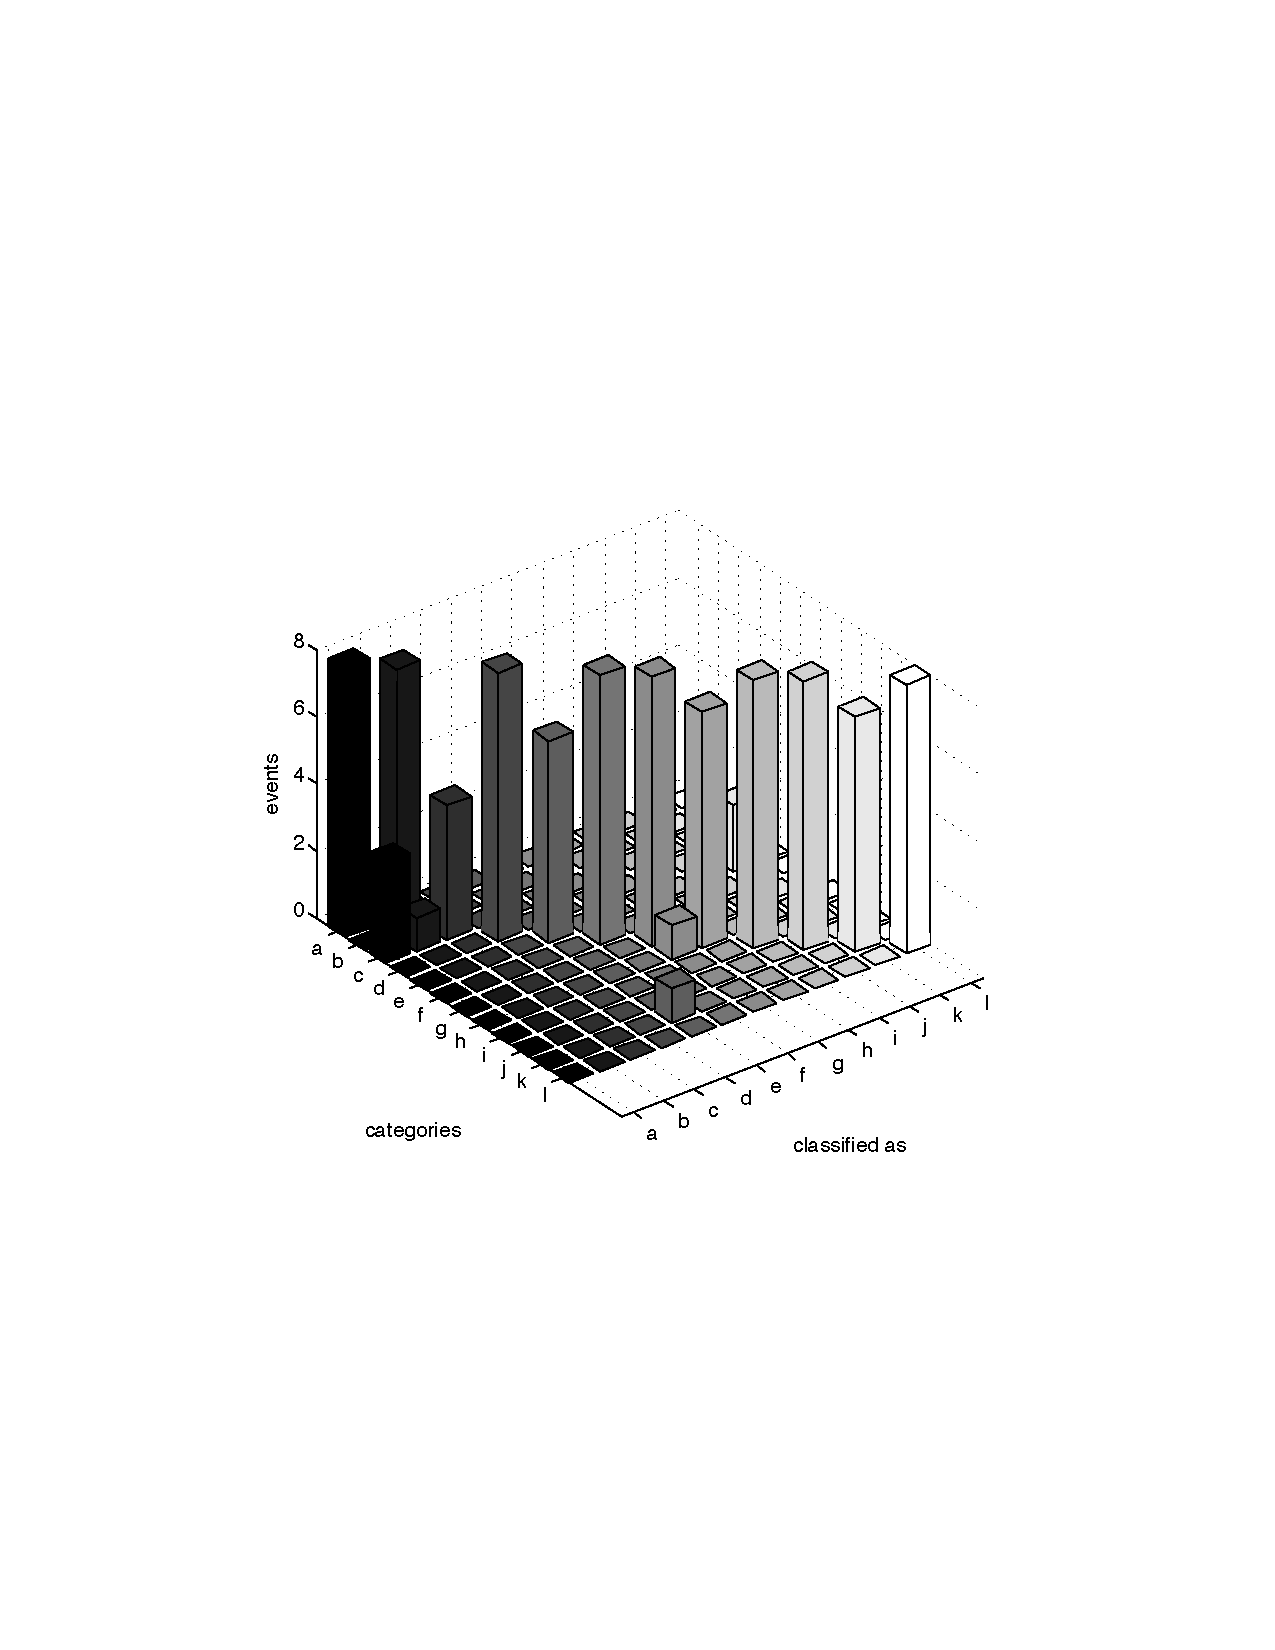
\includegraphics[height=1.35in,height=2.0in]{surf2nd.pdf}
  	\label{fig:surf2nd}}
  \end{center}
\caption[Confusion matrices for the abstract classes]{ Confusion matrix~\subref{fig:surf} of the abstract classes
 compared with the corresponding 2nd best confusion matrix
 in~\subref{fig:surf2nd}} \label{fig:confmasurf} \end{figure}



\subsection{Lessons Learned and Implications} 


\paragraph{Overall Performance}
The performance of the system is extremely inhomogeneous with respect
to the classes. There is a large proportion of classes for which the
classification is perfect or near perfect, and a small one with very
poor performance (see confusion matrices in figures \ref{fig:conf1},
\ref{fig:office2nd}, \ref{fig:all} and \ref{fig:all3rd}. As a
consequence the overall recognition accuracy figures are strongly
influenced by a few classes. This
is best exemplified by the abstract location type confusion matrix and
3rd best evaluation of the combined specific location classes. As can
be seen in the plots \ref{fig:conf1}, \ref{fig:office2nd},
\ref{fig:all} and \ref{fig:all3rd} the former has 8 perfect or near
perfect classes, 1 reasonably good class and 3 very poor ones. The
latter has 31 perfect to very good (27 perfect) classes, 1 mediocre
one and 3 very poor classes.
 

\paragraph{Class by Class Performance}
For some of the classes such as the inside and outside pocket, poor
performance is expected, as they are included to test the limits of
the system. In fact the recognition for these locations is better than
expected. Better than expected recognition has also been achieved in a
number of locations that were included as 'hard cases' such as the
backpack and the trousers pocket. Surprising is the poor performance
of the window ledge and the radiator. At this stage we have no
verified explanation. One possibility is a spatial inhomogeneity of
those symbolic locations. On the ledge, sound sampling is certainly
different depending on whether the speaker faces the window or faces
away from it. 
 
\paragraph{Value of the 2nd and 3rd Best Evaluation}
The performance of the system is particularly appealing for
applications that can accept a choice of two or three most probable
locations as system output. This has already been mentioned for the
case of 3rd best evaluation of the 35 combined symbolic locations. For
the other data sets even allowing just the 2nd best pick produces
close to perfect recognition for the vast majority of classes.

\paragraph{Value of Different Classification Modalities}
While it is to be expected from the discussion in \ref{sec:approach}
that sound sampling produces the best results and acceleration
the poorest, the difference between the two is larger than we
expected. In particular, the fact that in most cases little is gained
by adding acceleration and vibration sound to the sound fingerprint is
surprising. On the other hand, combining vibration sound and
acceleration often produces significant gains.


\paragraph{Significance of Training Set Size}
For the specific location mode the user needs to train the system for
every single relevant location. Thus the training effort is a
significant issue. As shown on the example of the office scenario in
figure \ref{fig:speaker} the system starts to display significant
recognition performance at around 5 training examples and stagnates at
about 10. We have found this behavior to be typical for all the
specific location mode scenarios. 


%
%\subsection{Paper Contributions and Organization}
%From the above discussion it can be seen that
%symbolic localization of objects with no external infrastructure
%and simple sensors suitable for small, cheap nodes is an open
%problem. This paper proposes a solution for this problem. 
%In terms of hardware the solution requires only a microphone, an
%accelerometer, a small speaker capable of emitting 'beeps' and a
%miniature vibration motor. 
%An important feature of our method is the fact that it can be used on
%both specific locations (e.g. my 'kitchen table'), and abstract location
% types. 
%
%We discuss the physical principle, key issues,
% and limitations
% behind our approach (section \ref{sec:approach}). 
%We then provide a detailed description of the recognition algorithm,
% including, feature computation,classification, and classifier fusion
% (section \ref{sec:recognition}). Finally, 
%we validate our method on an extensive, realistic data set (section
%\ref{sec:experimental}). The data set contains a total of over
%1200 measurements from 35 specific locations (taken from 3 different rooms)
%and 12 abstract location classes. The location were chosen to include
%examples that demonstrate the limits of the method such as an attempt
%to distinguish between the inner and the out pocket of the same jacket
%and between table and a book shelve both made of identical material.
%The data points at each symbolic location area taken at a number of randomized
%spots to ensure representativity.
%
%Despite such challenging evaluation our method produces promising
%results. On room bases (16, 9 and 10 locations) we
%arrive at an accuracy of between 89 \% and 93 \% with the correct answer
%being in the to 2 first picks of the classifier between 97 \% and 99 \% of the
%time. 
%With all 35 locations from the 3 rooms in one data set 
%the recognition goes down to 81 \%. However we still get the correct
%answer in the top 2 picks of the classifier 91 \% and in the top 3 94 \% times. 
%
%
%\section{Approach Overview}
%\label{sec:approach}
%\subsection{The Method}
%
%\paragraph{General Principles Behind the Recognition}
%In abstract terms the above method is about analyzing the response
%of the environment to a mechanical 'excitation' with different frequencies. 
%By vibrating the device we
%provide a low frequency (a few Hz) relatively high intensity (as
%compared to sound) source of excitation. By emitting fixed frequency
%'beeps' we generate different, low intensity high frequency stimuli.  
%The accelerometer detects the low frequency response (in our case up
%to 15Hz due to sampling frequency of the used device limited at 30Hz),
%the microphone the high frequency part. 
%
%The response to the above stimuli falls into several categories. 
%First we get a low frequency response that
%directly mechanically couples to the vibrating object and is detected
%by the accelerometer. This response can range from a more or less
%complete absorption of the vibration energy (e.g. when the object is
%lying on pillow) to a resonant response where the 
%surface, on which or device is lying, joins in the vibration.
%This fact contains information on two things. For one, it can reveal if, and how
%the device is fixed (in the hand, in a tight pocket, lying freely). In
%addition it reveals how hard and elastic is the surface on which the
%device is placed. This information can be expected to reliably distinguish
%between soft surfaces such as a sofa and hard ones like a
%table. Distinction between several similarly hard surfaces (e.g. metal
%and stone) is difficult.
%
%Second, we get a high frequency response to the vibration, 
%which is essentially a sound from the device hitting the
%surface. Assuming that placement of the device does lead to this kind
%of response (it will not, if the device is in a soft pocket or say hanging),
%it is quite location specific. The sound depends not only on the
%surface material but also on the overall structure. 
%Thus a small, solid cube will produce a different sound
%then a large thin surface, even if both are made of the same
%material. Finally, objects light and close enough to the device to
%be influenced by the vibration (e.g. a key chain) might also
%contribute to the sound. In general, this is a source of noise rather
%then usable information. Figures~\ref{fig:soundVib} show two different vibration spectra.
%
%
% Third, we get a high frequency response from the beeps which
%is given by the absorption spectrum of the environment. 
%\footnote{Note that the absorption also influences
%the sound caused by the device vibration.}
%Clearly this response is only useful if it comes from the immediate
%vicinity of the device. This can either be the surfaces on which the
%device is lying or, if the semantic location is a closed compartment, the
%walls of this compartment (see next section for a discussion of
%microphone placement issues). 
%It is well known that the acoustic absorption spectrum is a distinct
%material property. The topic has been extensively studied in the
%context of musical instruments and sound isolation in
%construction (\cite{olson1967mpa}). Typically the absorption is given at discrete
%frequencies as a fraction of the perfect absorption at an open window
%(lack of any reflecting surface) of equal area.
%As an example we consider the following coefficients from \cite{olson1967mpa}
%\\
%\noindent
%\begin{tabular}{|l|c|c|c|c|c|c|}
%\hline
%frequency & 128 Hz &	256 Hz &	512 Hz &	1,024 Hz &
%2,048 Hz & 	4,096 Hz \\
%\hline 
%concrete unpainted & 0.010&	0.012&	0.016&	0.019&	0.023&	0.035 \\
%brick wall painted & 0.012&	0.013&	0.017&	0.020&	0.023&	0.025 \\
%carpet on concrete (0.4inch) & 0.09 &	0.08 &	0.21 &	0.26 &	0.27 &
%0.37 \\
%\hline 
%\end{tabular}
% 
%The above clearly demonstrates that, in principle, even seemingly similar materials
%can be separated with a small number of discrete frequencies. 
%

\section{Excursion: Sensor Dependencies}

The successful application of our method is
highly dependent on the microphone/ speaker placement and the type of
vibration motor. A quick experimental setup illustrates this
dependence.


\begin{figure}[t]
\centering  
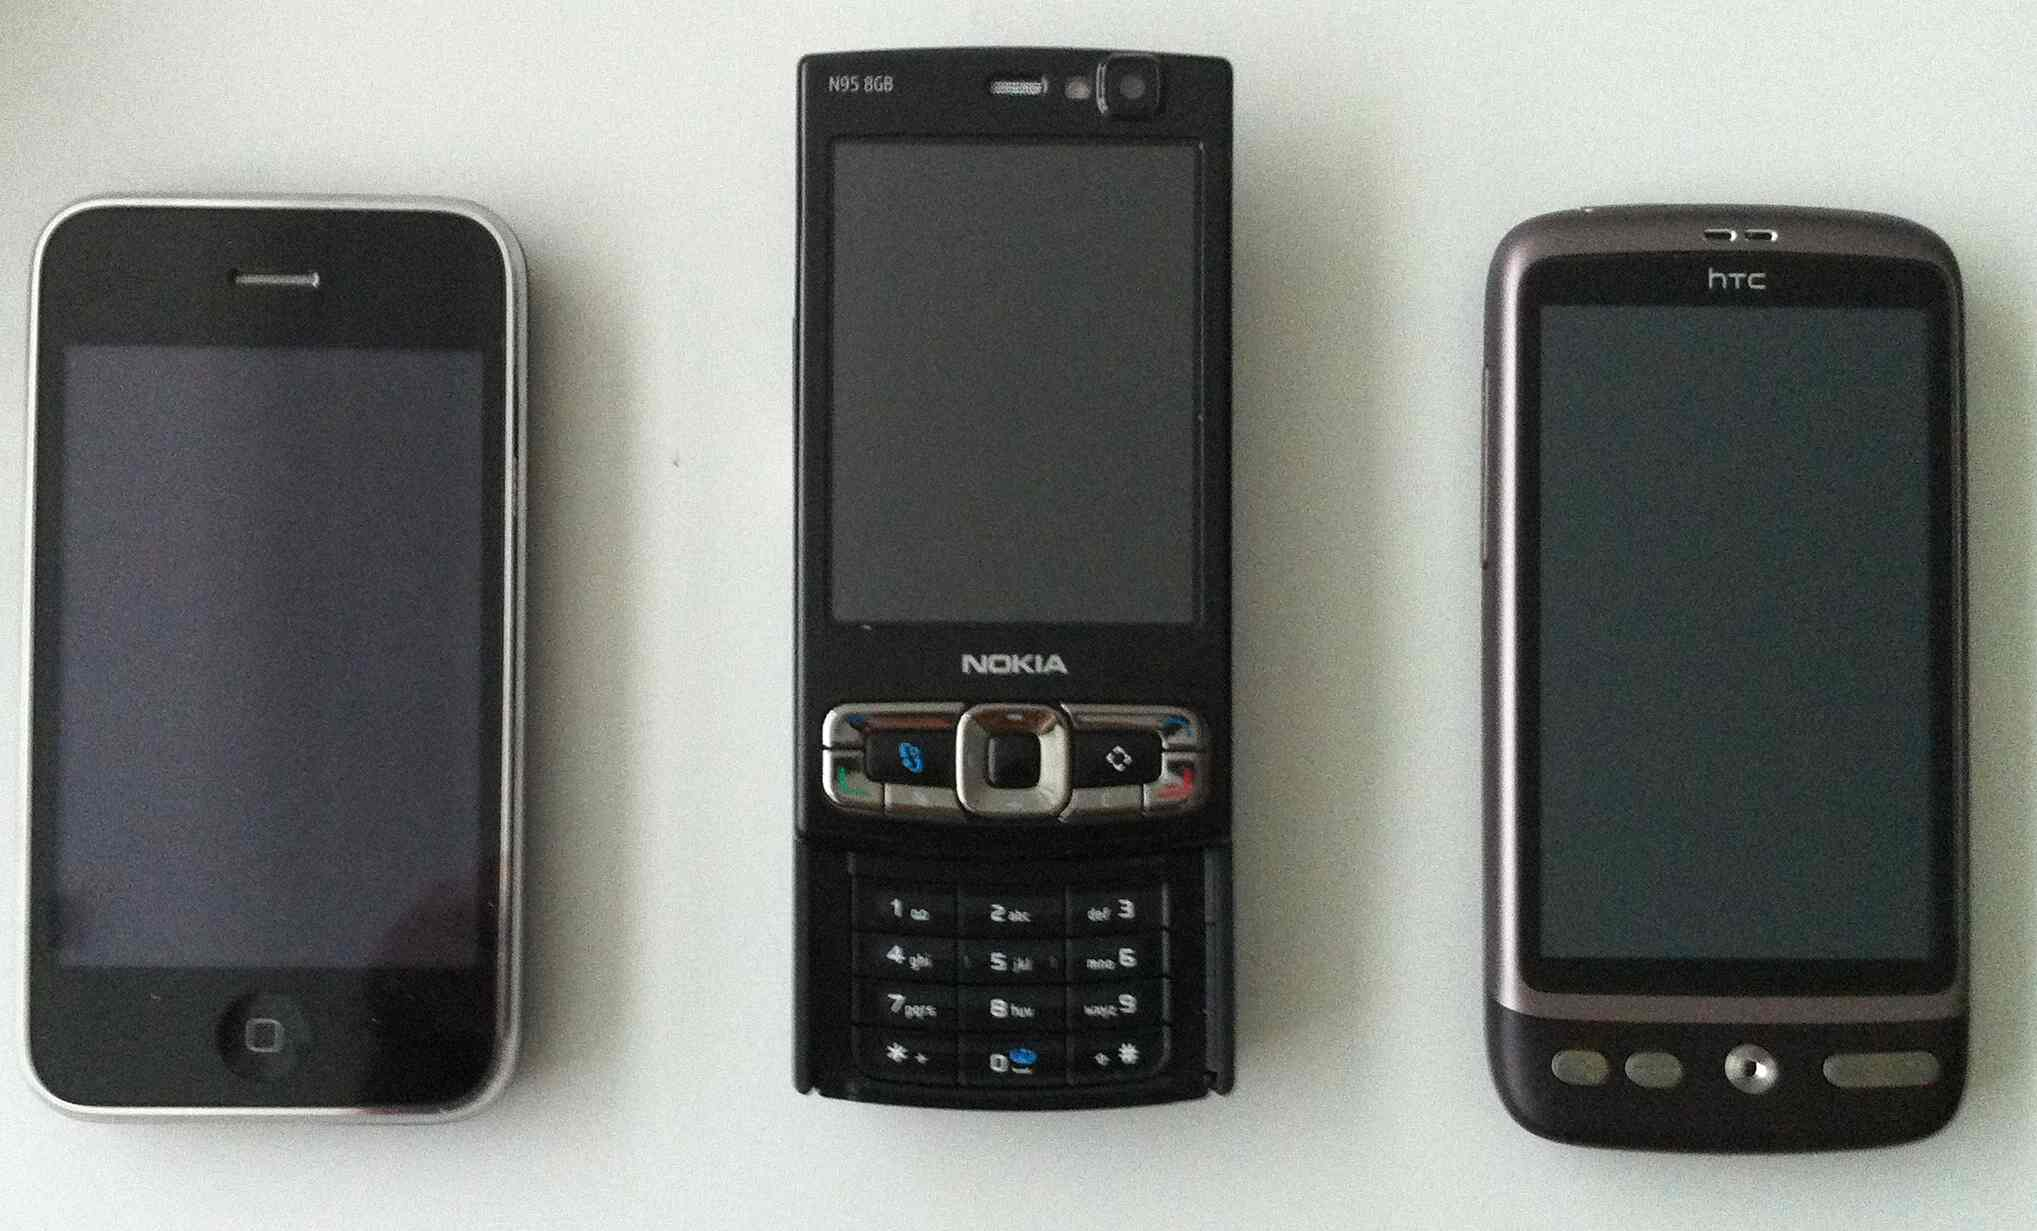
\includegraphics[scale=0.15]{mobiles.jpg}
\caption[Smartphones]{The three different mobile phones used for sensor
 comparisons: the iphone 3gs, nokia n95 and the htc
 desire.} \label{fig:mobiles}

\end{figure}

We use 3 regular smartphones, depicted in Figure~\ref{fig:mobiles} and
pick 4 locations from the living room scenario: desk, floor, sofa and
stereo. Each mobile performs the experimental procedure outlined in
the section above 5 times.


\begin{table}[ht]
\caption[Smartphone classification comparison]{Classification comparison for 4 locations from the living
 room scenario using frame-by-frame classification.}
\label{table:depend}
\begin{tabularx}{\textwidth+10pt }{lcccccc}
\toprule
mobile & htc desire &n95 &iphone 3gs& N 5500 Sport\\
\midrule
fingerprint & 45 \% & 60 \% & 47 \% & 100 \%\\
fingerprint (upside down) & 92 \% & 87 \% & 90 \% & 100 \% \\
vibration & 45 \% & 79 \% & 23 \% & 84 \% \\
vibration (upside down) & 43 \% & 83 \% & 25 \% & 87 \% \\
\bottomrule
\end{tabularx}
\end{table}

The classification results in Table~\ref{table:depend} show a high
dependency between the speaker /microphone placement and the
accuracy. Each phone shows respectable results with microphone and
speaker placed towards the surface using the sound fingerprint.
However, if the phones are placed with the microphone on the top (as a
phone is regularly put on a desk), the rates vary strongly, with the
N5500 being by far the best, as it has a separate speaker still facing
the surface.

Another important lesson to learn: the vibration classification seems
not that affected from the rotation of the devices. Yet, the vibration
motor and intensity seem crucial here. The HTC and iphone are
equipped with motors operating at a far lower intensity compared to
the ones built into the Nokia models. This is also the reason for the
lower classification performance.


\section{Discussion}
 
Summarizing the issues from section~\ref{sec:issues} and the
experimental results from section~\ref{sec:results} we conclude the
following:

\begin{enumerate}
\item The proposed method is well suited for low end, simple sensor
 nodes and smart objects and requires no additional positioning infrastructure. 
\item The key source of information is sound sampling. Thus if
size is critical the vibration motor can be dropped.
\item The system can reliably (90\% and more accuracy) resolve a 
sufficient number of specific locations to cover one room or a small flat. It is advisable to combine our system with room level positioning.
\item The performance of the system is extremely inhomogeneous with respect to
the classes, with most classes being recognized with high accuracy and a
few "rogue" classes showing very poor performance.
\item Settling for the two or three best picks instead of a crisp single
 classification greatly increases the number of locations that are
 reliably recognized and the tolerance towards the "rogue" classes. 
\item If training by the user is an issue, the abstract location class
 mode offers a possibility to provide "pre-trained" systems at the
 cost of more "fuzzy" location information. \end{enumerate}

Key points to investigate in the future are improved vibration
sampling (using different amplitudes and frequencies to improve
acceleration based performance), an investigation of the sources of
errors on the problematic classes, more elaborate fusion methods, and
a combination with radio signal strength based location methods. 

Summarizing, this chapter treats detecting wether a device is carried on
the body or placed in the environment as a special case of recognizing
its symbolic placement. The active sampling method presented gives a
specific solution to this recognition problem with merits and
limitations discussed above. Moving away from the detecting
environmental placements the focus is now on on-body sensing for the
remainder of this thesis, centering on how to perform activity
recognition independent of device placement and orientation,
compensating for displacements. Thus after dealing with symbolic
object placement containing locations on and off body, we focus on
determine the on-body placement of a device.


%\cleardoublepage
%\addcontentsline{toc}{section}{Bibliography}
\bibliographystyle{abbrv}
\bibliography{onoff}

